%% The '3p' and 'times' class options of elsarticle are used for Elsevier CRC
%% Add the 'procedia' option to approximate to the Word template
%\documentclass[3p,times,procedia]{elsarticle}
\documentclass[3p,times]{elsarticle}

%% The `ecrc' package must be called to make the CRC functionality available
\usepackage{ecrc}

%% The ecrc package defines commands needed for running heads and logos.
%% For running heads, you can set the journal name, the volume, the starting page and the authors

%% set the volume if you know. Otherwise `00'
\volume{00}

%% set the starting page if not 1
\firstpage{1}

%% Give the name of the journal
\journalname{Journal of Parallel and Distributed Computing}

%% Give the author list to appear in the running head
%% Example \runauth{C.V. Radhakrishnan et al.}
\runauth{P. Li et al.}

%% The choice of journal logo is determined by the \jid and \jnltitlelogo commands.
%% A user-supplied logo with the name <\jid>logo.pdf will be inserted if present.
%% e.g. if \jid{yspmi} the system will look for a file yspmilogo.pdf
%% Otherwise the content of \jnltitlelogo will be set between horizontal lines as a default logo

%% Give the abbreviation of the Journal.  Contact the journal editorial office if in any doubt
\jid{procs}

%% Give a short journal name for the dummy logo (if needed)
\jnltitlelogo{J. Parallel Distrib. Comput.}

%% Provide the copyright line to appear in the abstract
%% Usage:
%   \CopyrightLine[<text-before-year>]{<year>}{<restt-of-the-copyright-text>}
%   \CopyrightLine[Crown copyright]{2011}{Published by Elsevier Ltd.}
%   \CopyrightLine{2011}{Elsevier Ltd. All rights reserved}
\CopyrightLine{2014}{Published by Elsevier Ltd.}

%% Hereafter the template follows `elsarticle'.
%% For more details see the existing template files elsarticle-template-harv.tex and elsarticle-template-num.tex.

%% Elsevier CRC generally uses a numbered reference style
%% For this, the conventions of elsarticle-template-num.tex should be followed (included below)
%% If using BibTeX, use the style file elsarticle-num.bst

%% End of ecrc-specific commands
%%%%%%%%%%%%%%%%%%%%%%%%%%%%%%%%%%%%%%%%%%%%%%%%%%%%%%%%%%%%%%%%%%%%%%%%%%

%% The amssymb package provides various useful mathematical symbols
\usepackage{amssymb}
%% The amsthm package provides extended theorem environments
%% \usepackage{amsthm}

%% The lineno packages adds line numbers. Start line numbering with
%% \begin{linenumbers}, end it with \end{linenumbers}. Or switch it on
%% for the whole article with \linenumbers after \end{frontmatter}.
%% \usepackage{lineno}

%% natbib.sty is loaded by default. However, natbib options can be
%% provided with \biboptions{...} command. Following options are
%% valid:

%%   round  -  round parentheses are used (default)
%%   square -  square brackets are used   [option]
%%   curly  -  curly braces are used      {option}
%%   angle  -  angle brackets are used    <option>
%%   semicolon  -  multiple citations separated by semi-colon
%%   colon  - same as semicolon, an earlier confusion
%%   comma  -  separated by comma
%%   numbers-  selects numerical citations
%%   super  -  numerical citations as superscripts
%%   sort   -  sorts multiple citations according to order in ref. list
%%   sort&compress   -  like sort, but also compresses numerical citations
%%   compress - compresses without sorting
%%
%% \biboptions{comma,round}

% \biboptions{}

% if you have landscape tables
\usepackage[figuresright]{rotating}

% put your own definitions here:
%   \newcommand{\cZ}{\cal{Z}}
%   \newtheorem{def}{Definition}[section]
%   ...


\usepackage{psfig}
\usepackage{graphicx}
\usepackage{textcomp}
\usepackage{amsmath}
\usepackage{amssymb}
\usepackage{longtable}
\usepackage{array}
\usepackage{algorithm}
\usepackage{algorithmic}
\usepackage{color}
\newcommand{\reminder}[1]{{{\textcolor{blue}{\bf (#1)}}}}
\newcommand{\tabincell}[2]{\begin{tabular}{@{}#1@{}}#2\end{tabular}}
\usepackage{url}



%-------------------------------------------------------------------------
% take the % away on next line to produce the final camera-ready version
%\pagestyle{empty}

%-------------------------------------------------------------------------
\begin{document}

\begin{frontmatter}

\title{Transformer: Run-time Reprogrammable Heterogeneous Architecture
  for Transparent Acceleration of Dynamic Workloads}


\author{Peilong Li}
\ead{Peilong\_Li@student.uml.edu}
\author{Yan Luo}
\address{University of Massachusetts Lowell, One University Ave, Lowell, MA, USA, 01854}
\author{Jun Yang}
\address{University of Pittsburgh, 4200 Fifth Avenue, Pittsburgh, PA, USA, 15260}

\begin{abstract}

Heterogeneous architectures face challenges on resource allocation to
cores and accelerators as well as transparent acceleration.  We
propose "{\em Transformer}", a run-time reprogrammable, heterogeneous
architecture with cores and reconfigurable logics for supporting
coarse-grained acceleration of dynamic, unpredictable workloads
presented in mobile and cloud computing environments. The architecture
allows run-time instantiation of one or more acceleration functions in
an on-chip reconfigurable logic in response to the demands of
compute-intensive software libraries. We design a hardware controller
and software wrapper functions to profile workloads, reprogram the
logic and invoke accelerators. Novel heuristics are derived to
schedule accelerator functions. We explore the optimal chip resource
allocation for cores and accelerators. Our simulation results show
that Transformer brings significant improvement on both performance
(up to 14x for single-type workloads and up to 2.3x for dynamic
workloads) and energy efficiency (up to 6.9x) for a wide range of
workloads.

\end{abstract}


\begin{keyword}
Accelerator \sep Transparent acceleration \sep Coarse-grain
\sep Heterogeneous architecture \sep FPGA
%% keywords here, in the form: keyword \sep keyword

%% PACS codes here, in the form: \PACS code \sep code

%% MSC codes here, in the form: \MSC code \sep code
%% or \MSC[2008] code \sep code (2000 is the default)

\end{keyword}

\end{frontmatter}


\section{Introduction}


Chip Multi-Processors (CMPs) have become the mainstream processors for
mobile, desktop, and cloud computing platforms due to their power
budget as well as their limits in terms of clock frequency scaling. While
thread-level parallelism can be well leveraged with CMPs
for throughput oriented applications \cite{CMP05}, the single-thread performance of
a processor still remains important to time critical workloads. Therefore,
various ASIC-based accelerators are utilized to improve single-thread performance. 

However, ASIC based on-chip accelerators do not respond well to
emerging dynamic workloads where applications come and go either on
demand or in an unpredictable manner. For example, the user of a smartphone may
install or uninstall apps at any time, leading to a changing mixture
of applications. A cloud computing platform such as Amazon EC2
\cite{amazon-ec2} can execute a variety of workloads submitted at arbitrary points in time from a user's Virtual Machine (VM) 
 including the Web \cite{Chen:2012jo}, data mining \cite{ec2-datamining}, as well as DNA sequencing
\cite{ec2-dna}.  The built-in static accelerators may not be needed for extended periods of time
or for certain workload mixes.  As a result, the static accelerators remain dormant during these time periods, 
culminating in the waste of silicon resources.

A complementary approach consists of using off-chip programmable hardware
accelerators such as GPUs and/or FPGAs to speed up complex workloads
\cite{GPUFPGA, fpga-acc}. However, due to the nature of conventional system architectures, 
such hardware acceleration units do not meet the stringent time requirements 
of delay-sensitive workloads. The aforementioned units are typically
connected to the processor cores through off-chip interconnects
(e.g., PCIe, QPI \cite{intel-qpi} or by way of HyperTransport
\cite{amd-hypertransport}), each of which has serious latency limits and therefore results in
significant delays with regards to the transfer of data. Thus, even with their extensive
parallel processing capabilities, FPGAs and GPUs are challenged to produce the anticipated levels
of increased speed.  
%Their performance advantages
%and flexibility in reprogramming cannot be harnessed to the full
%extent until an architectural change occurs on their interconnects to
%cores.

Leveraging on-chip accelerators in existing as well as new applications is a
non-trivial undertaking given the prohibitive redevelopment costs.  
%Allowing an applications' execution flow to be transparently directed to accelerators
%without any user intervention remains an interesting but unsolved
%issue. 
As new instructions are typically added to SoC
accelerators, rewriting and recompiling the application's code is
a requirement. Fine-grained accelerations also require compiler support \cite{Govindaraju:2012fn}. As the IPs for
FPGAs and programs developed for GPUs continually increase, it becomes more plausible
to incorporate them through coarse-grained acceleration. For example, an entire function, such as 3DES encryption,
can be sped up as an element of an existing software library, such as libopenssl. A library based
approach facilitates acceleration without incurring development or redevelopment costs. 

The power efficiency \cite{hamada09,thomas09} and performance benefits
of recently developed programmable hardware has been driving the momentum of
heterogeneous computing platforms that combine general-purpose cores
and reconfigurable logic for high performance computing (HPC) applications, 
for example the Convey HC-1 \cite{brewer09} and the Cray XD1 \cite{Ulmer:2005vh}.
However, the workloads in many computing environments
are far more dynamic than those in the HPC domain. The
fusion of general-purpose cores with programmable logic for
power-efficient computing has been inadequately researched in terms of
the architecture trade-offs between performance and power, transparent
acceleration, and accelerator-aware scheduling, all of which are
critical to the practical deployment of programmable heterogeneous
architectures.

The {\em Transformer}, a heterogeneous architecture solution consisting of 
general purpose cores along with on-chip programmable accelerator logic, is a
viable means to address the challenges introduced by the dynamic workloads that exist within a number of
emerging scenarios. The aforementioned solution differs from existing architectures in several ways.
First, the architecture consists of on-chip programmable
accelerators with general purpose cores.  By sharing the memory hierarchy
with the cores, the accelerators are promoted to first-class citizens and therefore
reduce latency by means of efficient access to the data stored within each of the cores.  
Second, sharing an accelerator unit among multiple acceleration functions
improves the utilization of the chip resources. Optimal area resource
allocation to the cores and the accelerators leads to improved performance as well as improved
energy efficiency. Given a set of resource constraints, the heuristics proposed maximize the memory
bandwidth utilization and lead to speedup improvements with respect to unpredictable workload
mixtures. Third, the architecture
enables transparent acceleration with novel middleware support,
significantly reducing deployment costs.  It is worth noting that,
while the programmable accelerator logic in the proposed architecture
could potentially utilize GPU based coprocessors \cite{intel-gpu}, the focus of this paper
is upon FPGA-style reconfigurable logic due to the large set of existing IP
designs available for FPGAs and their improved power
efficiency. Nevertheless, the middleware and the scheduling algorithms
studied in this body of research are generic enough to benefit either
implementation.

We make the following contributions in this work:
\begin{enumerate}

\item We present a deployable heterogeneous architecture with run-time
  programmable on-chip accelerators. Our study evaluates the
  performance benefits of on-demand accelerators, and provides insight into how different parameters affect the performance and the power efficiency of the heterogeneous architecture.

\item We design a suite of middleware and scheduling algorithms for
  supporting transparent acceleration, which is an enabling factor for
  the wide deployment of accelerators, but not specifically addressed in
  prior research. To the best of our knowledge, our work is the first
  to address this issue and present a viable solution.

\item We characterize the power consumption of the proposed
  heterogeneous architecture with industrial level power modeling
  tools. This study gives important insights into the trade-offs between scalability and
  power-performance.

\end{enumerate}

The paper is organized as follows. Section \ref{sec_related} discusses
prior work related to our research. Section \ref{sec_arch} describes
the proposed programmable heterogeneous architecture, followed by the
transparent acceleration mechanisms detailed in Section
\ref{sec_transacc}. We present the accelerator-aware scheduling and
accelerator combination algorithms in Section
\ref{sec_runtime_reconfig}. The performance evaluation methodology along with the
experimental results are presented in Section \ref{sec_perf}. Finally, the paper is
concluded within Section \ref{sec_concl}.

 \if 0 FPGA as a
co-processing unit, has demonstrated the ability to speed up a variety
of applications, such as image processing \cite{imageacc}, data mining
\cite{data-mining-ref}, bioinformatics \cite{bioacc1} \cite{bioacc2},
navigation \cite{naviacc} and encryption/decryption
\cite{encryptionacc}. As another popular alternative acceleration
method, GPGPUs are less expensive and have higher memory bandwidth and
a larger number of programmable cores with thousands of hardware
threads than FPGA. So if the data to be processed can be simply
divided into many parallel trunks without any dependency or shared
data, it can be easily processed though the GPU
optimizations. However, there are several limitations of GPU that may
severely affect the computing performance on threaded GPU
platform. First, it is usually difficult to find how much data
parallelism lies in the application because no aspects of GPUs are
transparent to programmers \cite{microsoft06}. Second, scatter and
gather are two basic operations performed by GPU, which will also
introduce a gigantic amount of memory access latency and degradation
of memory bandwidth because of their access randomness
\cite{GPUlimit1}. Third, there are many domains of application with
large data dependency that are not optimized well on GPU
\cite{GPUlimit2}.  \fi


\section{Related Work}
\label{sec_related}
Cong et al. in \cite{accrich,cong-islped12,cong-saw11} propose a
heterogeneous architecture called CHARM with loosely-coupled on-chip
accelerators. By composing the accelerator building blocks, the
architecture can dynamically speed up medical imaging benchmarks (up
to 3.7x) and show energy consumption reduction by up to 4.7x.  In
spite of its effectiveness in computation acceleration, this
accelerator-rich architecture introduces new accelerator instructions and
requires recompiling applications, lacking the run-time
reconfigurability.  Garcia et al. propose software based kernel sharing in a
multiprocessor system with reconfigurable hardware
	\cite{Garcia:2008iy}. This concept is similar with CHARM as both
of them emphasize the strategies on how to best utilize the existing
accelerator.

Our work differs from CHARM \cite{accrich,cong-islped12,cong-saw11} as
follows: (a) Transformer is targeted at cloud and mobile applications
where the execution environment has to handle dynamics of the
workloads as they arrive and depart at unpredictable time. So
Transformer focuses on run-time profiling workloads and reprogramming
acceleration functions accordingly. CHARM, on the other hand,
emphasizes on sharing the existing accelerators among software
threads, lacking the ability of coping with emerging workloads at
run-time; (b) Transformer incorporates a centralized reconfigurable
logic, instead of distributed fine-grained accelerator blocks in
\cite{accrich}, to improve the area utilization. The chip
resource dedicated to the acceleration logic can be re-programmed and
shared by multiple accelerator engines for different functions, thanks
to the partial reconfiguration technology.  We develop heuristics to
combining accelerators on-demand for maximizing memory bandwidth
utilization or speedup effect; and (c) Transformer has a set of
middleware innovations that avoid rewriting user applications with a
library-oriented coarse-grained approach. This is supported by the
growing set of available soft IP cores for reconfigurable logics
\cite{opencores,design-reuse,free-ip}. On the contrary, CHARM requires
rewriting user code.

Govindaraju et al. propose {\em DySER} with both functionality and
data parallelism specialization \cite{Govindaraju:2012fn,Govindaraju:HPCA11}. DySER
provides the feasibility of dynamically specializing execution
resources and creating various data path for parallelizable
``hot-spot'' in workload, and thus improve the performance and energy
efficiency. {\em Transformer}, in another research direction, aims at
coarse-grained acceleration at the level of a library function. {\em
  DySER} relies on a compiler to partition hot spots into compute and
data subregions and offload to dynamically formed functional
units. Without compiler assistance, {\em Transformer} contains
hardware and middleware to perform run-time reconfiguration to avoid
recompilation, supporting the acceleration of closed-source
executables.

{\em Garp} \cite{Garp:1997,Garp:2000} and {\em Transformer} target on
the same direction: that is, improving computation performance and power
efficiency with FPGA-based parallelization. However, the two
architectures focus on different granularities of parallelism. Similar
to {\em DySER}, {\em Garp} targets on a finer granularity with the
optimization of basic operations to achieve instruction level
parallelism. Such parallelization heavily relies on a compiler because the compiler needs to
precisely identify the potential parallelizable code and map the code
to an acceleration block in a way that its performance could be
improved. The penalty of imprecise identification is significant at such instruction level granularity.
%Otherwise, the compiler optimized code might compromise the
%performance. 
Our approach focuses on the optimization at library (function) level,
considering the data sharing and computation in a global
view, so it usually guarantees performance improvement. We always know
an optimized version on FPGA outperforms the CPU version of the same
function with tens or even hundreds of speedup. We just need to make
sure to plug in the right accelerator at the right time to tackle with
the dynamics of the workload. The profiling and scheduling methods are applicable to fine-granularity acceleration too.

Other works such as HiPPAI \cite{Stillwell:2009if} and EXOCHI
\cite{Wang:2007bc} propose new programming environment or interface
for hardware accelerated SoC platform. HiPPAI abstracts a layer of
accelerator interface in OS to schedule task either onto the
accelerator or to the general purpose core. However, this layer of
abstraction lacks the awareness of the run-time dynamics on the
accelerator. In contrast, we propose a reconfiguration controller to
keep track of the usage information on logic and make 
efficient use of the logic resource, without requiring reprogramming. 

Towards high performance big data applications, LINQits is proposed as
a flexible hardware template that can be mapped onto programmable
logic or ASICs in a heterogeneous system-on-chip for a mobile device
or a server \cite{Chung:2013:LBD:2485922.2485945}. LINQits accelerates a domain-specific query
language called LINQ, and LINQits requires applications (re-)written with
LINQ for taking advantage of hardware acceleration. 

While the LINQits architecture has similarities with our proposed {\em
  Transformer} architecture in a ``core + FPGA'' form, there exist
notable differences between them: (a) {\em Transformer} is a
generic architecture not tied to a particular application domain
whereas LINQits is designed and optimized for big data applications; 
and (b) no rewriting or recompiling application is needed in {\em Transformer} while
LINQits relies on rewriting applications with LINQ language
constructs, which are not applicable for non-database applications.

Huang et al. propose an aggregate gain algorithm (AG)
\cite{Huang:2009hs} to predict future acceleration requirement of the
workload. This prediction mechanism may work properly on some specific
domain of computing, however, cloud workloads are too dynamic to be
accurately predicted. Also in \cite{Huang:2009hs}, cache coherency is not considered and the
number of LUTs is the only resource constraint. {\em Transformer}
maintains coherency on both cores' caches and accelerators' local
memory and considers constraints of all logic resources (LUT, BRAM,
SLICE, etc.).


In \cite{Mignolet:2003gr}, Mignolet et al. introduce a feasible way of
relocating tasks between software path and accelerated hardware
path. They implement a new OS (OS4RS) which contains a hardware
abstraction layer and a communication interface to enable OS tasking
scheduling between software and hardware. 
However, {\em Transformer} does not require changes to OS
layer. Instead, transparent acceleration in {\em Transformer} is
achieved with a wrapper library which resides at the middleware layer,
improving the portability of the design.


Supercomputers pursue the highest computation performance
\cite{Ulmer:2005vh} with supports of FPGAs. For instance, each node
(six nodes in a chassis) in Cray XD1 integrates one Xilinx Virtex-4
connected via a RadipArray Interconnect to four memory banks shared
with two AMD Opteron processors. Though both providing run-time
reprogrammability, Cray XD1 differs from {\em Transformer} in two
aspects: (a) reconfigurable logic on Cray XD1 is an off-chip
coprocessor which communicates with CPUs under the control of Rapid
Array Processors whereas {\em Transformer} integrates reconfigurable
logics onto the SoC, permitting on-chip data sharing with cores and (b)
to utilize the coprocessors on Cray XD1, users need to apply the
vendor-provided FPGA Linux API into their software design. In
contrast, {\em Transformer} provides a transparent scheme of invoking
accelerators.

As an ``extreme" form on fixed specialization, conservation cores
\cite{Venkatesh:2010:CCR:1735970.1736044,Venkatesh:2010:CCR:1736020.1736044,Venkatesh:2010:CCR:1735971.1736044},
or c-cores, are specialized processors that focus only on energy and
energy-delay efficiency rather than improving performance. C-cores
provides a promising reduction of energy consumption (up to
16.0$\times$ for specific functions and up to 2.1$\times$ for whole
application), which is comparable with {\em Transformer}'s energy
efficiency (up to 6.9$\times$), at the risk of compromising the
performance. However, we argue that QoS is one of the most important
concerns for most of the cloud service provider, that is, providing
the best user experience. Thus, the balance between performance and
power consumption should be carefully considered. {\em Transformer}
provides a solution that considers both performance and power aspects
in cloud services. In addition, the service provider typically does
not have access to the source code used or owned by the customers in a
cloud computing environment. This makes c-core ineffective in such scenarios. {\em Transformer}'s middleware approach based on wrapper library imposes no requirements on source code access, therefore is feasible for a wide range of applications. 

Given the reprogramming/partial-reconfiguration costs of FPGA-type of
logics (in the order of tens or hundreds of milliseconds depending on
the size of bit streams \cite{Liu:2009ie}), the benefits of adapting
the accelerator functions at run-time must outweigh such
costs. Characterization on cloud computing workloads in
\cite{CloudWorkload} has demonstrated that the lifetime of various
applications ranges from 300 to 86400 seconds, implying that an
accelerated function would be used for a considerable duration.  This
validates our rationale of reprogramming accelerators with different
functions on-demand.

Our proposed architecture is built atop of partial reconfiguration
technology such as XILINX Dynamic Partial Reconfiguration (DPR)
\cite{PRUserGuide} to reduce reconfiguration time while not
interrupting the operation of other logics. For example, in Xilinx DPR
design process, a library of hardware modules called Partially
Reconfigurable Modules (PRMs) and their corresponding Partial Bit
Streams (PBS) are created in advance. 
%The circuits that are not configurable during runtime are called Static Region. 
During runtime, PBSs are configured to a region on device called
Partial Reconfigurable Region (PRR) through a primitive configuration
module known as Internal Configuration Access Port (ICAP)
\cite{Hansen:2011dt,Liu:2009ie,McDonald:2008ec}. We leverage ICAP-like
structure to reprogram the configurable logic on demand.





\section{Transformer - Run-time Reconfigurable Heterogeneous Architecture}
\label{sec_arch}


\subsection{Architecture Overview}

Figure \ref{fig_arch} shows the {\em Transformer}, a heterogeneous
architecture for transparent acceleration of dynamic
workloads. The {\em Transformer} consists of cores with private L1 caches along with a
partial reconfigurable logic unit, also referred to as a programmable
accelerator within the context of this paper, for instantiating acceleration
functions. The reconfigurable logic, equipped with input and output
buffers, shares the L2 cache with the cores through dedicated DMA
channels. All processing elements, including the cores and the accelerator, are
interconnected by way of a mesh-type network on the chip (NoC). The memory
hierarchy, consisting of the private memory units for both the cores and the accelerator,
 along with the shared L2 cache and the main memory, follows the MOESI protocol in order to maintain
coherence.

\begin{figure}
    \centering
    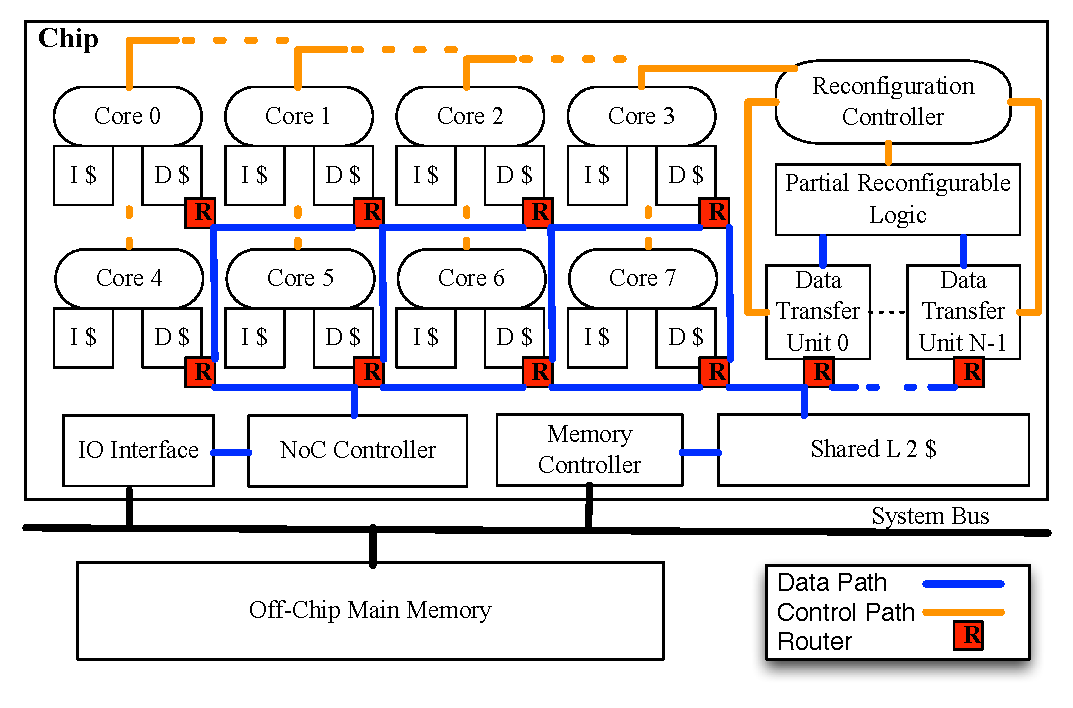
\includegraphics[width=4.0 in]{HPCA14-arch}
    \caption{Architecture Overview of {\em Transformer} }
    \label{fig_arch}
\vspace{-0.05in}
\end{figure}

The {\em Transformer}'s reconfigurable logic consists of the computational resources
and the {\em N} data transfer
units, which supports the instantiation of {\em N} independent accelerator
functions. The computational resources are organized in BRAM, DSP,
as well as SLICEs as in a generic FPGA chip. The actual number of functions instantiated within the
programmable logic depends on the particular functions selected to be
sped up at runtime and the resource requirements of the hardware
implementation for these functions. We study the architectural trade-offs of 
the reconfigurable logic and the number of cores in terms of performance
gains and power savings in Section \ref{sec_perf}.

Figure \ref{fig_reconfig_controller} depicts the three key components
in controlling the reconfiguration of the accelerator logic:
the reconfiguration controller, the reconfigurable logic and the data transfer
units. The reconfiguration controller is responsible for programming
new functions into the reconfigurable logic through new bit streams or
partial reconfiguration. By using the control and status registers to record the
status of the reconfiguration logic, the controller receives
instructions from the middleware running on one of the cores, tracks
demands for the various function calls, and makes decisions on what functions to accelerate and
when to accelerate them.

The reconfigurable logic consists of a static region, a Partial
Reconfigurable Region (PRR) and an Internal Configuration Access Port
(ICAP). The static region contains the necessary logic outside of the
accelerator PRMs, including the clock module, the interconnection interface and the
memory control interface. The PRR can be divided into smaller
sub-regions and configured on demand with different partial bit streams. ICAP is notified by the reconfiguration controller regarding
the type of accelerator 
%PRMs ({\bf FIXME all different PRMs are located in
%  their fixed addresses}) 
that should be configured and when it should start. In response, ICAP notifies
the controller with a ``resource full" or a ``(re)configuration done" message by
writing to the specific bits of the control registers.

Each data transfer unit includes a pair of input and output buffers
that can be filled or drained by a DMA engine. The DMA engine is
responsible for the bulk data transfers between the L2 cache and the
IO buffers, which are used as a form of scratchpad memory in order for the
reconfigurable logic to complete the necessary operations on the data. Other
parameters such as the memory addresses and the data size of the DMA
operations are passed by the reconfiguration controller. The TLBs on each
of the data transfer units are responsible for translating virtual
memory addresses into physical memory addresses.


\begin{figure}
    \centering
    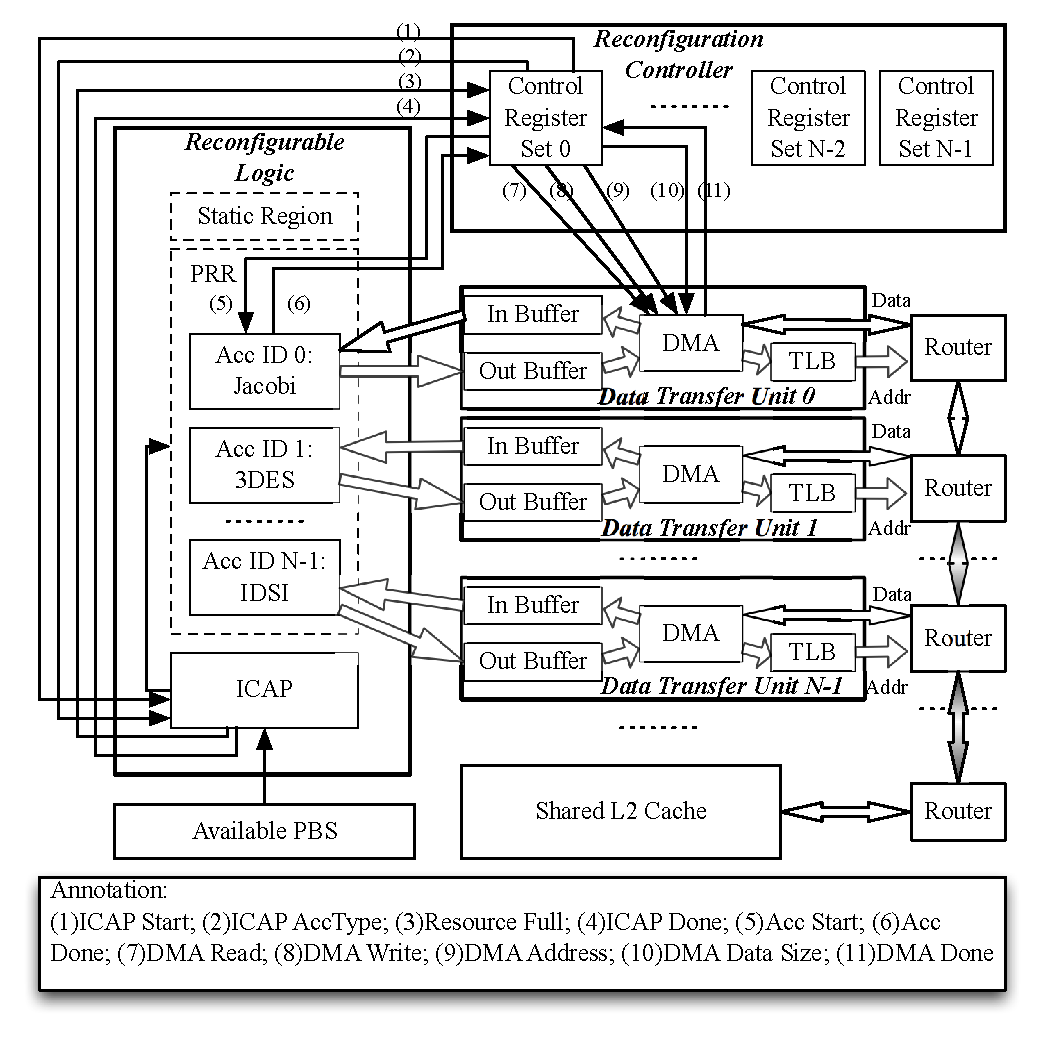
\includegraphics[width=4.0 in]{HPCA14-Controller}
    \caption{Transformer's Reconfigurable Logics and Controller}
    \label{fig_reconfig_controller}
\vspace{-0.05in}
\end{figure}


\subsection{Accelerator Invocation}

The invocation of the accelerator from the software executing within a given core is
done with specific accelerator instructions along with the control as well as the status
registers. We illustrate how the accelerator is invoked in Figure
\ref{fig_Acc_Invoc}. We introduce {\em N} control register sets for
each accelerator to be instantiated along with two new instructions to
invoke the core-to-accelerator as well as the accelerator-to-core execution path
transitions. Each control register set contains three 32-bit registers, including the
general control register, the DMA read register and the DMA write
register. The general control register is responsible for ICAP control,
acceleration control, and DMA control. The DMA read and write registers
contain the read and write addresses for the corresponding DMA operation source and destination
addresses. The specifications of the registers are described in Table
\ref{tbl_AccReg} while the two new instructions are listed below.

\begin{enumerate}
\item{\em readreg n}: read control register set with ID n.
\item{\em writereg n}: write the value into control register set with ID n.
%\item{\em accload AccReg n}: start configuring the type of accelerator
%  bitstream indicated by AccReg n into the reconfigurable logic. 
\end{enumerate}

\begin{table}[ht]
\scriptsize
\begin{center}
\begin{tabular}{|l|l|l|}
\hline 
\textbf{Register Name} & \textbf{Bits} & \textbf{Function}\\ 
\hline 
\hline
General Control &{\em Bit 0}   & ICAP start bit (IS)\\ 
\hline 
 &{\em Bit 1}   &  ICAP done bit (ID)\\ 
\hline 
 &{\em Bit 2-6} & ICAP accelerator type (IT 0-4)\\ 
\hline 
 &{\em Bit 7}   & acceleration start bit (AS)\\ 
\hline 
 &{\em Bit 8}   & acceleration done bit (AD)\\ 
\hline 
 &{\em Bit 9}   & DMA read enable (RE)\\ 
\hline 
 &{\em Bit 10}  & DMA write enable (WE)\\ 
\hline 
 &{\em Bit 11}  & DMA done (DD)\\
\hline
 &{\em Bit 12-15} & accelerator ID (ID 0-3)\\
\hline
 &{\em Bit 16-31} & DMA data block size (DS 0-15)\\
\hline
DMA Read Control &{\em Bit 0-31}  & DMA read address (RA 0-31)\\
\hline
DMA Write Control &{\em Bit 0-31} & DMA write address (WA 0-3)\\
\hline
\end{tabular} 
\caption{Control Registers for Reprogramming Accelerators.}
\label{tbl_AccReg}
\end{center}
\end{table}

The following is a brief introduction to intricacies of invoking the accelerator. 
Note that all the set and reset operations are done by using the
{\em readreg} and the {\em writereg} instructions. The aforementioned instructions are
encapsulated within customized wrapper functions, instead of being
used directly within a given user application.

\begin{enumerate}
\item If the reconfigurable controller decides to configure a specific
  combination of functions, based upon knowledge derived from the middleware, the
  middleware will set the ICAP Start (IS) bit in order to initiate the
  reconfiguration process using the corresponding functions identified by ICAP
  accelerator type (IT 0-4). (Note that the loading process will be skipped if
  the function is already configured within the accelerator logic.) At the
  same time, the middleware will prepare the data address and the data
  block size by writing the DMA read address (RA 0-31) bits and DMA
  data block size (DS 0-15) bits.

\item In addition to the reconfiguration process, we set the DMA Start
  (DS) bit in order to initiate reading data from the shared L2 cache or main
  memory into the accelerator local input buffer until the buffer is full.

\item When the reconfiguration is done, ICAP will set the ICAP Done
  (ID) bit to enable the start of the acceleration. By setting
  the acceleration start (AS) bit, the Reconfiguration Controller causes a
  thread context switch on the corresponding core, which begins the
  execution of a different thread. The suspended thread will sleep
  until the acceleration done (AD) bit is set.

\item When the acceleration function has completed or the middleware
  decides to erase and change the accelerator function for the core,
  the AccDone (AD) bit will be set and an interrupt will be generated in order to
  wake up the sleeping thread. Afterwards, the core will resume the previously
  inactive thread, which will either continue a software path or get
  ready for the next accelerator invocation.
\end{enumerate}


\begin{figure}
    \centering
    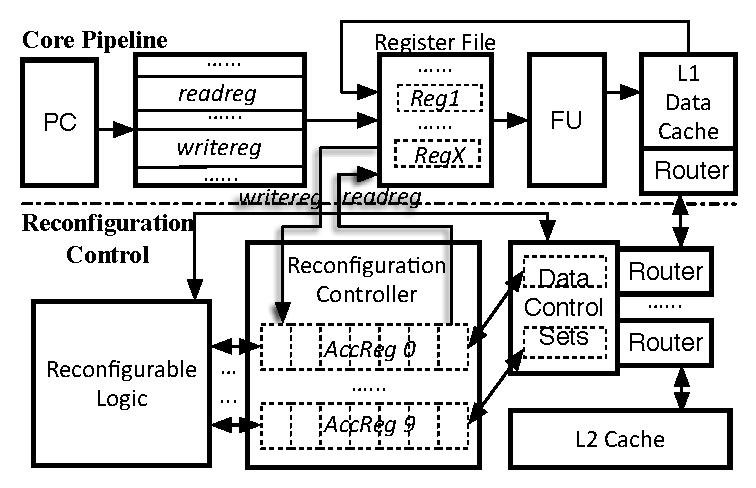
\includegraphics[width=4.0 in]{HPCA14-Acceleration_Invocation}
    \caption{Acceleration Invocation.}
    \label{fig_Acc_Invoc}
\end{figure}


In order to reduce the data transaction time between the accelerators, a
combination of DMA and double buffering is used. 
By using double buffering, the accelerators can work on data residing in
their local memory while the DMA is fetching the next batch of data. A
TLB is located in between the DMA cache as well as the L2 cache in order to perform
virtual-to-physical address translation. The aforementioned mechanism simplifies the
accelerator design and guarantees process isolation.


\section{Transparent Acceleration}
\label{sec_transacc}


Transparent acceleration of workloads is one of the design goals of
the {\em Transformer}. Transparent acceleration refers to the speedup of
an application using hardware accelerators without the need for source
code access, recompilation, or user intervention at run-time. We argue that such a feature is one of
the most important factors that enables the practical deployment of the
proposed heterogeneous architecture for the following reasons. 
First, the users'
workloads are typically present in the form of binary executables. The difficulties in obtaining access to the source code as well as 
rewriting the application impose tremendous obstacles for taking
advantage of the hardware accelerator. Second, the development environment
for user applications cannot be easily duplicated or emulated within
the run-time environment due to the complexity and variety of
the compilers as well as the libraries. As a result, the recompilation of an
application for hardware acceleration is either infeasible or
problematic. Third, recompilation of user applications introduces
delays which are often unnecessary and/or intolerable. Therefore
transparent acceleration is critical when applying hardware accelerators to unpredictable
workloads.

In order to achieve transparent acceleration and ease the work of programmers,
we focus on the acceleration of commonly used libraries such as
libopenssl. Such libraries are made available with well known APIs for
their core functions, and are often the targets of acceleration. For
example, 3DES, a classic block cipher, is one of the many functions
contained within libopenssl, which also includes a cryptography library implementing the Secure
Sockets Layer (SSL) as well as the Transport Layer Security
(TLS)\cite{wikissl} protocols. By taking on the form of a dynamically linked
library, libopenssl provides entry points for its functions, including
3DES. We propose to add a layer of wrapper functions that profile and
intercept the calls from user applications to the libraries, which can then
be accelerated through the use of programmable logic. 


\begin{figure}
    \centering
    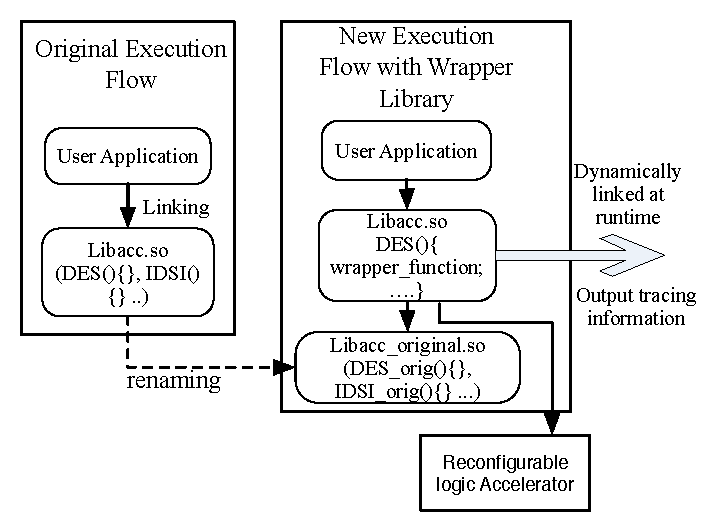
\includegraphics[width=4.0 in]{HPCA14-wrapperlib}
    \caption{Original and Modified Execution Flow}
    \label{fig_transacc_flow}
\end{figure}

Wrapper functions are presented in the form of dynamically linked
libraries, which utilize renaming in order to replace the original libraries. As a result,
the calls to the original dynamic library are directed to the wrapper
functions due to the linker stub \cite{linkerstub}. The modified
execution flow is shown in Figure \ref{fig_transacc_flow}.  The
original dynamically linked library is renamed by adding a suffix
{\em ``\_original''}.  The dynamically linked library functions are renamed by rewriting the corresponding symbol table. 
We create our new dynamic-linked library with the same name as the original library, and
incorporate a wrapper function to intercept all the library calls, specifically calls to the original function names, and
redirect them to either the original software library or the hardware
accelerator. As 
Section \ref{sec_perf} demonstrates, the wrapper library is
executed on a CPU core with a very small amount of overhead.

The responsibilities of the wrapper functions are two fold.
First, with regards to {\em profiling},
a wrapper library records the number of calls to each of the
library functions. Such counters reflect the demands on individual
functions, for example 3DES, which are used by the reconfiguration
controller to determine which functions are to be accelerated within the
programmable hardware. We provide details regarding the algorithms for the
run-time reconfiguration in Section \ref{sec_runtime_reconfig}.
Second, with regards to {\em function call redirection},
 a wrapper function directs the
execution flow to an appropriate path, either allowing the continuation of software instruction execution on a core or
accelerating software instruction execution within a programmable hardware unit. The wrapper functions
are aware of the currently accelerated functions on the programmable
accelerators, and such knowledge is updated by the reconfiguration
controller. If the required function is currently supported in the hardware
accelerator, this call and subsequent ones to the particular library
function(s) are redirected to the accelerator, thus reducing execution
time.

Library based transparent acceleration benefits dynamically
linked applications which are well supported in modern operating
systems, such as Windows and Linux. For statically linked applications,
although the dynamic library based transparent acceleration is limited
in detecting library calls and redirecting instruction flow to
hardware accelerators, we argue that such limitations are not inherent
within the context of the proposed heterogeneous architecture. A user can still
incorporate our wrapper functions into their applications so that any 
calls to compute-intensive functions will be appropriately instrumented.  Furthermore,
subsequent function calls are redirected to programmable accelerators after the
run-time system determines that the function should be sped
up with a hardware based accelerator.
We illustrate the process of a sample acceleration function call in Algorithm \ref{alg_sample_func}.

\begin{algorithm}[htb]
\scriptsize
\caption{Sample Acceleration Function Call}
\label{alg_sample_func}
\begin{algorithmic}[1]
\STATE {\em In User Function:}
\STATE {Call: DES (arg1, arg2, arg3) \newline}
\STATE {\em In Wrapper Function DES(arg1, arg2, arg3):}

\IF {DES is called}
	\STATE {RequestCounter ++ \COMMENT{Increase Request Counter by 1}}
	\IF {Request tracking time window is finished}
		\STATE{$D_{x} = \sum_{i=1}^{H}C(x,i)$ \COMMENT{Total demand}}
		\STATE{$DC_{x} = \sum_{i=1}^{H-1}(|C(x, i+1)-C(x, i)|)$\COMMENT{Demand changes}}
		\IF {Use naive scheduling}
			\STATE{$P_x = a \times D_x + (1-a) \times DC_x$ \COMMENT{Priority of this function}}
		\ENDIF
		\IF {Use Bandwidth/Speedup First scheduling}
			\STATE{$P_x = $ the result of 2D-knapsack combination}
		\ENDIF
	\ENDIF
	\IF {Function DES meets the requirement of being scheduled}
		\STATE{$ConfigStart \leftarrow 1$; $AccType \leftarrow 0$ \COMMENT{3DES is type 0}}
		\STATE {$ArgNum \leftarrow 3$; $AccPtr \leftarrow \& arg1$; $DS \leftarrow 1$}
		\IF {$ConfigDone = 1\quad\AND\quad DD = 1$}
			\STATE{$AccStart \leftarrow 1$}
		\ENDIF
		\IF {$AccDone = 1$}
			\STATE{Get back to previous thread.}
		\ENDIF
	\ELSE
		\RETURN $DES(arg1, arg2, arg3) \COMMENT{\text{Software  Version}}$
	\ENDIF
\ENDIF

\end{algorithmic}

\end{algorithm}










\section{Run-time Reconfiguration }
\label{sec_runtime_reconfig}

\subsection{Overview}
\label{subsec_runtime_reconfig_overview}

Run-time reconfiguration refers to the action taken by the controller
to make decisions on when to accelerate certain software libraries
based on run-time workload characteristics, and how to assess the
workloads periodically. The heart of reprogramming hardware
accelerators at run-time lies in the algorithms and mechanisms to
identify software functions to accelerate with the goals of sharing
the memory/logic resources and maximizing the resource utilizations of
reconfigurable logics. Since reprogramming the accelerator logic 
introduces a delay, we do not want the overheads of
reprogramming to outweigh the benefits of accelerating time-consuming
tasks. We propose a reconfiguration controller which addresses three
questions: (1) how to track the demands of candidate workloads; (2)
when to reprogram the acceleration logics; and (3) which accelerator
or combination of accelerators should be instantiated.


We answer these three questions in two steps:
(1) demand tracking and (2) request scheduling. As described in
Section \ref{sec_transacc}, in the first step we intercept all the
library calls with wrapper functions and keep track of the demands
using a table of counters called Request Counters (RC). The RCs
are regarded as a request log with updated information in the most
recent time window. In the second step, we apply heuristic algorithms to
schedule the requested function in hardware accelerators, and we
explain the algorithms in Section \ref{subsec_combo}. 

\subsection{Demand Tracking} 

The demands of computing a candidate function are tracked by the
wrapper function library. The library maintains a table of candidate
hardware accelerators and the functions that they speed up. Each call
to a function is intercepted and recorded by the wrapper function, and used as an
index to the table to increment the corresponding request counter. The
counters are input metrics to the scheduling algorithm to determine which
functions to accelerate. Tracking demands requires a table
lookup and a table update, i.e. only two memory operations (one
read and one write). The overheads of maintaining counters are trivial even when the number
of accelerators scales up to hundreds, this is because such counter
update is only once per a library function call, and the library function itself is typically very time-consuming (e.g. in millions of cycles). The counters
are reset periodically to record the most recent demands. 


At the presence of dynamic workloads and heterogeneous processing
elements (general-purpose cores and programmable accelerators), the
candidate functions to accelerate could be multiple and
time-dependent. The workload acceleration turns into an optimization
problem where the objective is to schedule tasks on multiple
processors for minimizing the execution time. As Hochbaum et
al. prove that similar scheduling on uniform processors is NP-hard
\cite{hochbaum88}, the scheduling on heterogeneous processing 
elements is also NP-hard. Therefore we derive heuristics to address
the remaining two questions: specifically we address question (2) with
the heuristics on determining the timing of reconfiguration in
Section \ref{subsec_ranking}, and question (3) with heuristics on
scheduling and combining accelerators in Section \ref{subsec_combo}.

\subsection{Request Ranking}
\label{subsec_ranking}

Each time when function acceleration requests are detected by the
wrapper library, we increment the corresponding request counter in a
time window of length $T$ before resetting it in the next window. 
We are not only interested in the number of calls within $T$, but also the {\em changes} in the demands
between subsequent time windows. This is because the dynamic workloads
could experience demand fluctuation, therefore historical trend in the
past time windows is as important as the number of calls in one or
multiple time windows.
Smaller $T$ leads to frequent counter resets and can trace the trend
of demands in a finer granularity, whereas large $T$ avoids
oversampling the demands and reprogramming the accelerators more
frequently than necessary. So the value of $T$ should be chosen
appropriately such that it does not add significant overheads when
comparing to the execution time of applications under study, and it is
enough to capture very detailed demand changes of acceleration
requests. 

We maintain an array of counters $C(x, i)$ collected in the past $R$
time windows, where $x$ represents the corresponding accelerator
function and $1<i<R$. At run time, we would have an $f \times R$
matrix $M$ that reflects the demands for $f$ accelerator functions in
the past $R$ time windows.  After obtaining $M$, we use the following
two metrics to evaluate the total demand $D_x$ and the rate of demand
changes $DC_x$ for every function $x$: $D_{x} = \sum_{i=1}^{H}C(x,i)$
and $DC_{x} = \sum_{i=1}^{H-1}(|C(x, i+1)-C(x, i)|)$.  The priority
$P_x$ of function $x$ is then calculated as $P_x = a \times D_x +
(1-a) \times DC_x$. We set $a$ as 0.5 in our implementation because we
regard the changes of demand as important as the total demands. $P_x$
is used to rank the accelerators requests in a descending
order. Changes in the ranking from the past time window trigger
reprogramming the accelerator functions in the on-chip logic. We regard this scheduling strategy as the baseline and denote it as ``na\"{\i}ve'' in the performance evaluation.

\subsection{Combining Accelerators}
\label{subsec_combo}



Combining acceleration functions to maximize the utilization of reconfigurable logic
allows for more effective speedup and power savings.

As each accelerator function consumes a certain amount of
on-chip resources such as the LUT, the memory, and the data access
bandwidth to achieve a particular speedup factor, as shown in Table
\ref{tbl_benchmark}, the choice of accelerators to maximize gains
under resource constraint is a combinatorial optimization problem, specifically the knapsack problem. 
We will discuss two variants to the knapsack problem
applicable in our accelerator scheduling algorithm.
The first is a 0-1 knapsack problem, specifically an acceleration function is either chosen or not
chosen.
The second is a bounded knapsack problem, where up to $n$ copies of
the same acceleration function can be instantiated as independent
engines into the accelerator. 
With the total resources available to the programmable accelerator as
one constraint, we consider two different prioritization strategies to minimize the
execution time, specifically the memory bandwidth utilization first strategy as well as the acceleration
speedup first strategy when solving the knapsack problems.

\subsubsection{Mathematical Model}

We model an accelerator function as $A(SLICE, DSP, BRAM, Bandwidth, Speedup)$,
where {\em SLICE, DSP, BRAM} are logic, application-specific blocks and
memory cell resources, respectively.  The aforementioned elements are consumed by the function when it is
instantiated in the reconfigurable logic unit. In the interest of minimizing the amount of time during which the unit remains idle, one
 requirement of the functions is to maximize the {\em bandwidth} of the data bus. {\em Speedup} is the effective speedup of an accelerated function on the reconfigurable logic compared to its software implementation. 

\begin{table*}[ht]
\scriptsize
\centering
\begin{center}
\begin{tabular}{|c|c|c|c|c|c|c|c|c|c|c|c|}
\hline 
\textbf{Accelerators}& \textbf{SLICE} & \textbf{SLICE \%} & \textbf{FF} & \textbf{FF \%} & \textbf{LUT} & \textbf{LUT \%} & \textbf{BRAM} & \textbf{BRAM \%} & \textbf{Bandwidth MB/s} & \textbf{Speedup} & \textbf{Power W} \\ 
\hline
\hline  
3DES          & 1148  & 24.7  & 807  & 8.7  & 1081 & 11.6  & 8    & 40   & 392   & 25.2     & 0.157\\ 
\hline 
IDSI          & 1637  & 35.2  & 530  & 5.7  & 891  & 9.6   & 0    & 0    & 970   & 13.1     & 0.235\\ 
\hline 
SLAM-C        & 812   & 17.4  & 973  & 10.4 & 854  & 9.2   & 0    & 0    & 479   & 33.0     & 0.156\\ 
\hline 
SLAM-J        & 983   & 21.1  & 1027 & 11.1 & 872  & 9.4   & 0    & 0    & 458   & 29.0     & 0.147\\ 
\hline 
SURF          & 1877  & 40.3  & 1163 & 12.5 & 705  & 7.6   & 5    & 25   & 983   & 25.0     & 0.161\\ 
\hline 
Segmentation  & 2918  & 62.7  & 930  & 10.0 & 630  & 6.8   & 12   & 60   & 848   & 45.5     & 0.178\\ 
\hline 
SmithWaterman & 626   & 13.4  & 1285 & 13.8 & 1034 & 11.1  & 20   & 100  & 403   & 36.6     & 0.182\\ 
\hline 
Jacobi        & 1201  & 25.8  & 1431 & 15.4 & 1218 & 13.1  & 2    & 10   & 1112  & 30.6     & 0.153\\ 
\hline 

\end{tabular} 
\caption{Benchmark accelerator logic cost, bandwidth, speedup and
  power {\em (Use Xilinx SPARTAN 3E as a reference)}} 
\label{tbl_benchmark}
\end{center}
\end{table*}

Table \ref{tbl_benchmark} summarizes the library functions under
study. The aforementioned library functions, explained in detail in \cite{accstore}, are
representative of time-consuming workloads relevant to a wide range of application
domains.  In the table, all data, excluding bandwidth consumption and
speedup, are derived from the open source synthesizable accelerator
store \cite{accstore}. We measure their memory bandwidth with the Intel
VTune Amplifier XE \cite{vtune}. The level of speedup for each accelerator is
calculated by dividing the execution time of one iteration of the software
benchmark on a 1.6 GHz single core by its corresponding hardware design
on a 200 MHz FPGA. The {\em Transformer} utilizes the Xilinx Spartan-3E XC3S500E
FPGA \cite{spartan3e} as a reference on-chip accelerator, which has a
comparable number of transistors, {$100\sim300$ million (500K gates)},
as eight Atom 330 cores, {$\sim 47$ million per core}
\cite{atom-spec}. The chip consists of a total number of 4,656 SLICE elements, 9,312 LUT elements
9,312, 9,312 FF elements, 768 DSP48 elements, and 20 BRAM elements. In addition, we indicate the
resource consumption percentage for each acceleration function. By
observation, the number of SLICE and BRAM elements serves as a significant
resource constraint. Therefore, we reduce the multi-dimensional
knapsack problem to a two-dimension problem. That is, we consider the
percentage of SLICE and BRAM elements for each benchmark as the two weights in
the knapsack model. The memory bandwidth utilization and level of speedup are
regarded as the two objective functions for reducing the total execution
time of memory-bound and compute-bound applications, respectively.

In the memory bandwidth-first combination, we attempt to maximize the
total bandwidth $\sum_{i=0}^{n}(BW_i \times Acc_i) $ subject to
$\sum_{i=0}^{n}(w_i \times Acc_i) $, where $Acc_i$ $i \in {1,2,3,
  ... ,n}$ denotes the different accelerator functions, $BW_i$ denotes the
bandwidth cost, and $w_i$ denotes their weight, that is the SLICE resource
demand. In the speedup-first combination selection, we focus our
efforts on maximizing the speedup metrics $\sum_{i=0}^{n}(SP_i) $, where
$SP_i , i \in {1,2,3, \ldots, n}$ denotes the speedup of each
accelerator. We attempt to maximize the two metrics by improving
the system bandwidth utilization and choosing a function with
 a significant level of speedup, which are two main approaches to improving system
performance. For example, our experiment results shows that if we
offload memory-bound benchmarks such as IDSI, SURF, Segmentation and
Jacobi to reconfigurable logics with higher memory bandwidth, we can
expect better overall performance and power efficiency. The aforementioned
heuristics are shown to be effective through extensive experimentation, which is
described further in Section \ref{sec_perf}.

\subsubsection{Dynamic Programming}

Both the two-constraint 0-1 knapsack problem and the two-constraint bounded knapsack problem can be solved
through the use of dynamic programming. 

\noindent{\em 0-1 Knapsack Problem Solution}

Assume we have $n$ acceleration functions to choose from, which are
annotated as $Acc_1$, $Acc_2$, \ldots, $Acc_n$. All $n$ items have
a two-constraint weight $a_i$, $b_i$ and a value $v_i$, $i \in [1,
  2, \ldots, n]$. We define $V[i, a, b]$ to be the current
maximum value we can obtain with a weight less than or equal to $a$
and $b$ using first $i$ accelerators. The upper limit of the two weights
are $A$ and $B$. We derive recursive equations for $V[i, a, b]$:

\begin{equation}
V[i, a, b] = V[i-1, a, b] \quad \text{if} \quad a_i > a, b_i > b,
\end{equation}
implying that if adding a new accelerator exceeds the current
two-dimensional weight limit, then we do not choose the new
accelerator and the total value will not change. As a result
\begin{equation}
\begin{array}{c}
	V[i, a, b] = max(V[i-1, a, b], V[i-1, a - a_i, b - b_i] + V[i, a, b])\\
	\text{if} \quad a_i \leq a \quad b_i \leq b.
\end{array}
\end{equation}

Algorithm \ref{alg:0-1-knapsack} describes how we solve the two-constraint 0-1
knapsack problem in order to select a set of accelerator functions. 

\begin{algorithm}[htb]
\scriptsize
\caption{ 0-1 Knapsack Problem Solution}
\label{alg:0-1-knapsack}
\begin{algorithmic}[1] 
\FOR {each $a \in [0, A]$}
	\FOR {each $b \in [0, B]$}
    	\STATE $ V[a, b] = 0; $
    \ENDFOR
\ENDFOR
\FOR {each $i \in [1, n]$ } 
    \FOR {each $a \in [A, a_i]$ }
    	\FOR {each $b \in [B, b_i]$}
    	
        	\IF {$j \geq w[i]$}
            	\STATE $V[i, a, b] = max(V[i-1, a, b], V[i-1, a - a_i, b - b_i] + v[i, a, b]) $
        	\ELSE
            	\STATE $V[i, a, b] = V[i-1, a, b]$
        	\ENDIF
        \ENDFOR
    \ENDFOR
\ENDFOR
\end{algorithmic}
\end{algorithm}

\noindent{\em Bounded Knapsack Problem}

The two-constraint bounded knapsack problem can be solved in a similar
way as the 0-1 knapsack problem. Utilizing two extra annotations, $C$, which represents the
maximum number of acceleration functions that we can request for a certain
function, and $k_i$ as the number of functions $i$ we can choose, 
 similar recursive equation can be derived for $V[i, w]$.

\begin{equation}
V[i, a, b] = V[i-1, a, b] \quad \text{if} \quad a_i > a, b_i > b
\end{equation}

and

\begin{equation}
	\begin{array}{c}
		V[i, a, b] = max(V[i-1, a, b], V[i-1, a - k_i\times a_i, b - k_i\times b_i] \\
		+ k_i\times V[i, a, b])\\
		\text{if} \quad a_i \leq a \quad b_i \leq b
	\end{array}
\end{equation}

The algorithm for the bounded knapsack problem is similar to Algorithm
\ref{alg:0-1-knapsack}, and is not elaborated further due to spacial limitations.





\begin{flushright}

\end{flushright}\section{Performance Evaluation}
\label{sec_perf}
 

\subsection{Simulator Overview}
To evaluate the performance and power consumption of the proposed
architecture, we simulate the multi-core heterogeneous architecture
by extending Multi2Sim - a superscalar, multithreaded and multicore
simulator - with a reconfigurable accelerator unit. 
 The specification of our simulated architecture is shown in Table
\ref{tbl_parameters}. The processor core technology and operating
frequency are modeled based on the Atom 330 processor. We set the
number of cores to be eight in the baseline configuration. Afterwards, we vary the
number of cores to explore the area allocation to the accelerators as well as the cores. 
The ICAP interface runs at 100 MHz, although over-clocking ICAP is
possible in practice \cite{Hansen:2011dt}.

\begin{table}
\scriptsize
\begin{center}
  \begin{tabular} { | l | l | }
    \hline
    \textbf{Item} & \textbf{Parameter} \\
    \hline
    \hline
	Core & 8 \\
	\hline
	Core Spec & 45nm @ 1.6 GHz \\
	\hline
	Accelerator Spec & 45nm @ 200 MHz \\
	\hline
	ICAP & 32 bit bus width @ 100 MHz \\
	\hline
	L1 Instr/Data \$ Size (KB) & 32 \\
	\hline
    L1 Instr/Data \$ Associativity & 4\\
    \hline
    L1 Instr/Data \$ Block Size (Bits) & 64\\
    \hline
    L1 Instr/Data \$ Number of Sets & 128\\
    \hline
    L1 Instr/Data \$ Latency (Cycles) & 3 \\
   	\hline
   	L2 Cache Size (MB) & 4 (shared) \\
   	\hline
    L2 Associativity & 8\\
    \hline
    L2 Block Size (Bits) & 512\\
    \hline
    L2 Number of Sets & 1024 \\
    \hline
    L2 Latency (Cycles) & 20\\
    \hline
    CPU Cache Coherence & MOESI\\
    \hline
    Accelerator Data Buffer Size (KB) & 8 \\
    \hline
    Accelerator Data Buffer Coherence & MOESI\\
    \hline
    Memory Size (GB) & 8 \\
    \hline
    Memory Latency (Cycles) & 200 \\
    \hline
    Memory Data Block Size (Bytes) & 512\\
    \hline
    Memory Page Size (Bytes) & 8192\\
    \hline
    Memory Replacement Policy & Pseudo LRU\\
    \hline
    Network Topology & 2-D Mesh\\
    \hline
    Network Bandwidth (MB/s) & 1024\\
    \hline
  \end{tabular}
\caption{Hardware Specification}
\label{tbl_parameters}
\end{center}
\end{table}


To model the profiling and scheduling overheads within the simulations,
we evaluate the overhead of the profiler in the wrapper function and the
three scheduling methods: na\"{\i}ve, bandwidth-first, or speedup-first. For
the worst case, the profiler and the wrapper function's overhead takes up
to 0.017 \% per profiling window.  The worst case occurs only
when the reconfiguration controller accepts the current acceleration
request within the profiling window. The two knapsack combination
scheduling algorithms introduce more overhead than the na\"{\i}ve scheduling. However, further evaluation shows that the overhead of both the bandwidth-first and the speedup-first algorithms introduce a neglectable overhead of 0.130 \% per profiling window. 

\subsection{Benchmarks}
We use all eight acceleration functions from the
open-source accelerator store \cite{accstore} to build a synthetic
workload that simulates the dynamic workloads within cloud and mobile
environments.  In this case, we defer using real-world cloud applications to our
future work.  These applications cover a wide range of areas
including encryption/decryption ({\em 3DES} \cite{openssl}), numerical
calculation ({\em Jacobi} \cite{jacobi-wiki}), vision and navigation
({\em SLAM-C and SLAM-J} \cite{openslam}), feature detection ({\em SURF} and
{\em IDSI} \cite{opencv}), image processing ({\em Segmentation}
\cite{segmentation-wiki}) and bioinformatics ({\em Smith-Waterman}
\cite{smithwaterman-wiki}). Moreover, the aforementioned software applications have
corresponding accelerator implementations which provide
performance as well as area allocation details. Minor modifications were done in order to generate the
final benchmark mixture, including preparing the input data set for
each function as well as the creation of multiple threads.

To emulate the dynamics of workload arrival, we model the inter-arrival time between
each benchmark as a Poisson distribution. The average
inter-arrival time is set to 500 million cycles, 312.5 ms
in real time if the system is running at 1.6 GHz, which in turn is close to the
cycle time of one iteration for our shortest benchmark IDSI. We compare
the Poisson arrival pattern with the default pattern of continuous
arrival, where the inter-arrival time is zero.

\subsection{Modeling Accelerators}
As there is no accelerator modeled in the stock Multi2Sim simulator,
 a general purpose core is modified to simulate a reconfigurable
accelerator unit. A best effort is made to model the
computation, the memory access, along with the reconfiguration delays based
upon prior work as well as our own benchmark studies. 

We model the timing of each accelerator by using their different
speedup values reported in the prior work as listed in Table
\ref{tbl_benchmark}. The speedup numbers are scaled to the 
operating frequencies for each core core as well as the reconfigurable logic used in our
simulations. 

We are interested in understanding the memory access
patterns, specifically the footprint, the data size and the frequency.  Furthermore, we are interested in modeling
the patterns within the accelerators using a series of high fidelity simulations. Towards this end, we profile the memory
activities by logging the memory access traces for each 
acceleration function.
Figure \ref{fig_mem_access} illustrates the memory access pattern for
two benchmark applications: Jacobi and SLAM-J. The horizontal axis represents
the time of the access, while the vertical axis represents the address within a given 
page range. In this way, we observe the temporal and spatial
characteristics of the memory accesses. It can be seen that {\em
  Jacobi} has larger number of accesses and that the
accesses span a wider address range. We model similar memory
access patterns when simulating the accelerators.  In addition, we visually
differentiate memory bound applications from computationally intensive
applications. 

The overhead of a DMA transfer is modeled within the approximation
formula derived from \cite{Saidi:2012}: $ T(s) = I + \alpha \times b \times
s$, where $I$ is the fixed initial cost, which includes issuing commands
along with the TLB translation, $\alpha$ is the transfer cost rate in
$cycles/byte$, $b$ is the basic block size, and $s$ is the super block
size. Given that the DMA command along with the TLB translation are already modeled separately within the wrapper libraries and
the stock Multi2Sim simulator, $I$ is set to 0 in this case. We choose $\alpha$
to be 2 cycles/byte as an average number \cite{Saidi:2012}. The variables $b$ and $s$
are to be determined by the appropriately relevant functions.


\begin{figure}
    \centering
    \includegraphics[width=6.0in]{Mem-Access}
	\caption{Memory access pattern of Jacobi (left) and SLAM-J (right)}
\label{fig_mem_access}
\end{figure}


The IO buffers on each of the accelerators are modeled by
modifying the Multi2Sim cache models. In this case, the MOESI cache coherence
protocol remains effective. The TLBs are employed to handle the virtual memory
address translation.  We have studied the impact of the size of the IO
buffers on the performance of the {\em Transformer}'s reconfigurable
logic. The results, which are not depicted here, reveal that the performance of
the accelerator increases significantly from 8KB to 32KB, beyond which no
substantial improvement is observed. As a result, our simulations use 32KB as
the default buffer size.

The partial reconfiguration delay $T_R$ is modeled as $ T_R = \frac{S_{pbs}}{ B_{ICAP} / C_{ICAP}} $,
where $S_{pbs}$ is the size of
partial bitstream, and $B_{ICAP}$ and $C_{ICAP}$ are the bus bandwidth
as well as the cycle time for ICAP.
Since the partial reconfiguration time depends on the size of the partial bit
stream, we conservatively model the reconfiguration time using the
largest bitstream size observed amongst all of the benchmarks within our simulations. 


\subsection{Power Model}
The dynamic and static power consumption of the general purpose cores are
estimated by using HP McPat v0.8 \cite{mcpat}. The power consumption of the reconfigurable logic
is modeled as follows. We track the number of
logic elements used by the accelerator functions at run time, 
including the number SLICE, FF, DSP48, and BRAM elements. The number of each logic element type serves as the input data to the 
Xilinx Power Estimator
\cite{xpe}, which serves to calculate the reconfigurable logic's power consumption.  
We scale the power of the reconfigurable logic to the 45 nm technology scale
so that both the cores and the accelerators are at the same technology
level. The total power consumption is the sum of the power of
the reconfigurable logic as well as the power reported by McPat for each of the
cores. 


\subsection{Simulation Results}
\label{sec_simu_result}

\subsubsection{Speedup of Multiple Copies of a Single Workload}

We first study the effectiveness of the {\em Transformer} on single function 
workloads. A software thread repeatedly executes a single function, such as the 3DES function,
 and then we gradually increase the number of threads. In this setting, both 
scheduling methods will select the same accelerator since the wrapper function
intercepts only one kind of library call. As a result, we only compare the architectures with
or without accelerators. 
Figure \ref{fig_num_of_apps} displays the performance speedup on the y
axis while the x axis displays the number of threads. The
baseline performance is the execution time for the $k$ threads on a multicore
architecture without an accelerator. We 
observe that the speedup for the 3DES function is significant, $\sim14\times$, when the number of threads is
approximately two, beyond which the speedup decreases. In this case the
resources available within the accelerator logic only allows up to two
3DES accelerator functions to be instantiated. The remaining threads
are executed as software within the cores.  As a result, the level of speedup is not
as significant as the ones observed within the earlier cases.  Other functions
experience similar trends but the number of acceleration function
copies differs from benchmark to benchmark.   

The disparity in the reconfigurable resource requirements among benchmarks
validates the observed opportunities for combining accelerators. Further
analysis indicates that the 3DES accelerator function requires 40\% of 
the BRAM resources of the reconfigurable logic, so that only two copies of
3DES functions can be instantiated. However, other types of
resources such as the LUT remain abundant when accommodating
functions such as SLAM-C, which requires only 9.2\% of the LUTs and none of the
BRAMs. Below, we illustrate the run-time accelerator instantiation and combination within Figure
\ref{fig_acc_timeline}.   

\begin{figure}
    \centering
    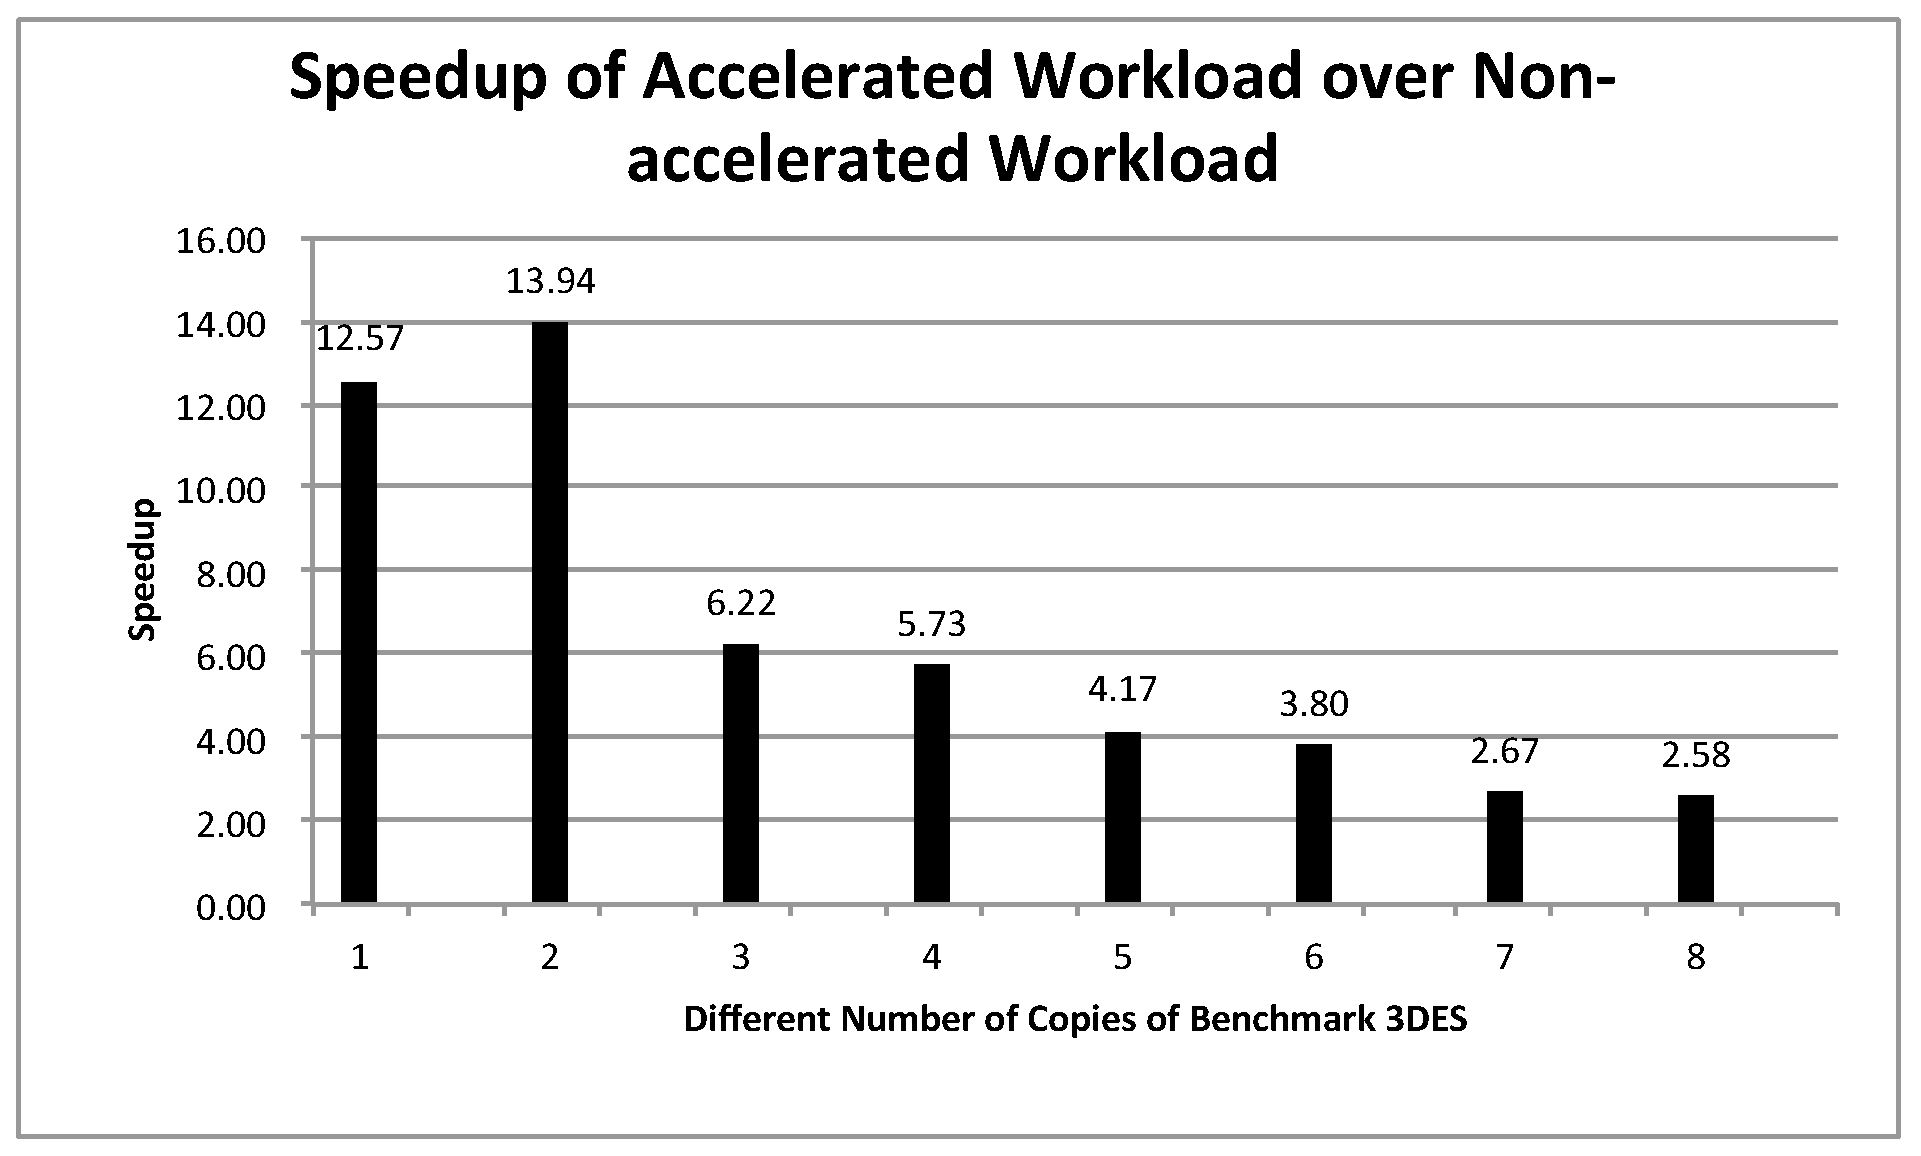
\includegraphics[width=4.5in]{Increase-Num-of-Apps}
    \caption{Speedup of Multiple Copies of a Single Workload Type}
    \label{fig_num_of_apps}
\end{figure}

\subsubsection{Speedup and Energy Efficiency of Workload Mixtures}

Given a mixture of the workloads, the instantiation of accelerator
functions is subject to the run-time demands as well as the constraints of the logic resources.
 We execute the synthetic workloads on the {\em Transformer} with eight
cores and one reconfigurable logic unit, which in this case matches the size of one Xilinx
Spartan 3E FPGA. The workload's arrival either follows a Poisson distribution or
a continuous back-to-back distribution. We issue 100 thousand billion instructions of
the benchmark bundle and record the number of completed functions as well as the
cycle times. 

\begin{figure}
    \centering
    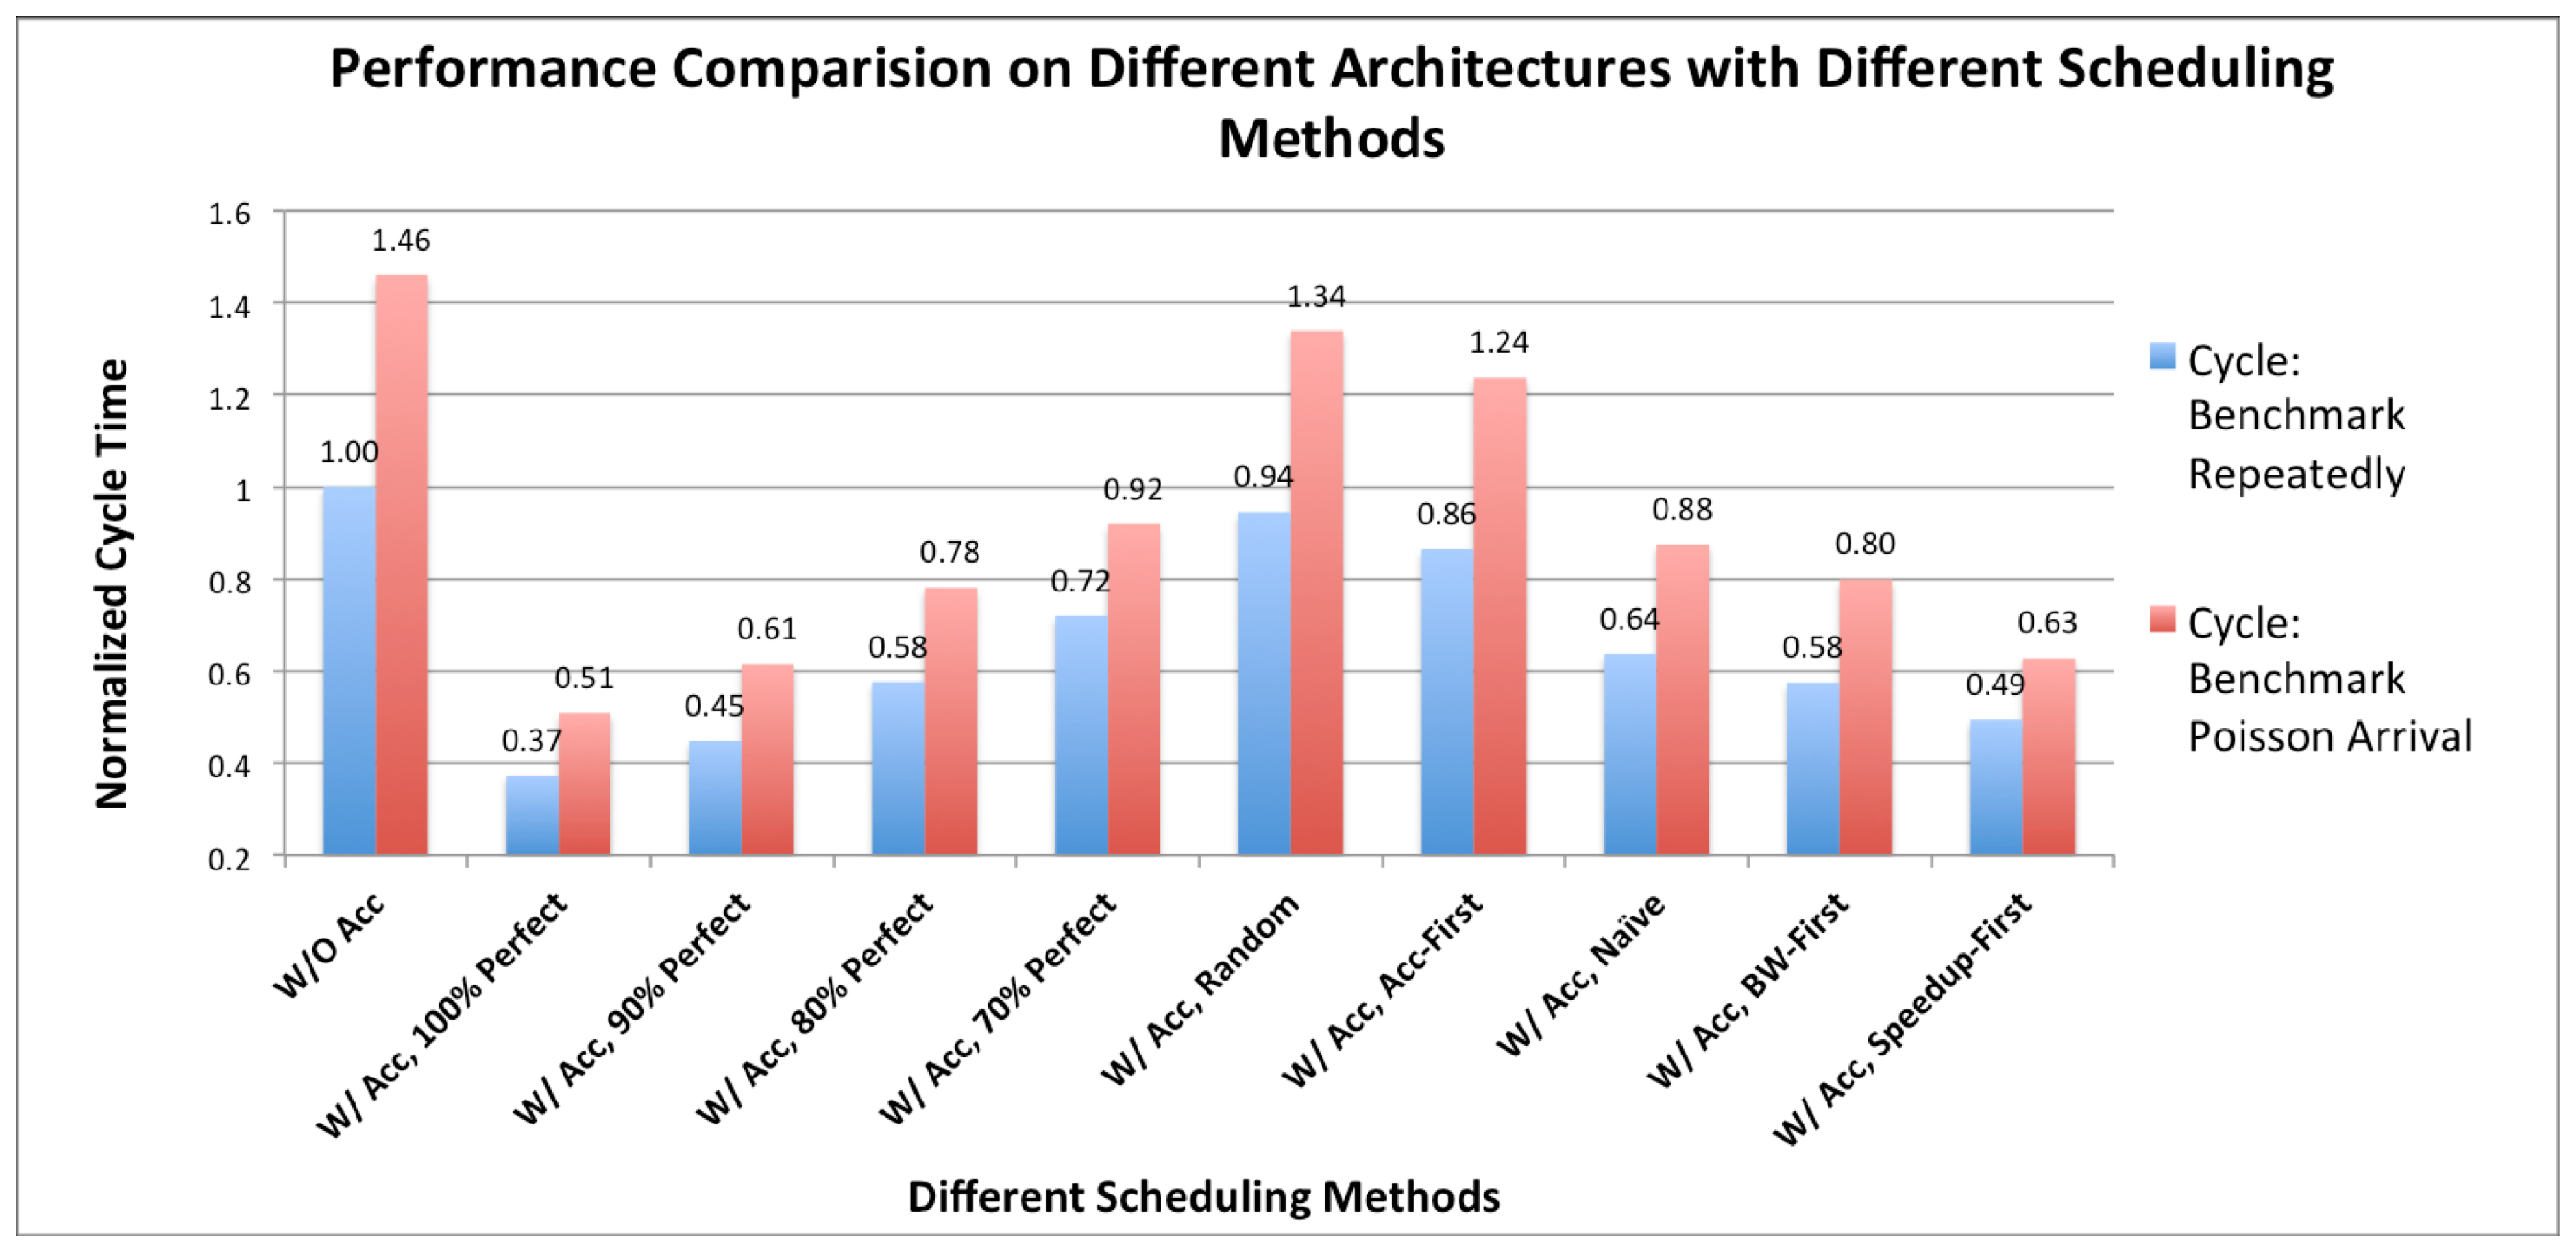
\includegraphics[width=4.5in]{Cycle-8core}
    \caption{Performance Comparison of Accelerated Architecture and Scheduling Algorithms}
    \label{fig_8core_cycle}
\end{figure}

\begin{figure}
    \centering
    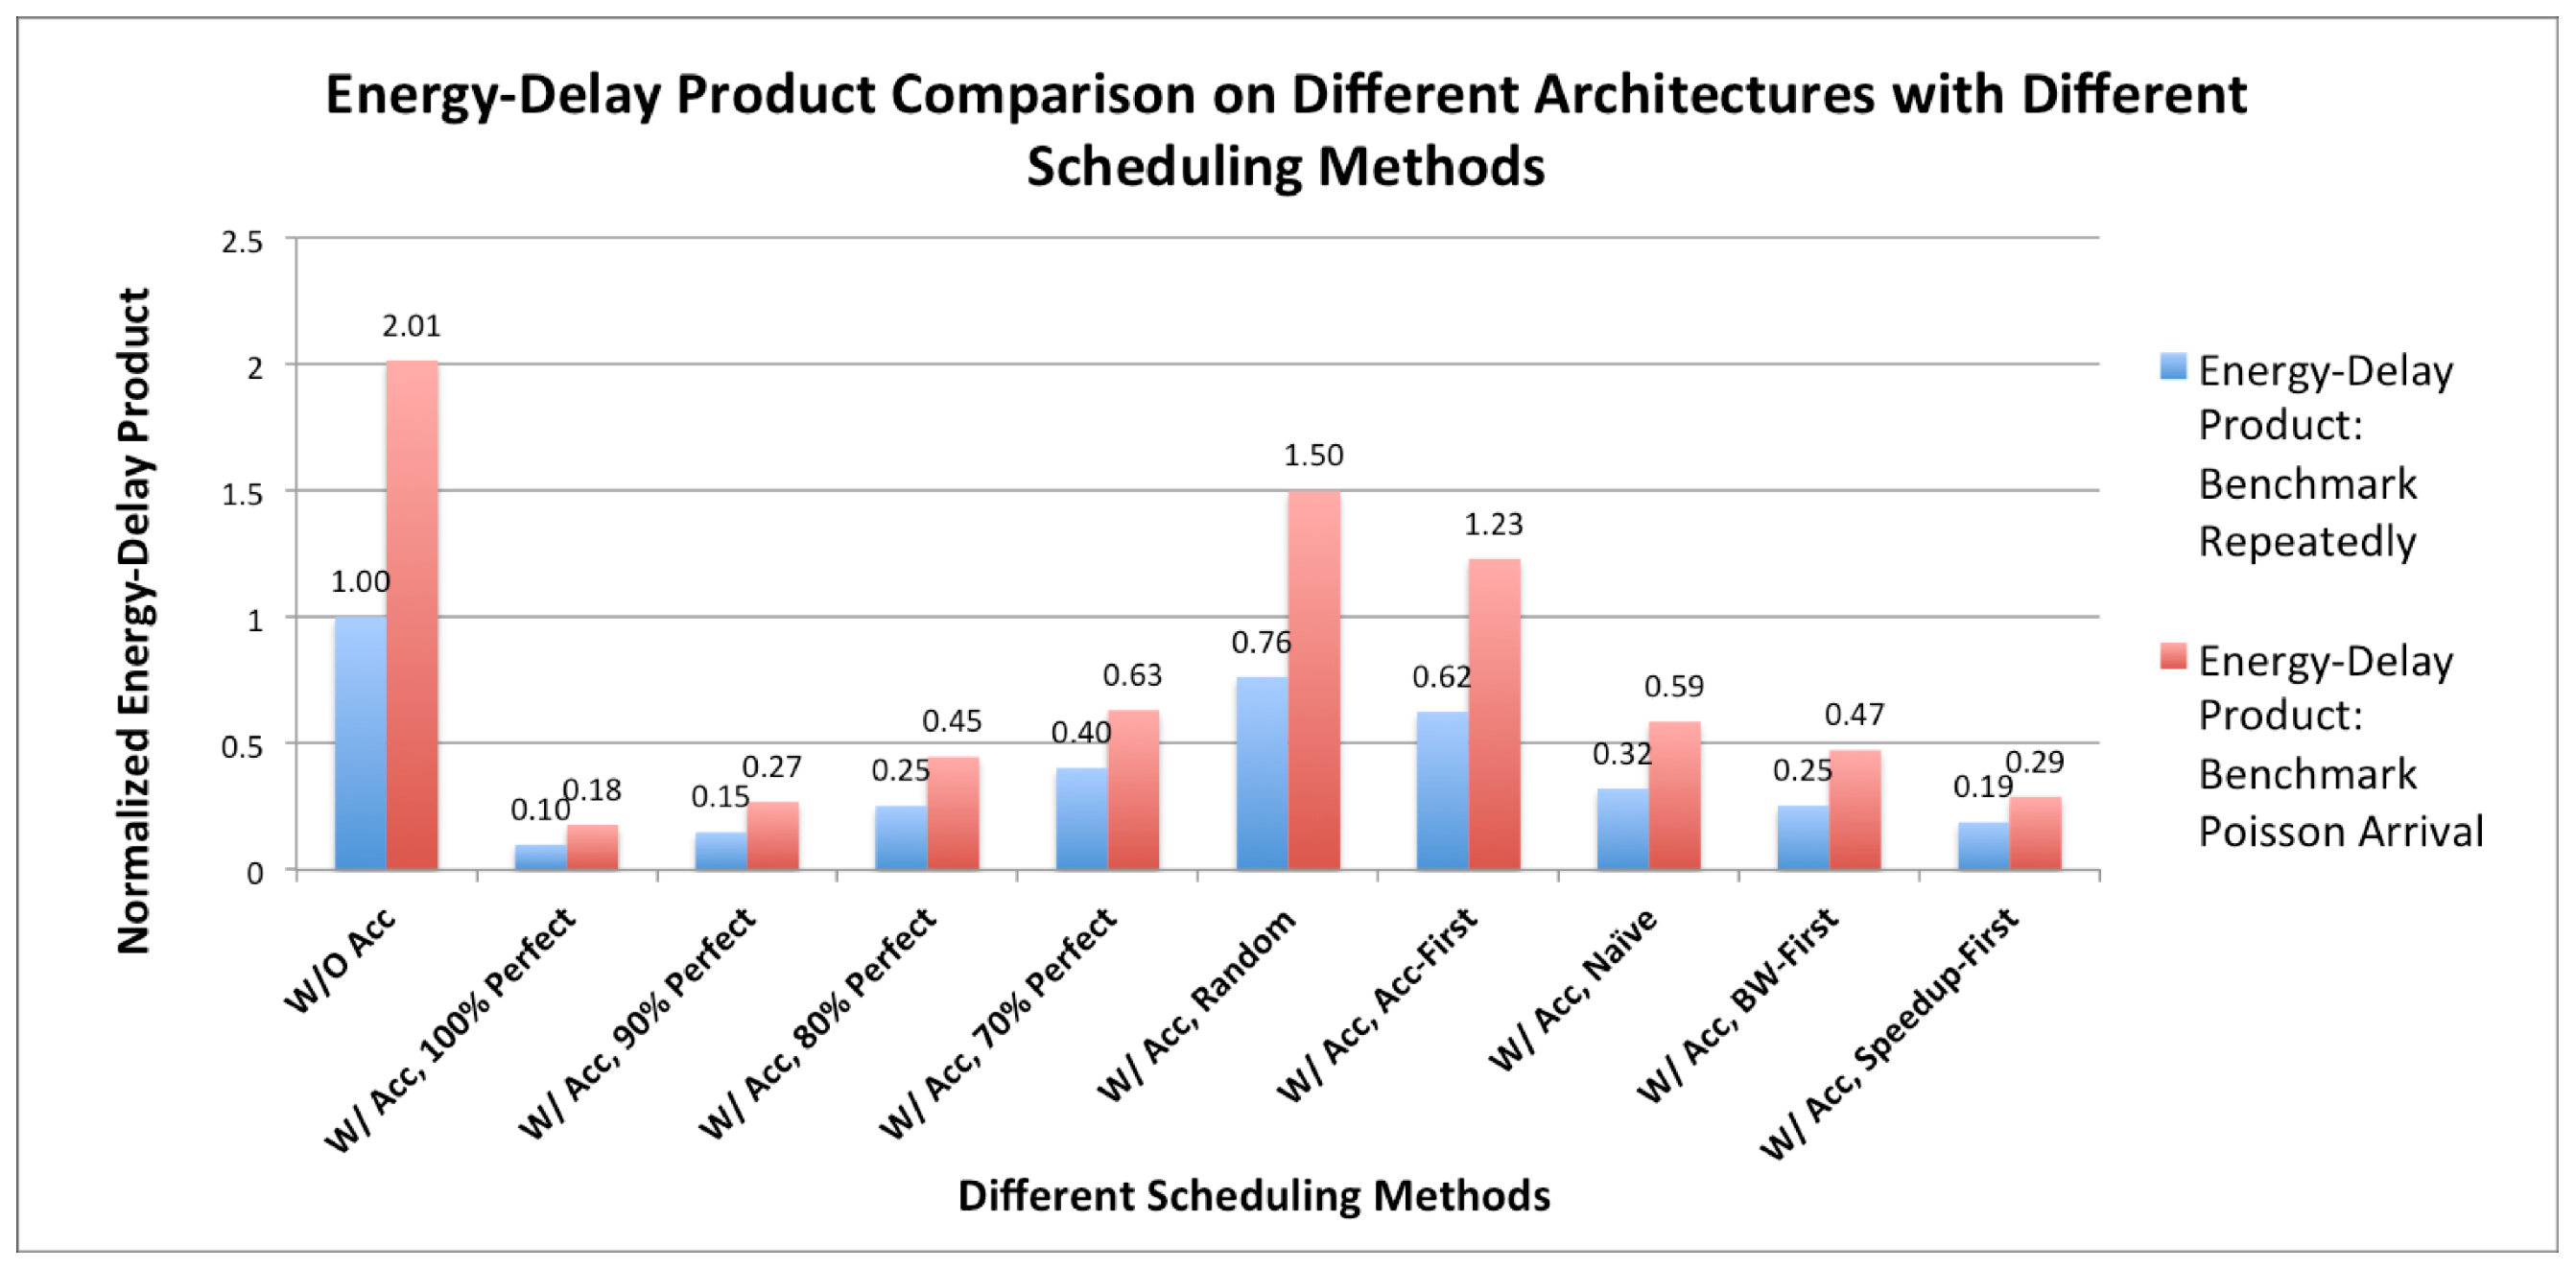
\includegraphics[width=4.5in]{Energy-Delay-8core}
    \caption{Energy-delay Product Comparison}
    \label{fig_8core_energy_delay}
\end{figure}

Figure \ref{fig_8core_cycle} depicts the performance of different
scheduling methods. The x-axis denotes different
architectures as well as scheduling methods, including:
 no accelerator, ``W/O Acc",
 with the accelerator and 100\% perfect prediction accuracy of the incoming workloads, ``W/ Acc, 100\% Perfect",
 with the accelerator and randomly scheduled incoming workloads to either the CPU or the accelerators, ``W/ Acc, Random",
 with the accelerator and the workload scheduled to accelerators with first priority, ``W/ Acc, Acc-First",
 with the accelerator and only profiling used, ``W/Acc, Naive", 
 with the accelerator and profiling plus bandwidth-first scheduling, ``W/ Acc, BW-First",
 with the accelerator and speedup-first scheduling ``W/ Acc, Speedup-First"
 The y-axis displays the normalized execution time.

The accelerated architectures deliver a factor of up to $2.3\times$ improvement in terms of performance as 
compared with a multicore architecture without an accelerator. It is
worth noting that the aforementioned speedup was achieved with a highly dynamic
workload bundle for which the processor has no prior knowledge of the
workload types or the arrival times. All the profiling is done at run-time and the
scheduling of the accelerator is autonomously performed by the
middleware wrapper library. The workload following a Poisson distribution
 resulted in a longer execution time as a result of the idle cycles
between each of the function calls. However, the Poisson distribution provides for dynamic
 combinations of workload arrival times, resulting in a
 larger observed speedup, $1.46/0.63\simeq2.3\times$, as compared with the
back-to-back arrival, $1/0.49\simeq2\times$. 

The energy-delay product depicted in Figure
\ref{fig_8core_energy_delay} indicates that the power efficiency of the {\em
 Transformer} produces an improvement up to ($2.01/0.29\simeq6.9\times$) as the workloads migrate to
the energy efficient accelerators resulting from the scheduling along with the run-time
reprogramming.



In comparison with other scheduling methods, we find ours
to be closely aligned with ``Perfect Prediction'' scheduling. In theory, the perfect
prediction scheduling scheme precisely predicts
the demands on the system based upon the incoming workloads. The aforementioned best possible scheduling
strategy provides us with the best performance and power
efficiency that is achievable with the given hardware. We see that our proposed speedup-first, bandwidth-first scheduling heuristic can
 achieve similar performance, in terms of execution time, as well as an energy-delay-product, with ``90\% Perfect'' scheduling and 
``80\% Perfect'' scheduling, respectively. The detailed
results are depicted in Figures \ref{fig_8core_cycle} and \ref{fig_8core_energy_delay}.  

\if 0
For example, the speedup-first scheduling method outperforms the
Random scheduling and Acc-First scheduling with a speedup of 2.12 and
1.96 respectively and a energy-delay factor gain of 5.17 and 4.24
respectively. The results of Perfect Prediction scheduling are
promising, however such ``perfect" prediction never happens with the
huge dynamics of the workloads in real world. Though ``perfect" in
prediction, the Perfect Prediction scheduling method does not yield
``perfect" utilization of the accelerator logic. 
As we argued in Section \ref{subsec_combo}, maximizing the utilization of reconfigurable logic is one of the contributions in our work to improve system performance and decrease the power consumption. The bandwidth-first scheduling and the speedup-first scheduling, on the contrary, take both accelerator size and performance gain into consideration. Thus, on one hand, bandwidth-first and speedup-first scheduling methods may not be able to compete with the 100\% Perfect Prediction in terms of the prediction accuracy, however on the other hand, their accelerator combination mechanism improves the whole system performance. As shown in Figure \ref{fig_8core_cycle}, speedup-first scheduling resembles the performance of the 90\% Perfect Prediction scheduling and bandwidth-first scheduling matches with the performance of 80\% Perfect Prediction scheduling. 
\fi

\subsubsection{Performance and Power Analysis with Various Time Window Sizes}

One of the basic parameter setups of the experiment is the choice for the profiling time window $T$. As we mention in \ref{subsec_ranking}, 
an inappropriate choice for the value of $T$ will result in either oversampling or inaccuracy. 
Thus, we implement a series of experiments in order to find the optimal value for $T$, one which can be used for our benchmarks. 
We take the non-accelerated scenario as our baseline. In addition, we compare the performance and power efficiency gain of the
 naive scheduling algorithm over the baseline case with different values for the profiling time window size. 
The experiment results are shown in Figure \ref{fig_time_window}.

The performance and the power efficiency increases as $T$ increases
from $1 ms$ to $100 ms$. Furthermore, the performance and the power efficiency plateau as $T$ remains between
 $100 ms$ to $1000 ms$.  In addition, the performance and the power efficiency decrease dramatically as $T$ increases beyond
$1000 ms$. The observed drop is the result of a loss in accuracy within the profiling
method as the benchmarks are down-sampled. According to the results, the range 
$[10 ms, 1000 ms]$ results in an acceptable value for $T$ within our
experiment. We thus set the window size $T$ to be $100 ms$.
%We also notice that the performance gain and power
%efficiency gain is still positive when $t = 1 ms$ tough sampling rate
%is the highest. That means the benefits of applying profiling and scheduling outweigh the profiling overhead. 

\begin{figure}
    \centering
    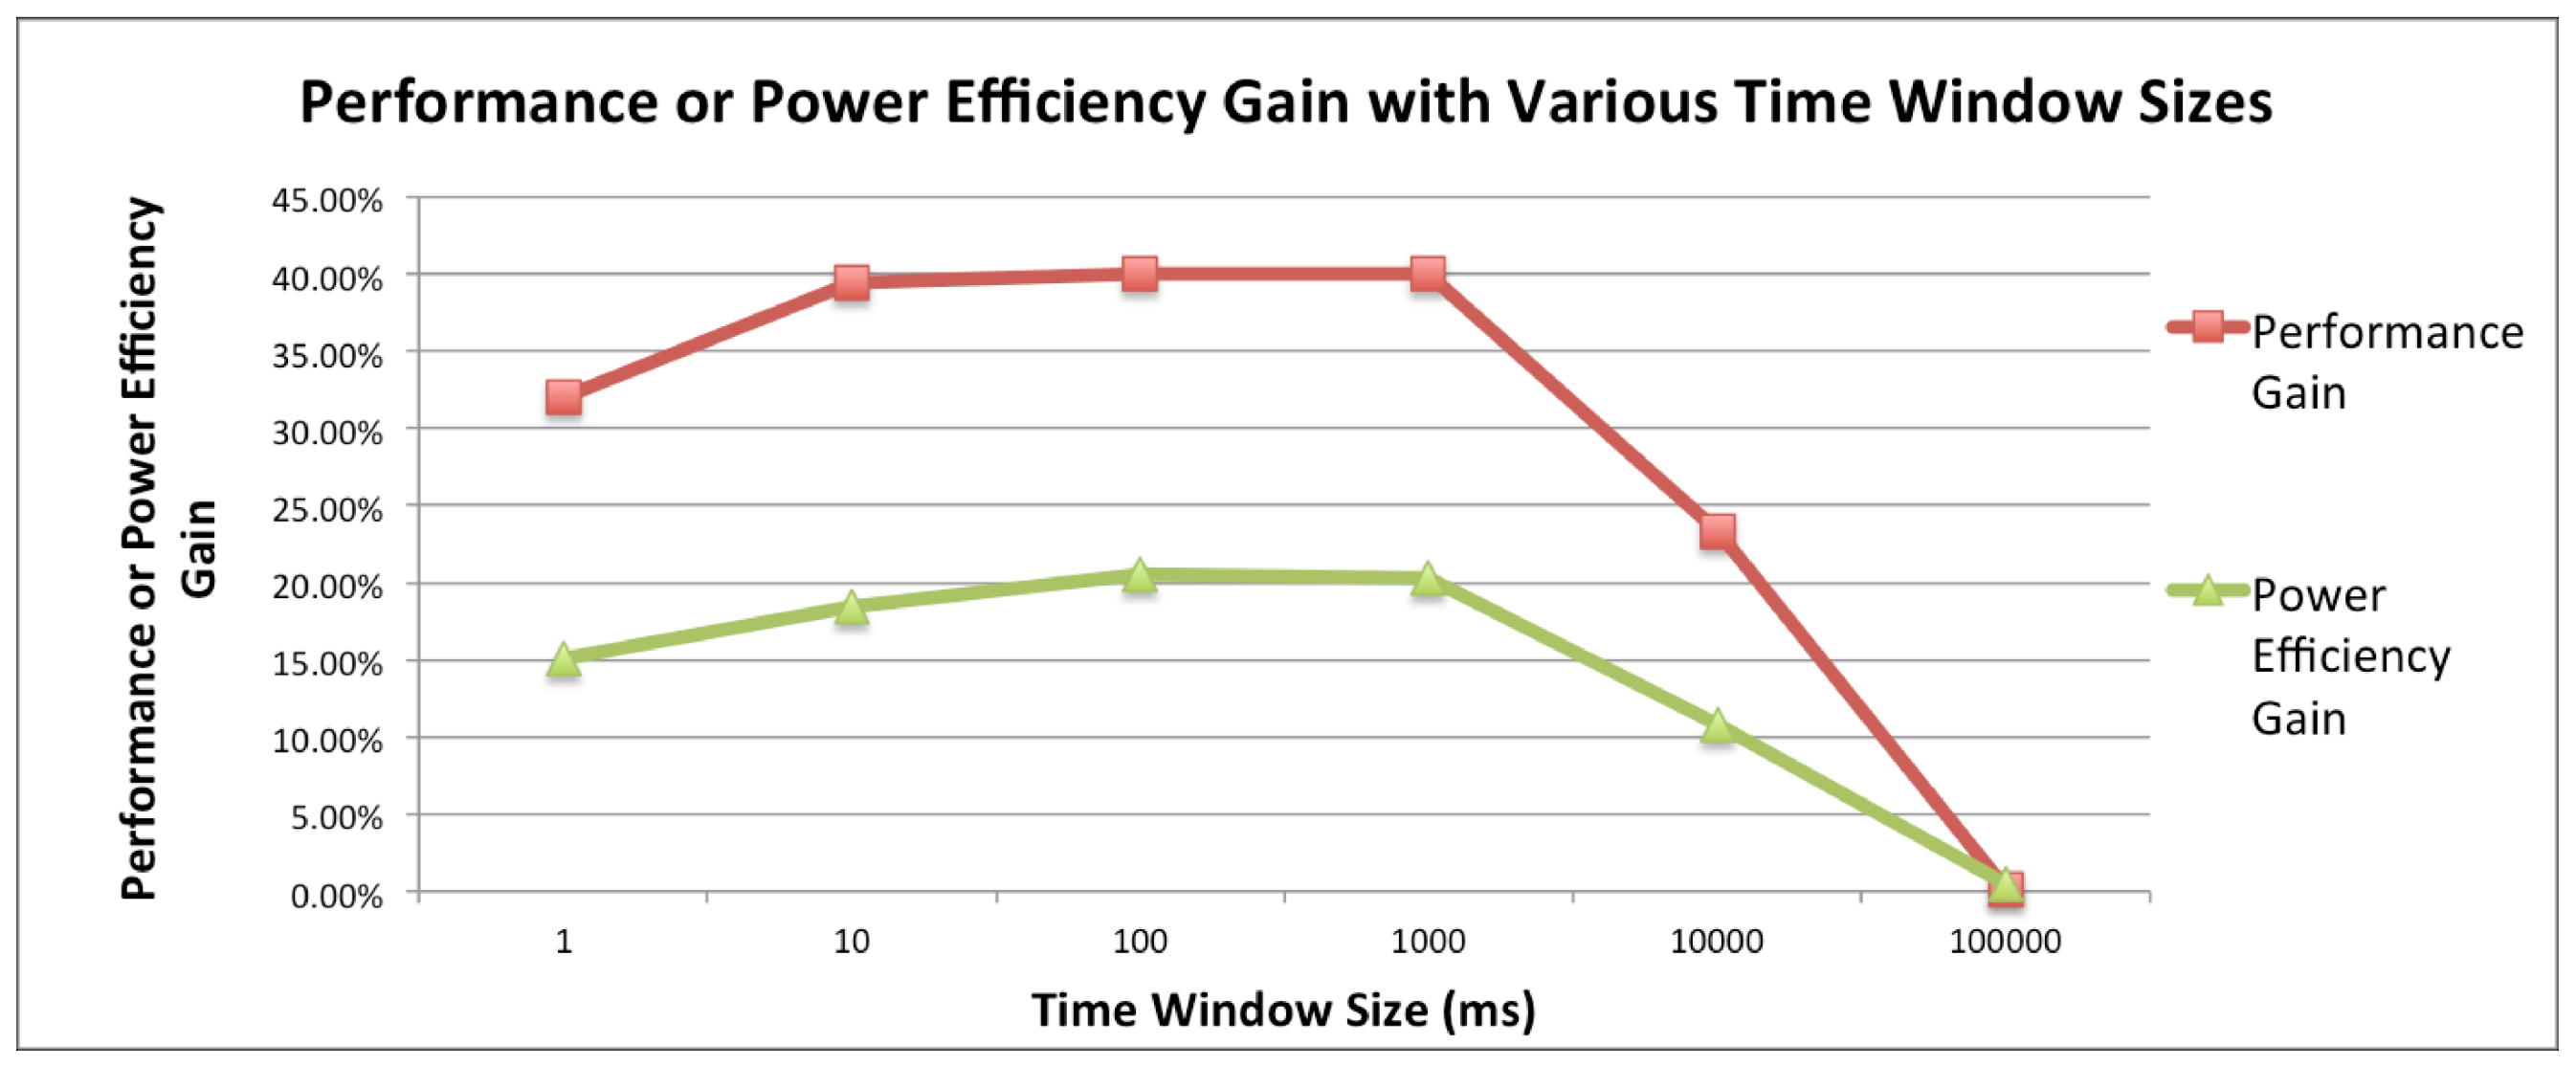
\includegraphics[width=4.5in]{Time-Window-Size}
    \caption{Performance and Power Analysis with Various Time Window Sizes}
    \label{fig_time_window}
\end{figure}

\subsubsection{Impact of Accelerator Scheduling on Memory-bound vs CPU-bound Applications}

We study the impact of the two scheduling heuristics, bandwidth-first
and speedup-first, for different types of workloads. Furthermore, we compare each of the
heuristics to na\"{\i}ve scheduling, in which case we simply use the calculated priority
rank $P_x$.  We construct two workload bundles based on the memory
access intensity for the benchmarks. The first workload bundle is memory-bound, with a bandwidth of over 500MB/s as shown in 
in Table \ref{tbl_benchmark}. The second workload bundle is CPU-bound.

By design, the
bandwidth-first strategy prioritizes the utilization of memory
bandwidth, which inherently gives benchmarks hungry for memory-bandwidth
more opportunities to take advantage of the accelerator logic. As a result,
this strategy outperforms speedup-first for memory-bound
applications as shown in Figure \ref{fig_mem_bound}. On the other hand,
CPU-bound applications benefit more from the speedup-first
scheduling strategy as depicted in Figure \ref{fig_cpu_bound}.

\begin{figure}
    \centering
    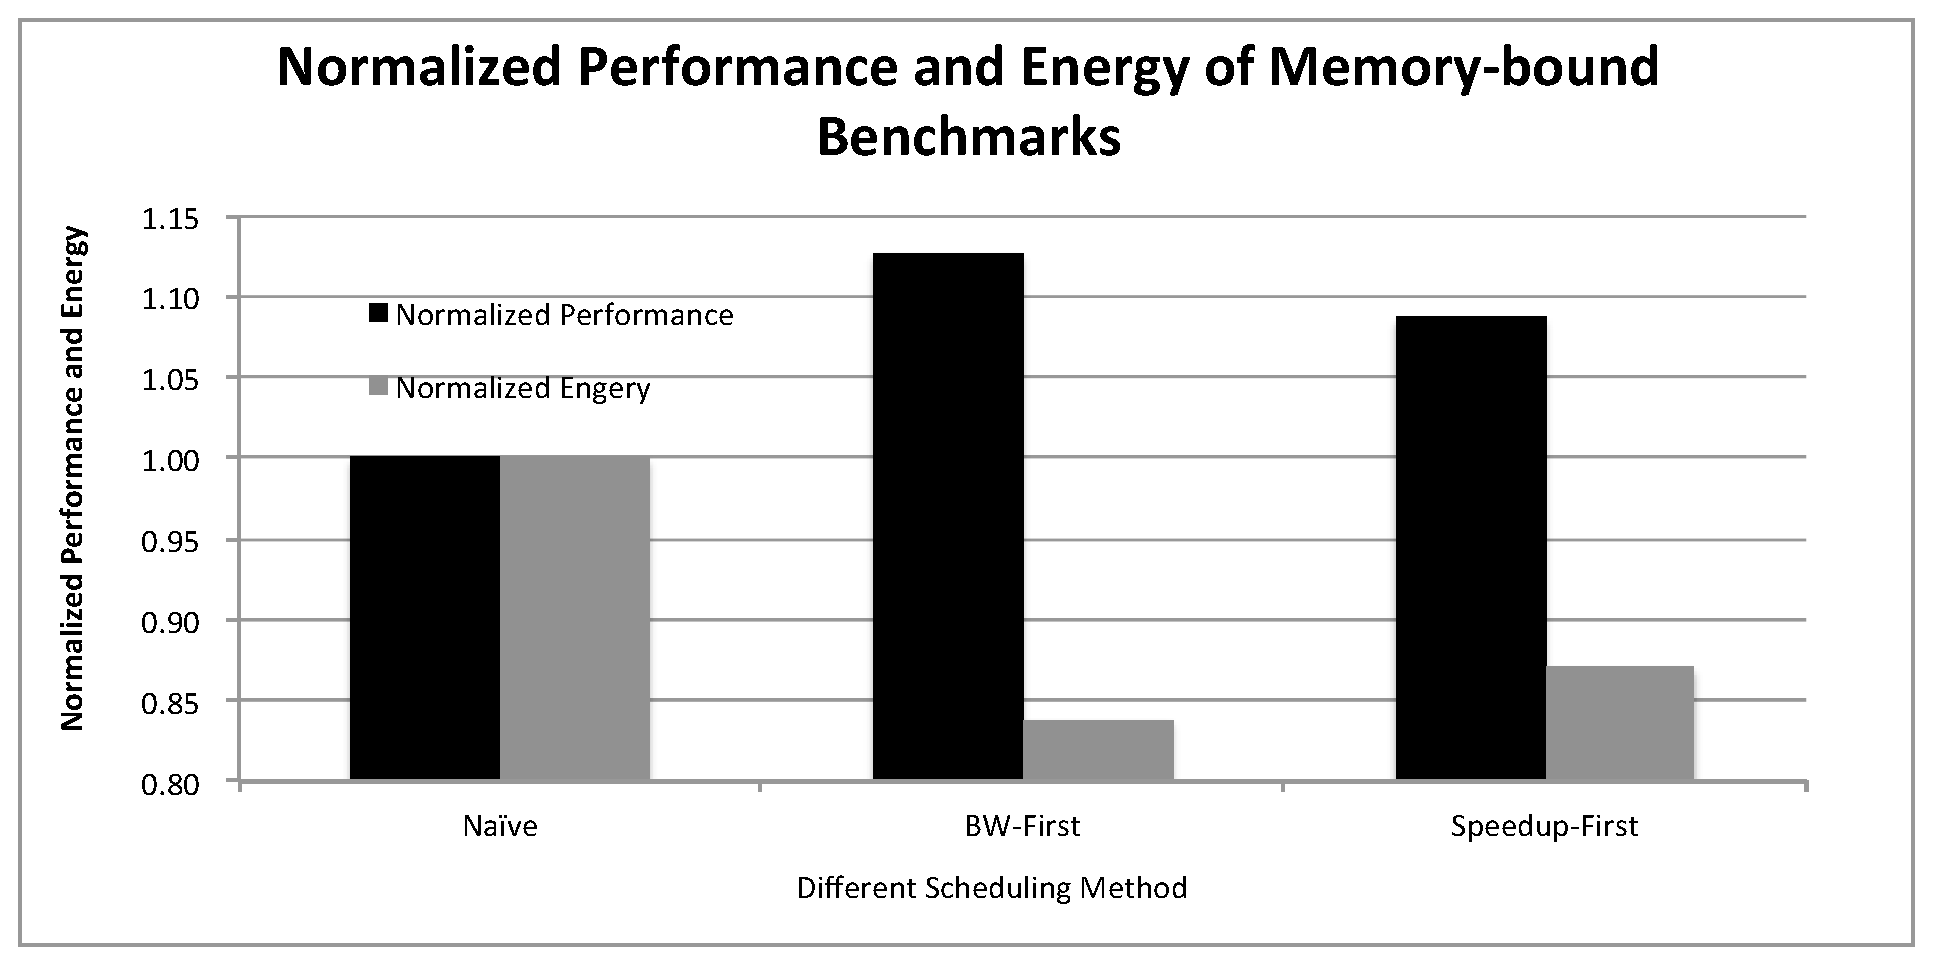
\includegraphics[width=4.5in]{Memory-Bounded}
    \caption{Performance and Energy Consumption of Memory-bound Benchmark Group}
    \label{fig_mem_bound}
\end{figure}

\begin{figure}
    \centering
    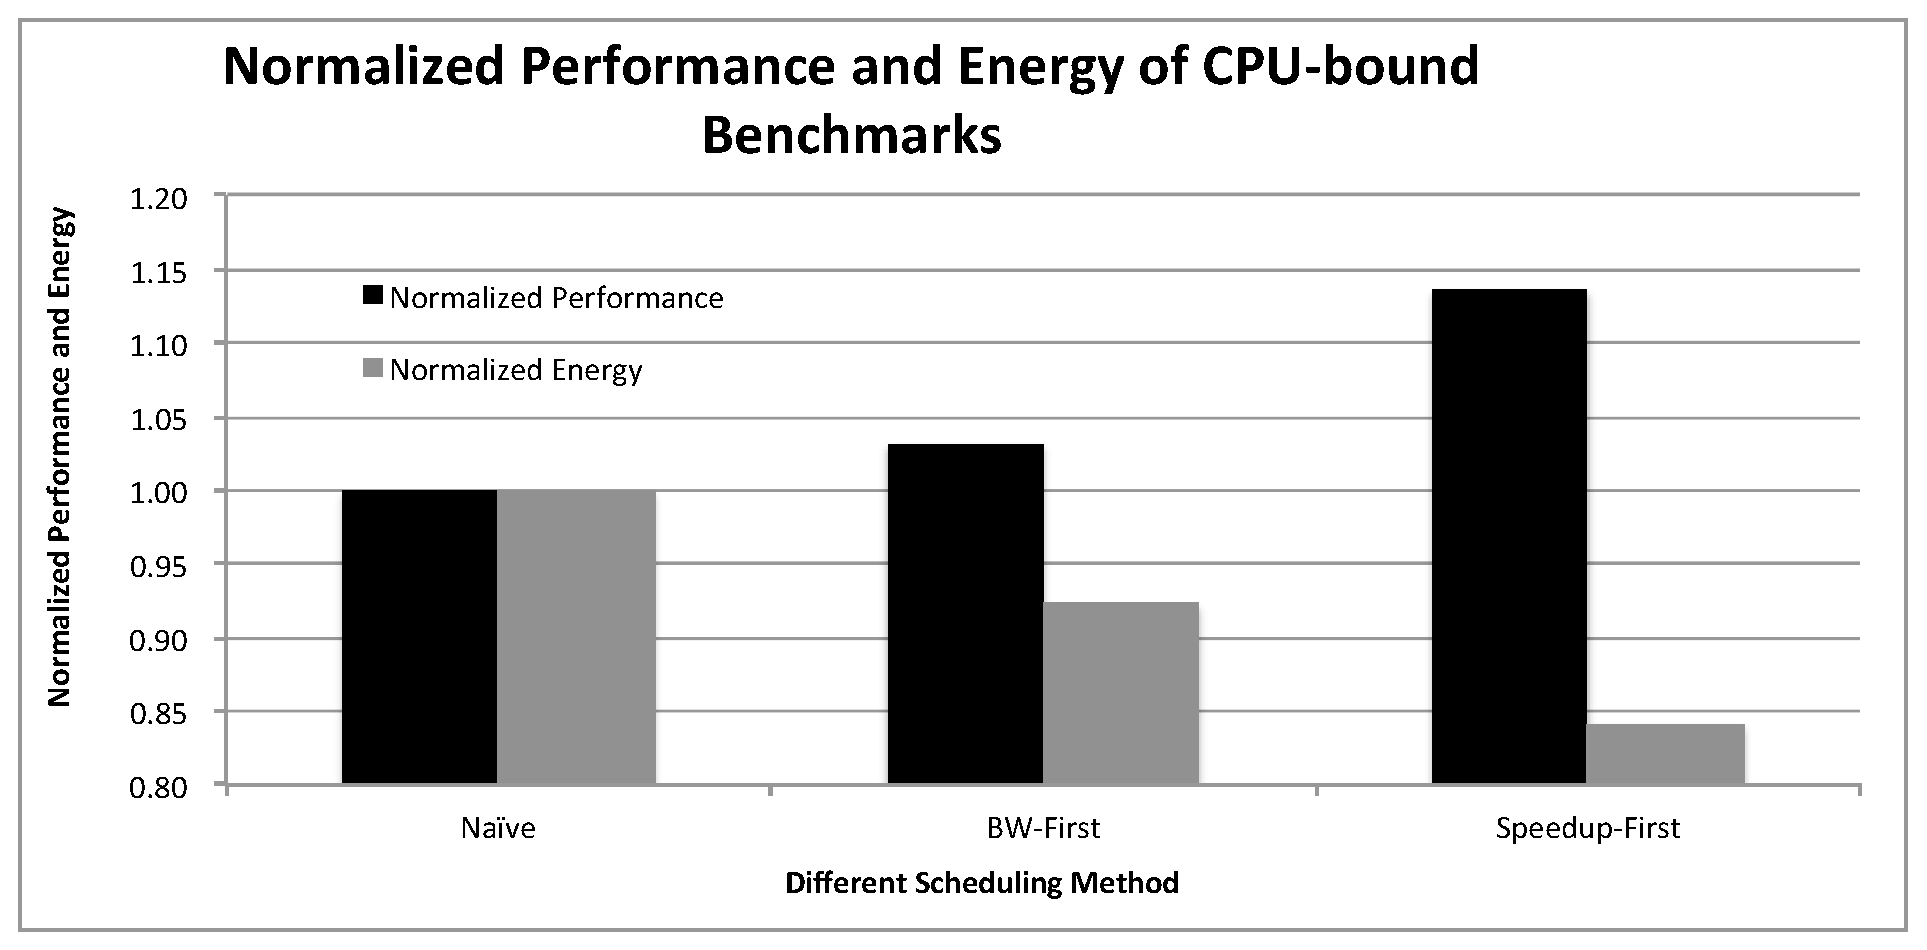
\includegraphics[width=4.5in]{CPU-Bounded}
    \caption{Performance and Energy Consumption on CPU-bound Benchmark Group}
    \label{fig_cpu_bound}
\end{figure}


\subsubsection{Chip Area Allocation}

Given the limited chip area, one particular area of interest is the method utilized for allocating space
 to each of the cores as well as the programmable accelerators.
We vary the number of cores and the size of the
reconfigurable logic to explore the design space. Figure
\ref{fig_core_acc_ratio} was obtained by changing the core and
the accelerator area ratio given a total area equivalent to four cores
as well as a reconfigurable logic unit, which in this case was a default accelerator size similar to the one used
by the Spartan 3E FPGA. As the area of an Atom core is about
    one fourth the size of a Spartan 3E FPGA, the resulting combinations for the cores and the reconfigurable
logic include 8:0, 6:0.5, and so forth. It is interesting to note that the
 5:0.75 ratio produces optimal performance gains while increasing the accelerator
logic continually improves the energy efficiency. While the ratios are
specific to each of the workloads and therefore can only be generalized with caution, 
our results indicate that it is important to
investigate the design space in order to determine the best possible
arrangement for the cores as well as the accelerators. 

\begin{figure}
    \centering
    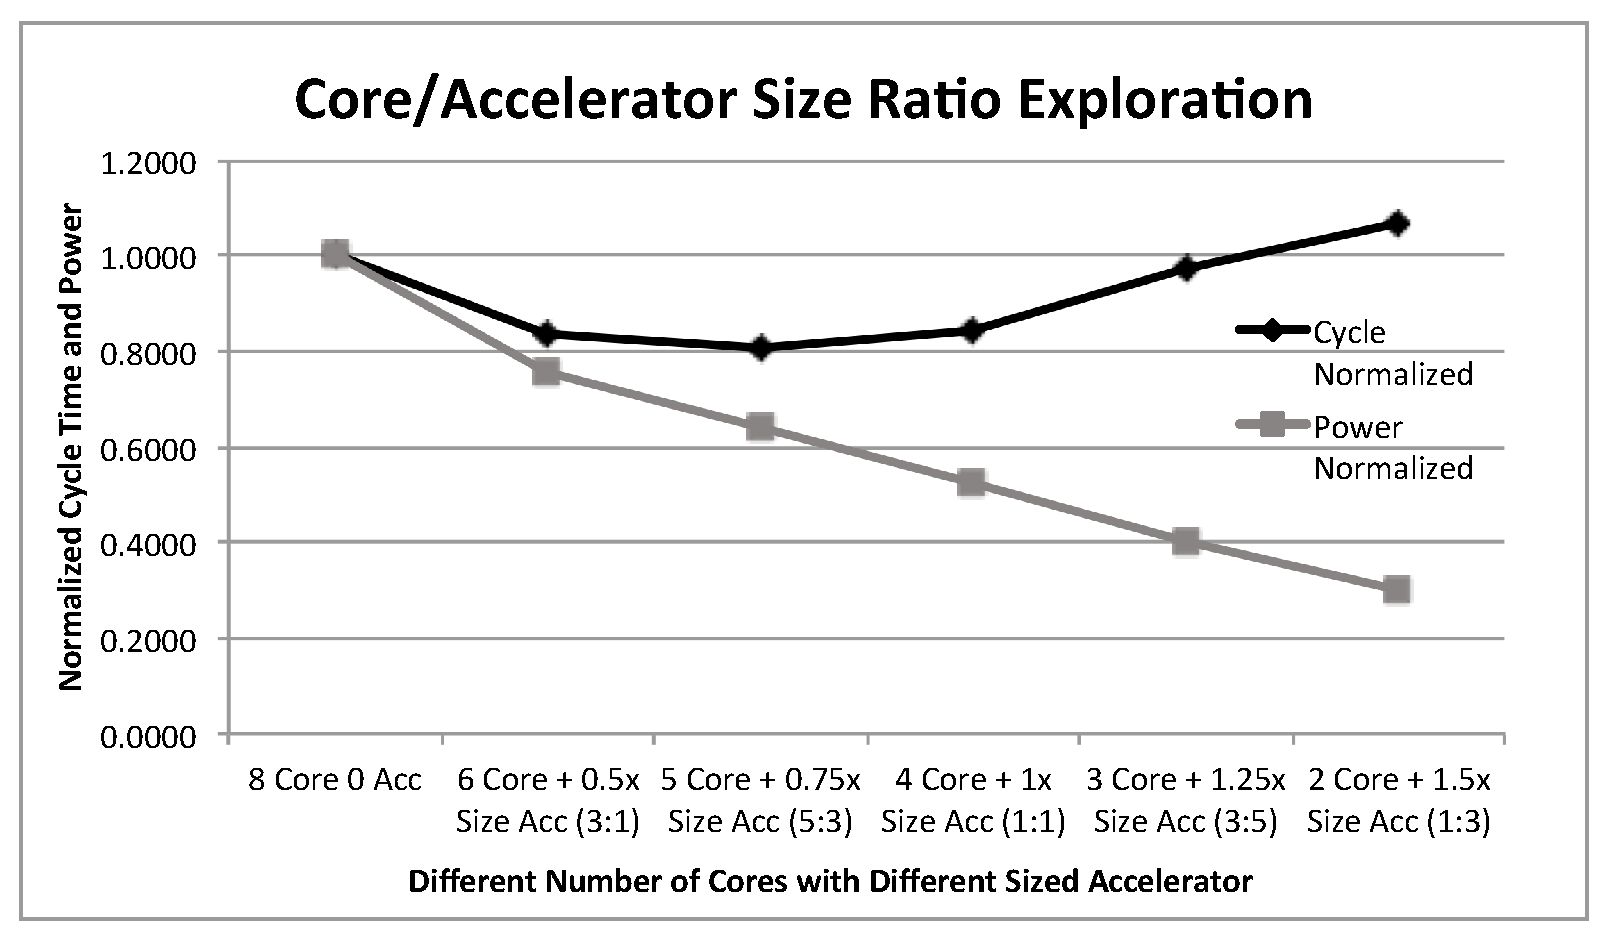
\includegraphics[width=4.5in]{Core-Acc-Size-Ratio}
    \caption{Performance and Power with Different Core/Accelerator Ratios}
    \label{fig_core_acc_ratio}
\end{figure}

\subsubsection{Architectural Parameter Analysis}

One of the contributions of this work is to provide insights into how
different parameters of the heterogeneous architecture or the
benchmark will affect the performance and the power efficiency of the
resulting heterogeneous architecture. Thus, we explore the same performance and
energy efficiency metrics with respect to different architectural parameters in order to
 better understand their implications. 

First, we study the effects of the L1 cache size as shown in Figure \ref{fig_l1_perf}. Our
system consisting of 32 KB of L1 cache employing a na\"{\i}ve scheduling algorithm is considered as the
baseline for this experiment. The performance gain increases rapidly as the
L1 cache size changes from 8 KB to 32 KB, specifically between 12\% to 14\%.
However, the performance gains decrease as the cache size increases beyond 32
KB. The aforementioned findings indicate that 32 KB of L1 cache is sufficiently large
 for our benchmarks. As shown in Figure
\ref{fig_l1_power}, the power efficiency decreases
steadily as the cache size increases. In this case, the increase in the cache size 
tends to significantly increase both the static power as well as the dynamic power. 

We conduct a similar experiment by changing the L2 cache size, displaying
the results in Figure \ref{fig_l2_perf} and \ref{fig_l2_power}. As
we increase the size of the L2 cache, the performance gain increases while the
power efficiency gain steadily decreases. However, the slope of the gain is significantly larger by comparison with the results obtained for 
the L1 cache. In this case, the accelerators and the CPUs share the L2 cache with the MOESI coherence. As a result, when the cache size 
increases, the heterogeneous architecture benefits from the lower cache miss rate. 

The accelerator's local buffer works in similar manner to the core's L1 cache. Thus, the characteristics of the accelerator local buffer 
resemble the characteristics of the L1 cache as shown in Figure \ref{fig_acc_buffer_perf} and \ref{fig_acc_buffer_power}. 
The only difference is that as we adjust the buffer size, the rate of change for the gains of the local buffer is larger 
by comparison with the L1 cache. In this case the hardware implementation is more sensitive to the locality of the input data
 given that there is a higher level of data parallelism within the accelerators. 

We also study the inter-arrival time of the Poisson-distributed benchmark mixture to find if the dynamics of the workload will affect 
system performance. As illustrated in Figure \ref{fig_benchmark-switching}, we take the 500 million cycles inter-arrival time with na\"{\i}ve
 scheduling as the baseline since ``500 million cycles" is the setup in our experiment. The performance gain tends to decrease as 
the benchmark inter-arrival time varies from 0 cycles to 1000 million cycles. When the inter-arrival time is set to 0 cycles, it becomes
 identical to the continuously arriving back-to-back workload. This figure demonstrates that the more frequent the change in the workload of 
the benchmarks, the more precise the profiling-prediction, and the larger the gains from the scheduling methods. The aforementioned gains
are realized in spite of the increasing overhead due to accelerator reprogramming. In addition, as the inter-arrival time increases, 
the difference in the performance gains increases when comparing the na\"{\i}ve scheduling methods with the other two methods. 
In this case, the benefits of prediction decrease as the inter-arrival time becomes significantly large. However, both the bandwidth-first and
 the speedup-first scheduling algorithms benefit from accelerator combination. 

\begin{figure}
    \centering
    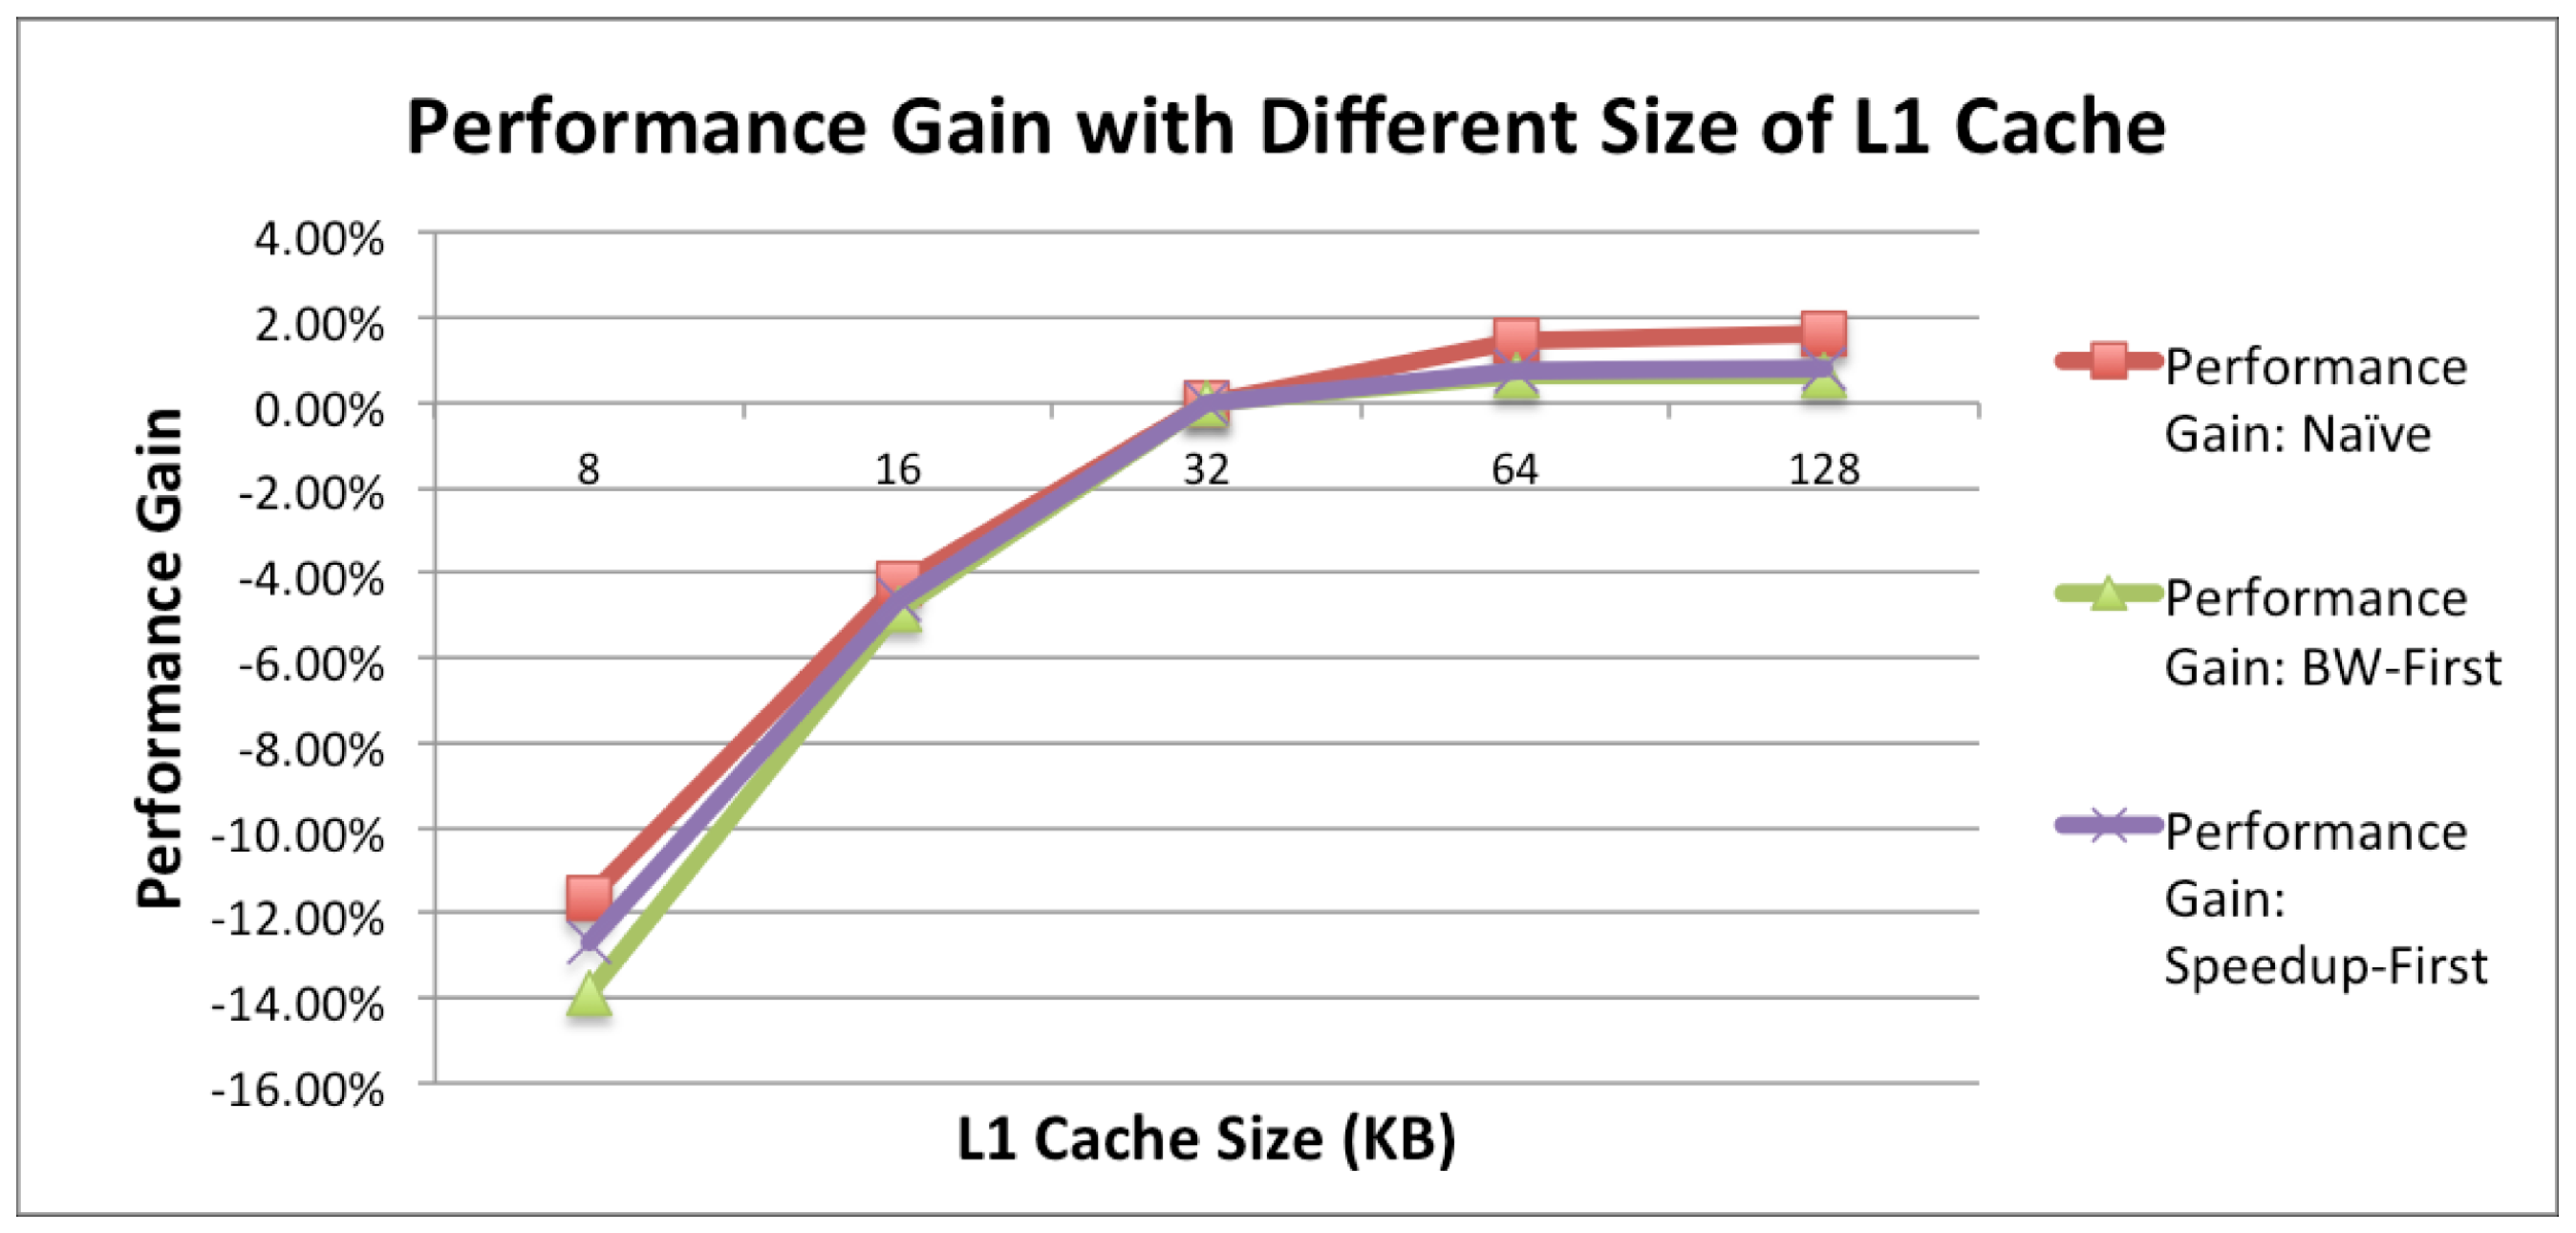
\includegraphics[width=4.5in]{L1-Cache-Performance}
    \caption{Performance Gain with Different Sizes of L1 Cache}
    \label{fig_l1_perf}
\end{figure}

\begin{figure}
    \centering
    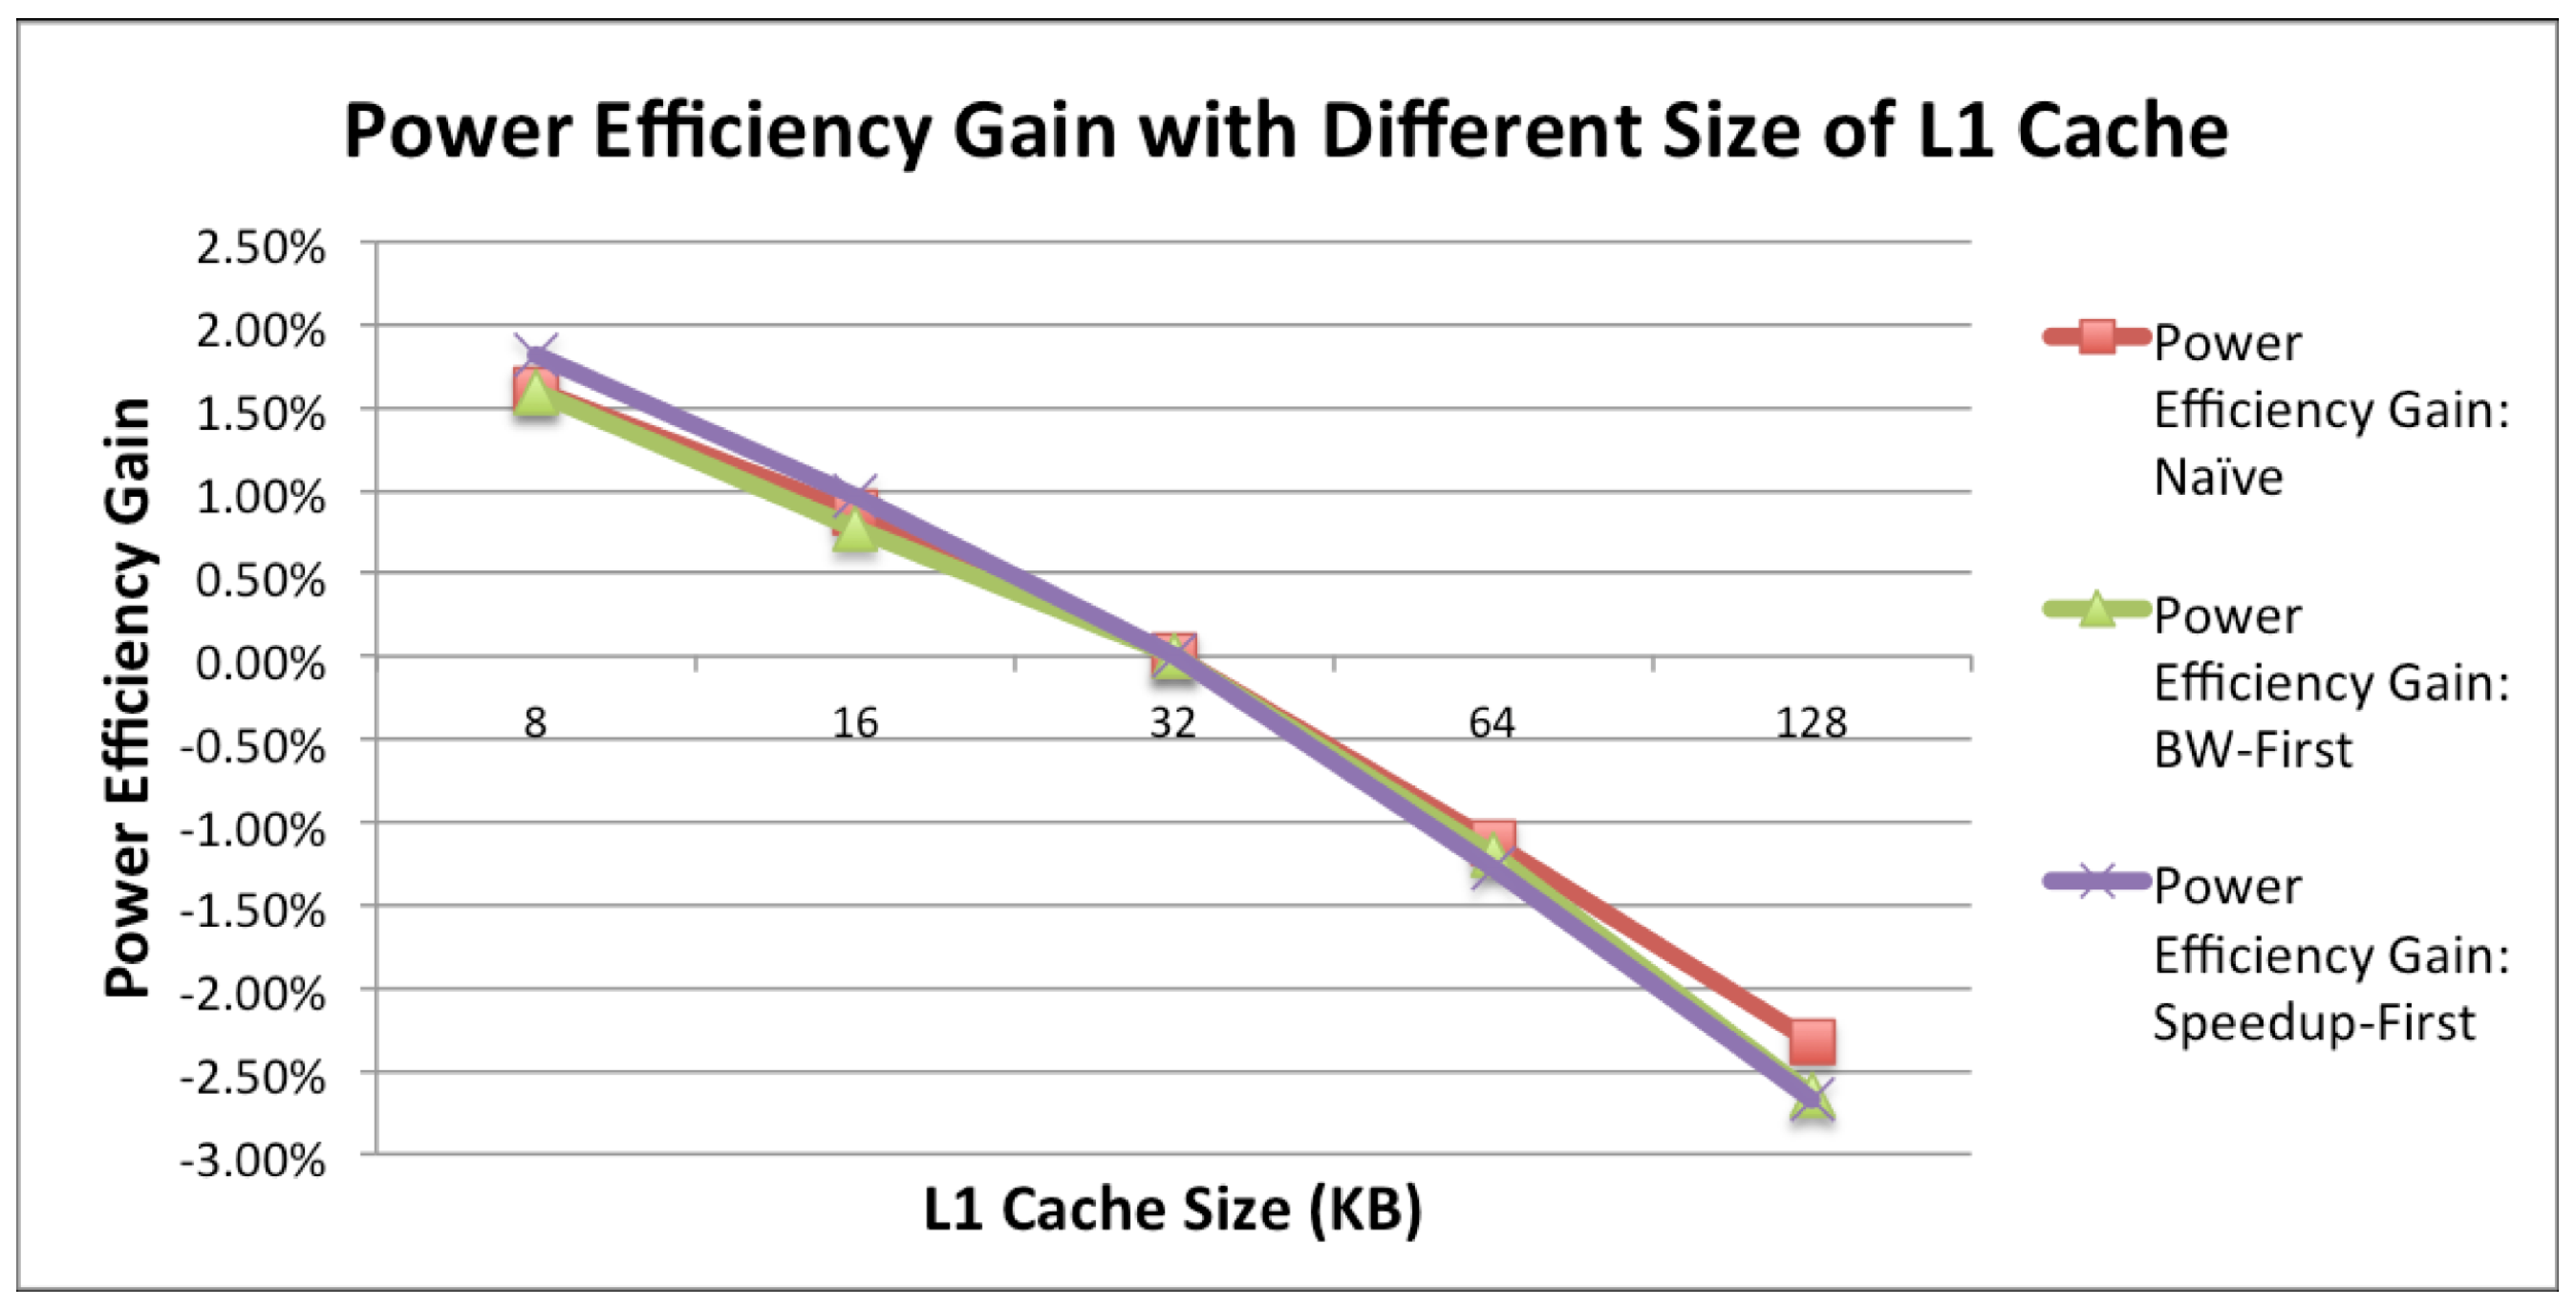
\includegraphics[width=4.5in]{L1-Cache-Power}
    \caption{Power Efficiency Gain with Different Sizes of L1 Cache}
    \label{fig_l1_power}
\end{figure}

\begin{figure}
    \centering
    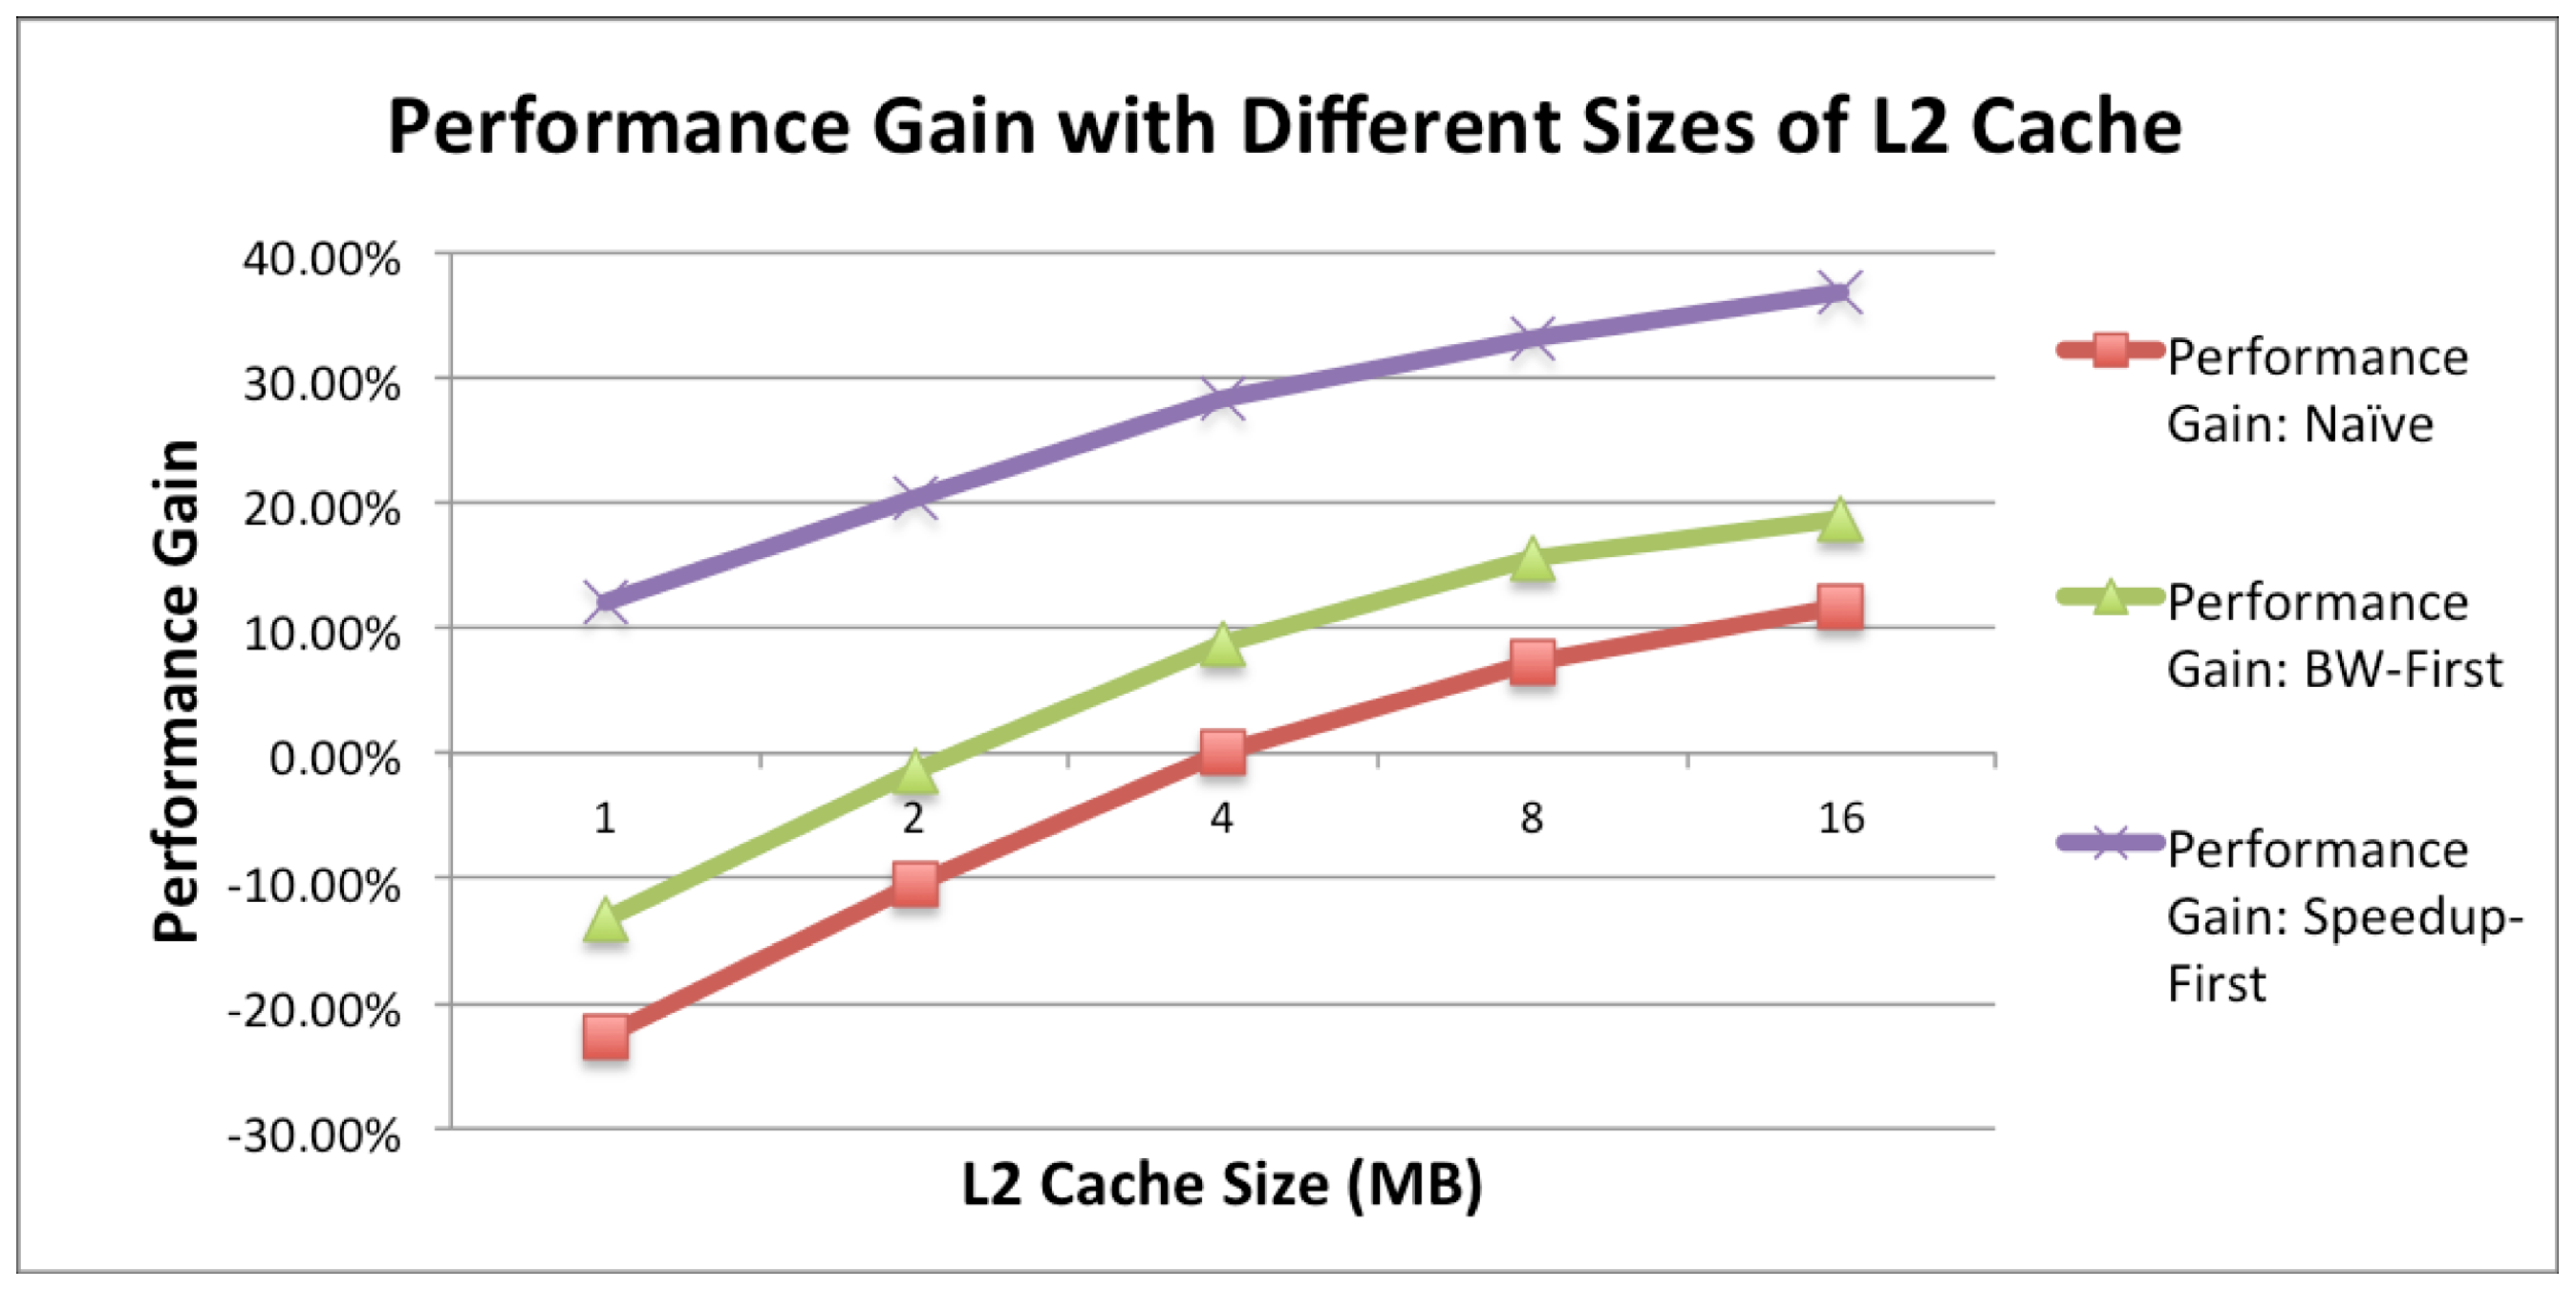
\includegraphics[width=4.5in]{L2-Cache-Performance}
    \caption{Performance Gain with Different Sizes of L2 Cache}
    \label{fig_l2_perf}
\end{figure}

\begin{figure}
    \centering
    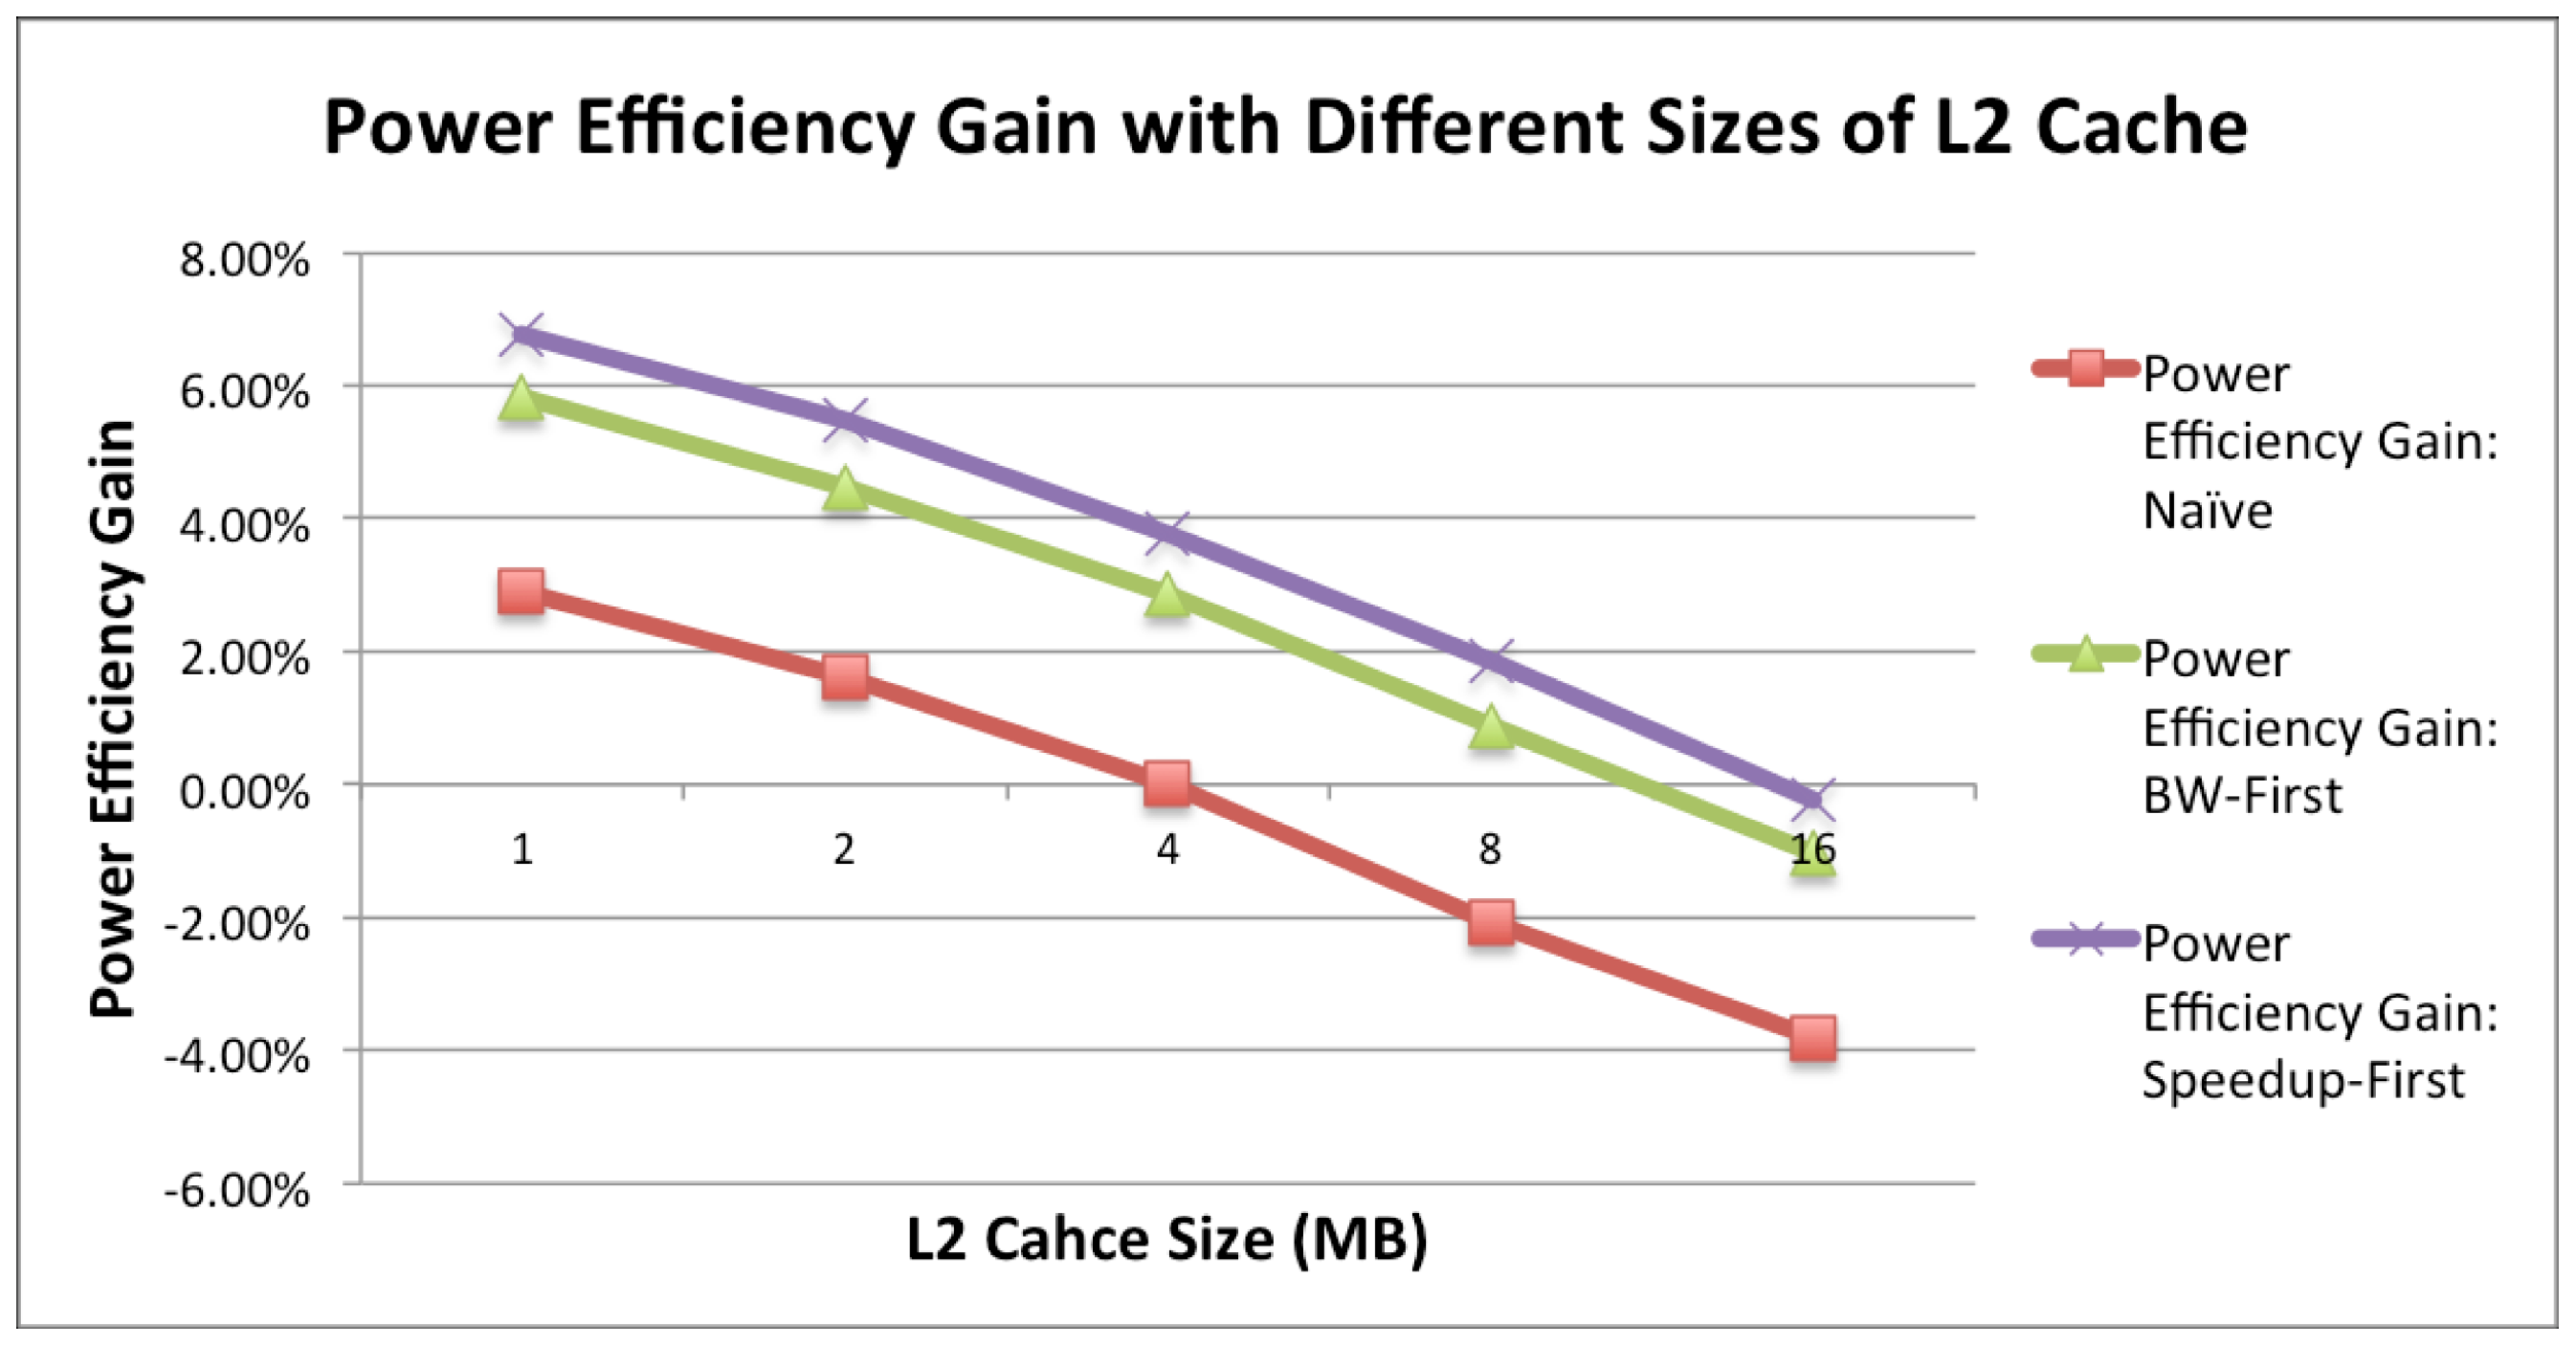
\includegraphics[width=4.5in]{L2-Cache-Power}
    \caption{Power Efficiency Gain with Different Sizes of L2 Cache}
    \label{fig_l2_power}
\end{figure}

\begin{figure}
    \centering
    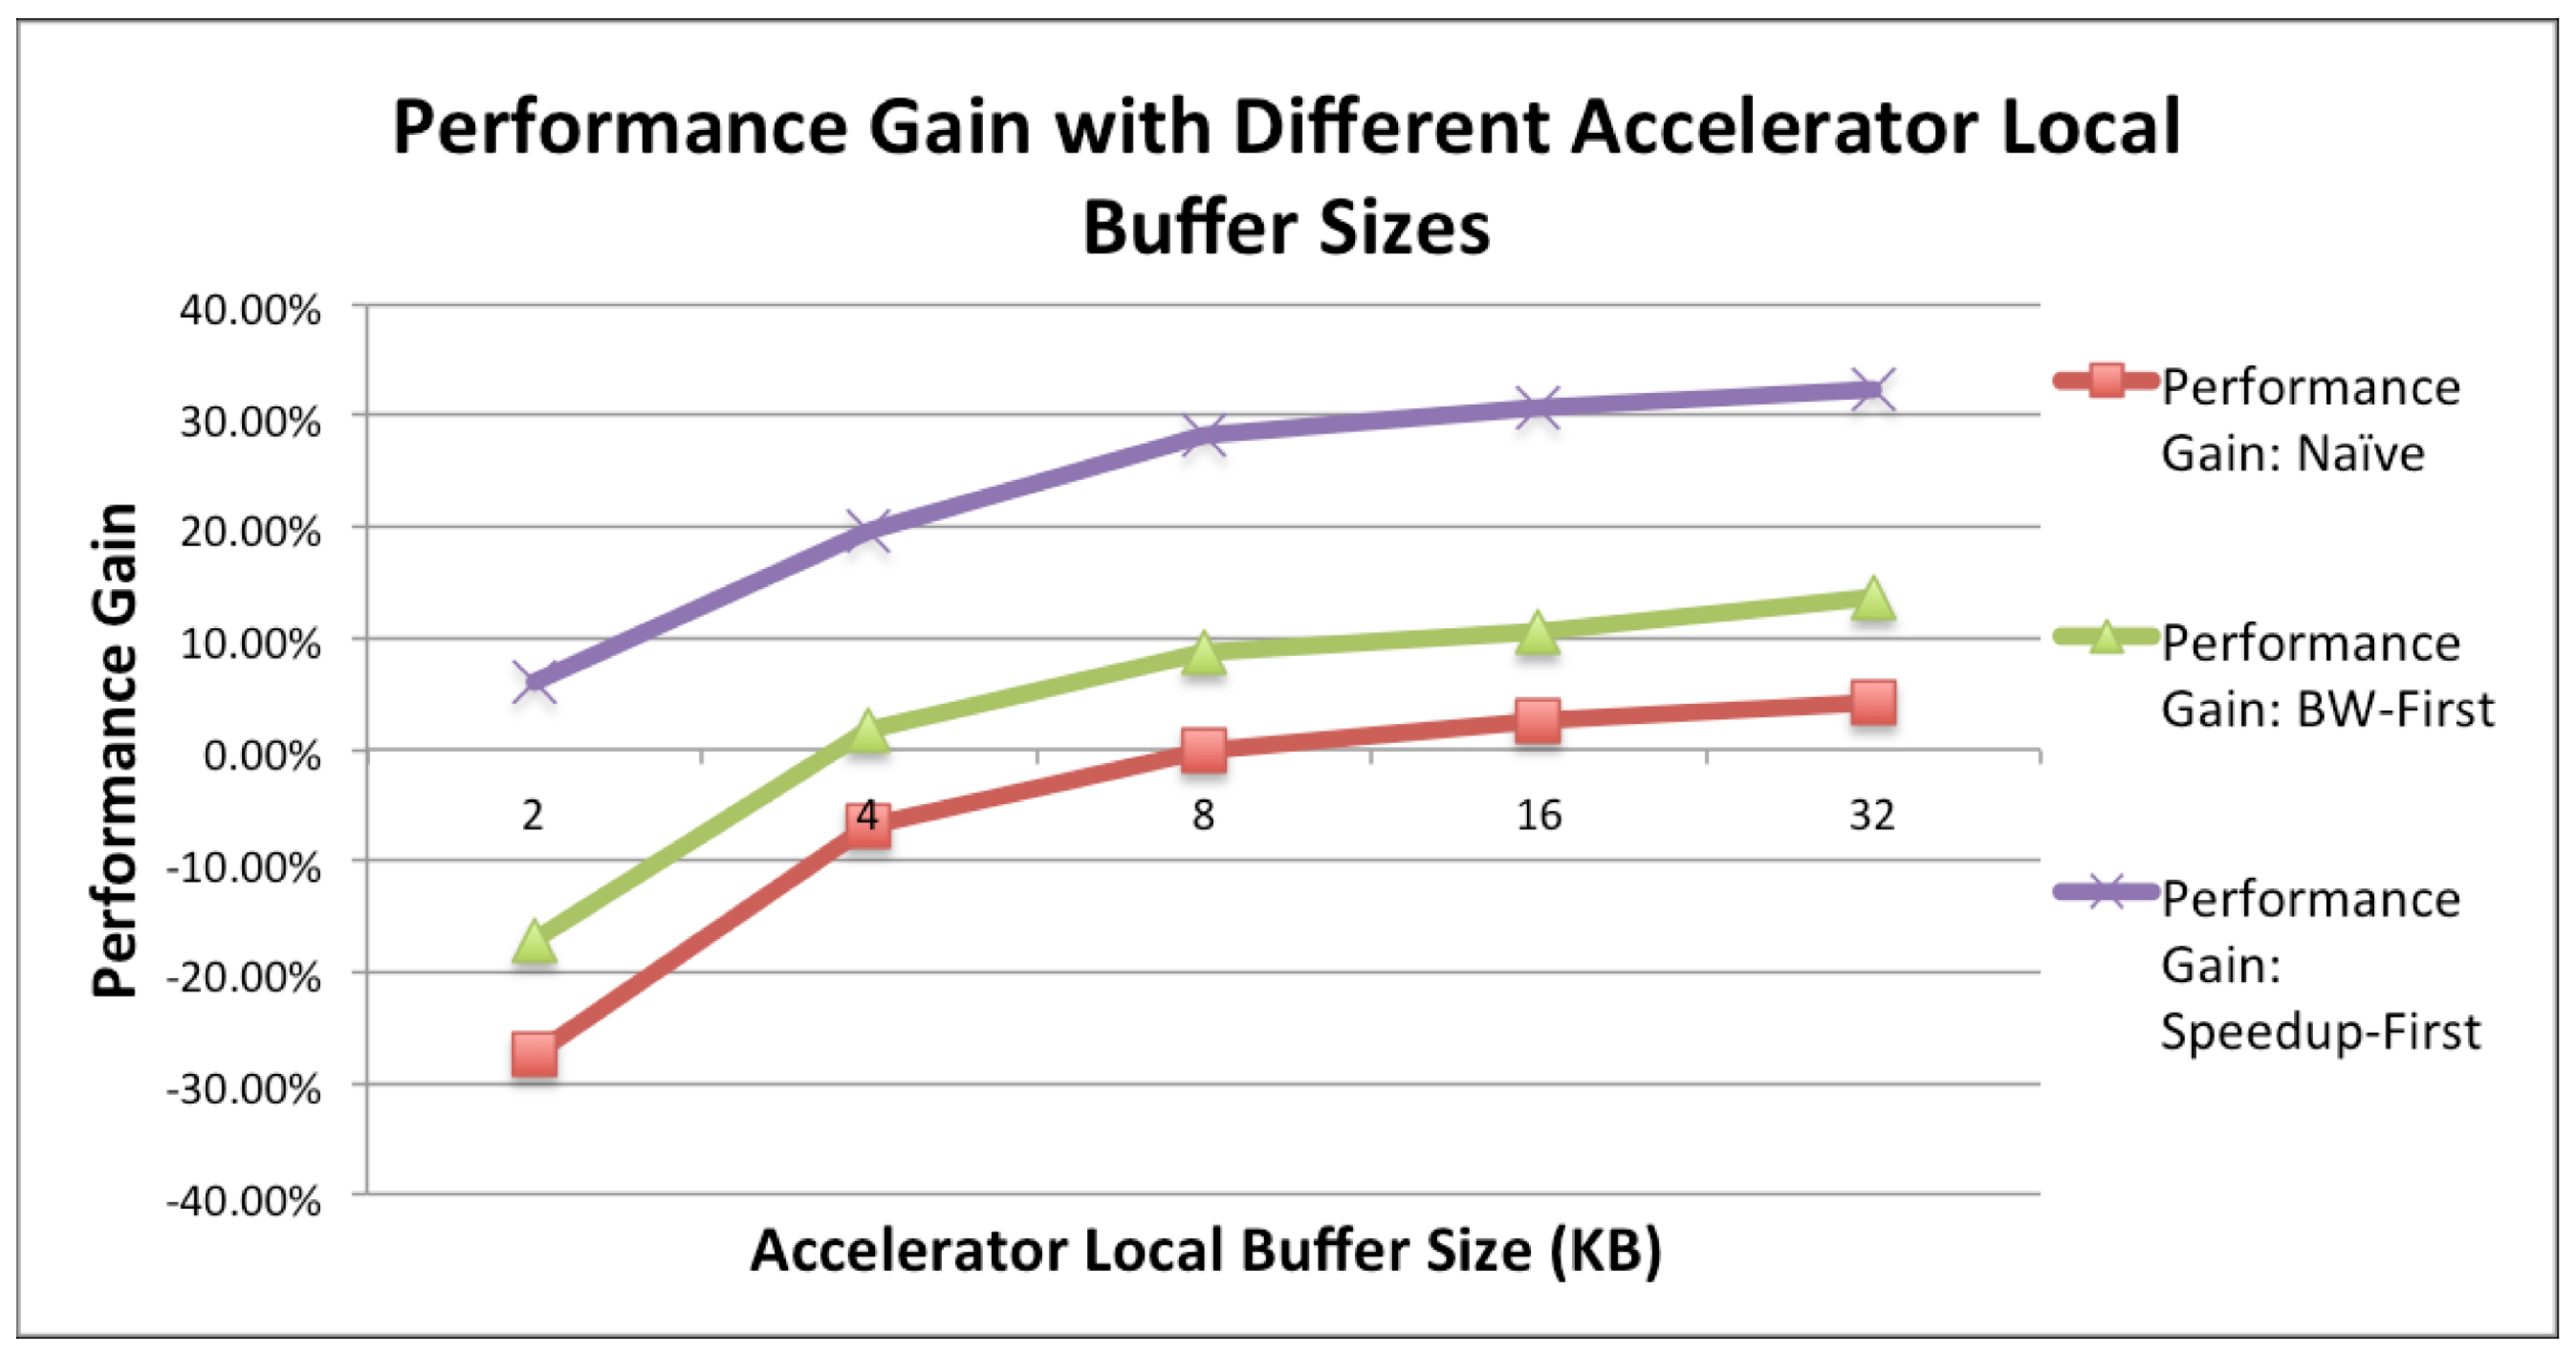
\includegraphics[width=4.5in]{Acc-Buffer-Performance}
    \caption{Performance Gain with Different Sizes of Accelerator Local Buffer}
    \label{fig_acc_buffer_perf}
\end{figure}

\begin{figure}
    \centering
    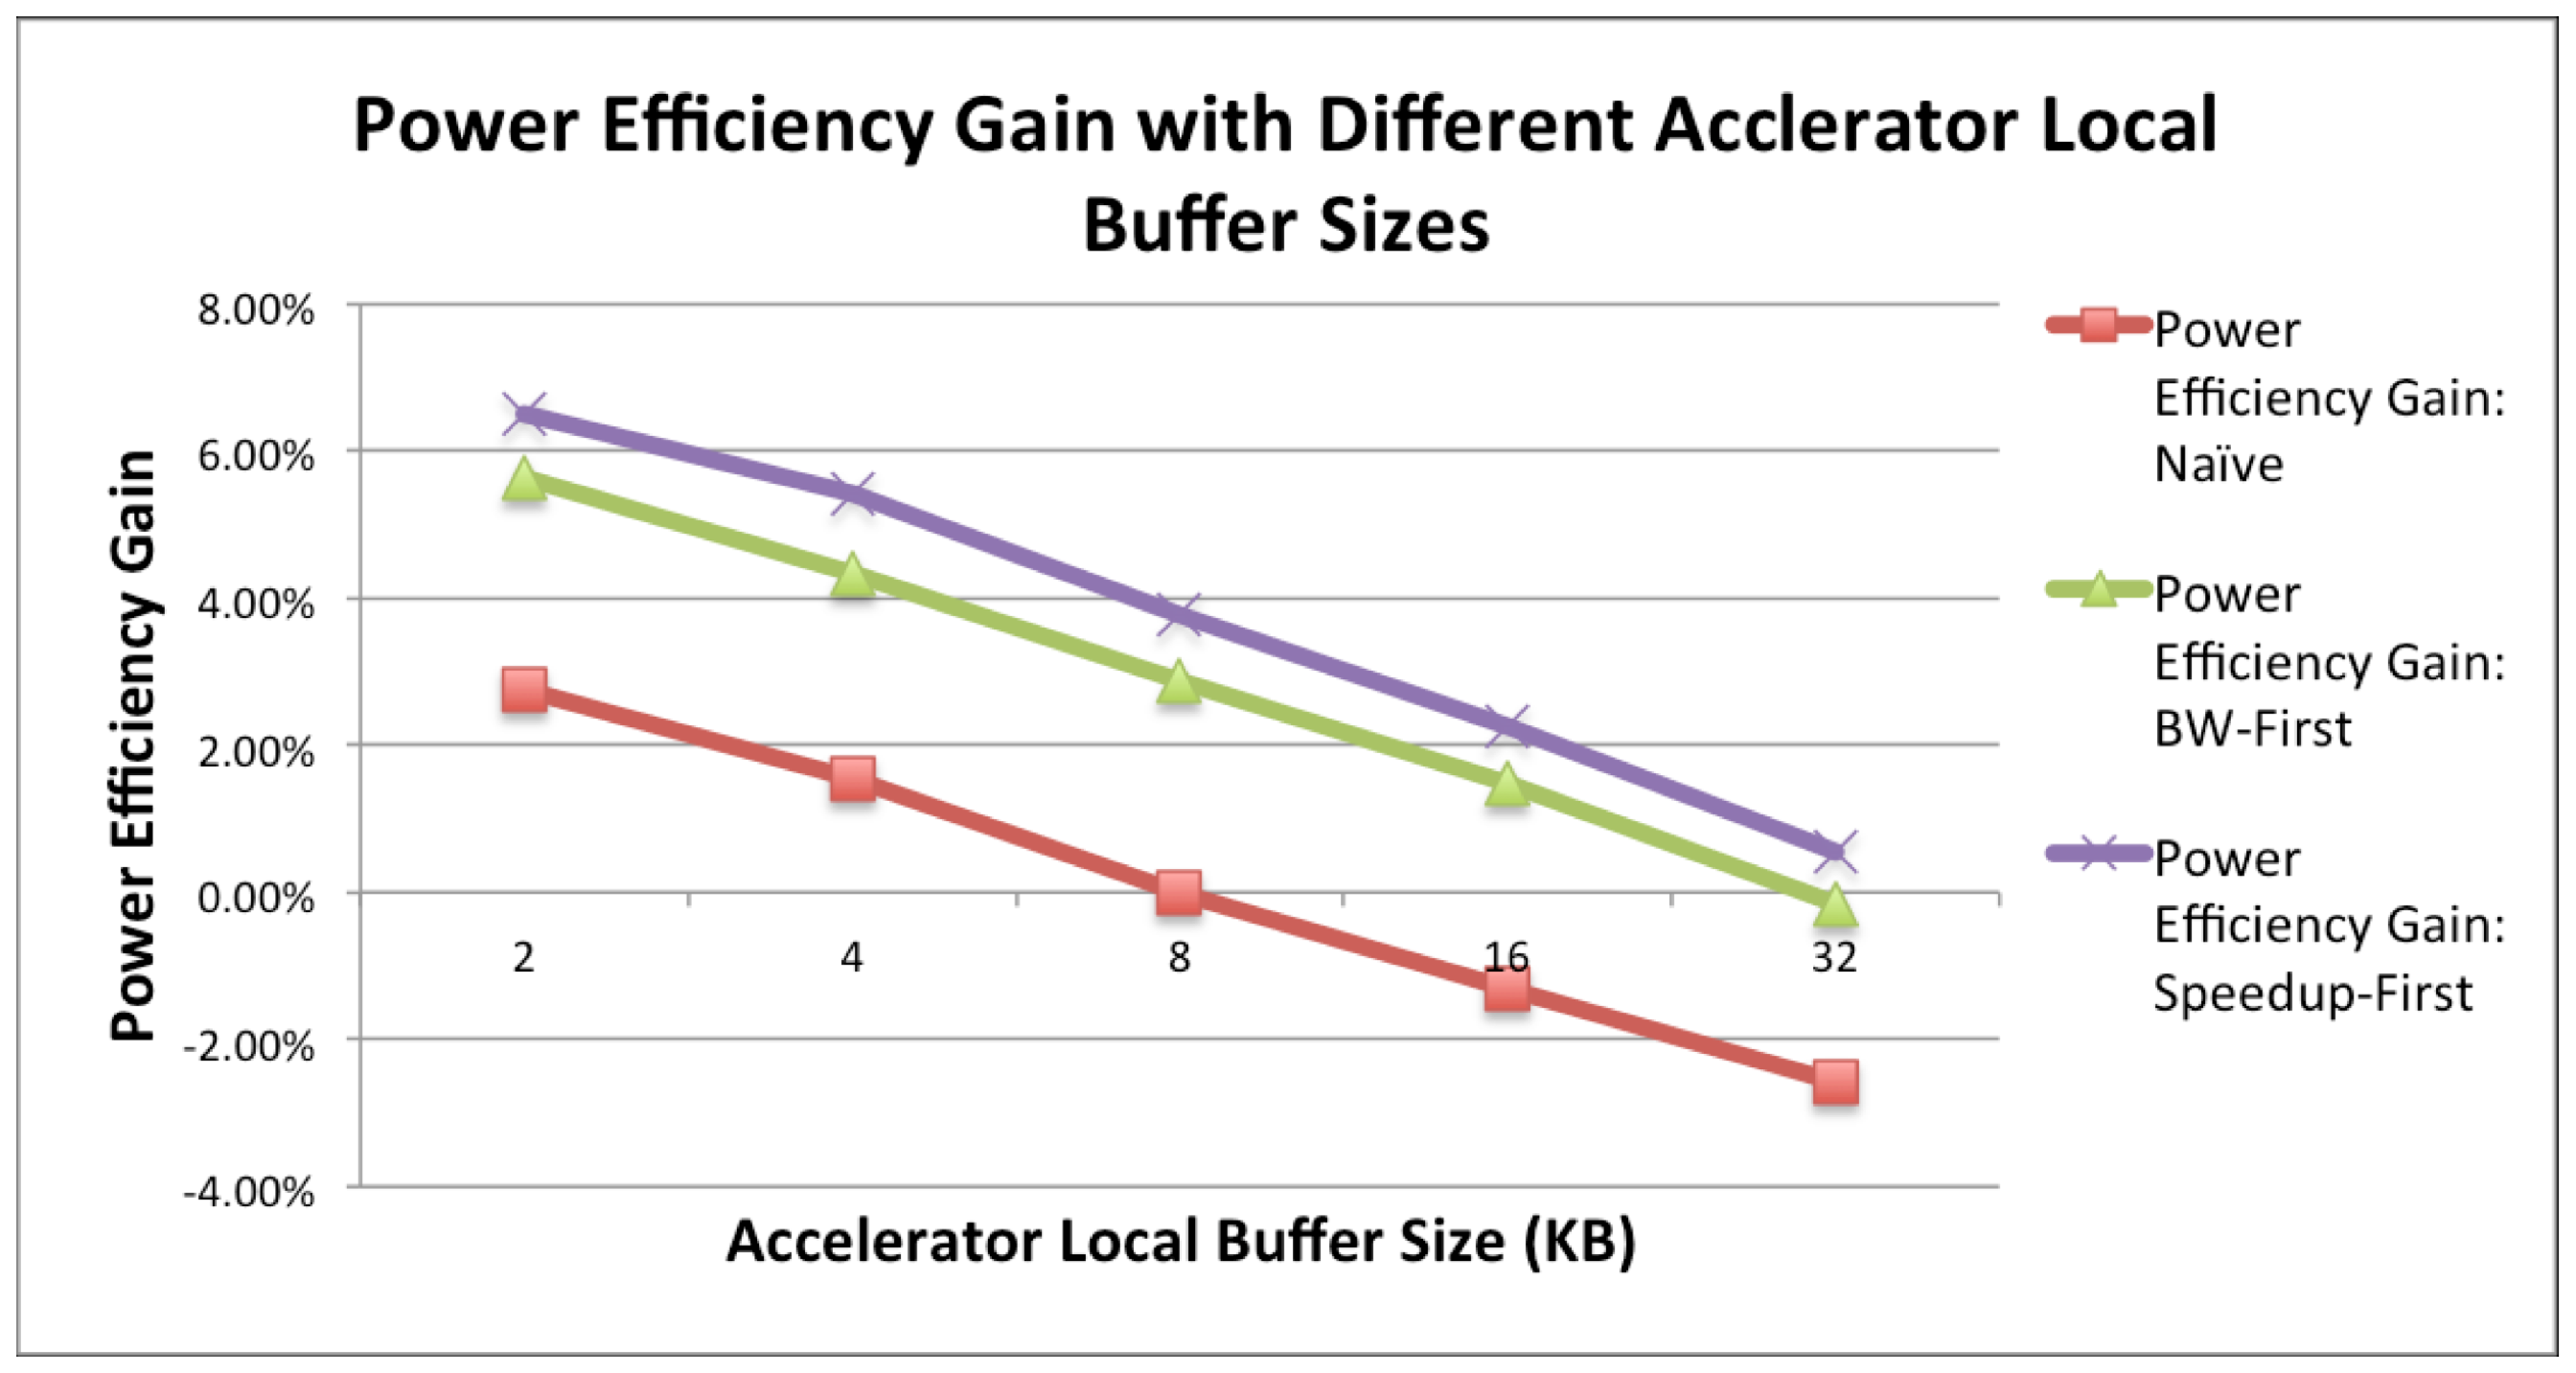
\includegraphics[width=4.5in]{Acc-Buffer-Power}
    \caption{Power Efficiency Gain with Different Sizes of Accelerator Local Buffer}
    \label{fig_acc_buffer_power}
\end{figure}

\begin{figure}
    \centering
    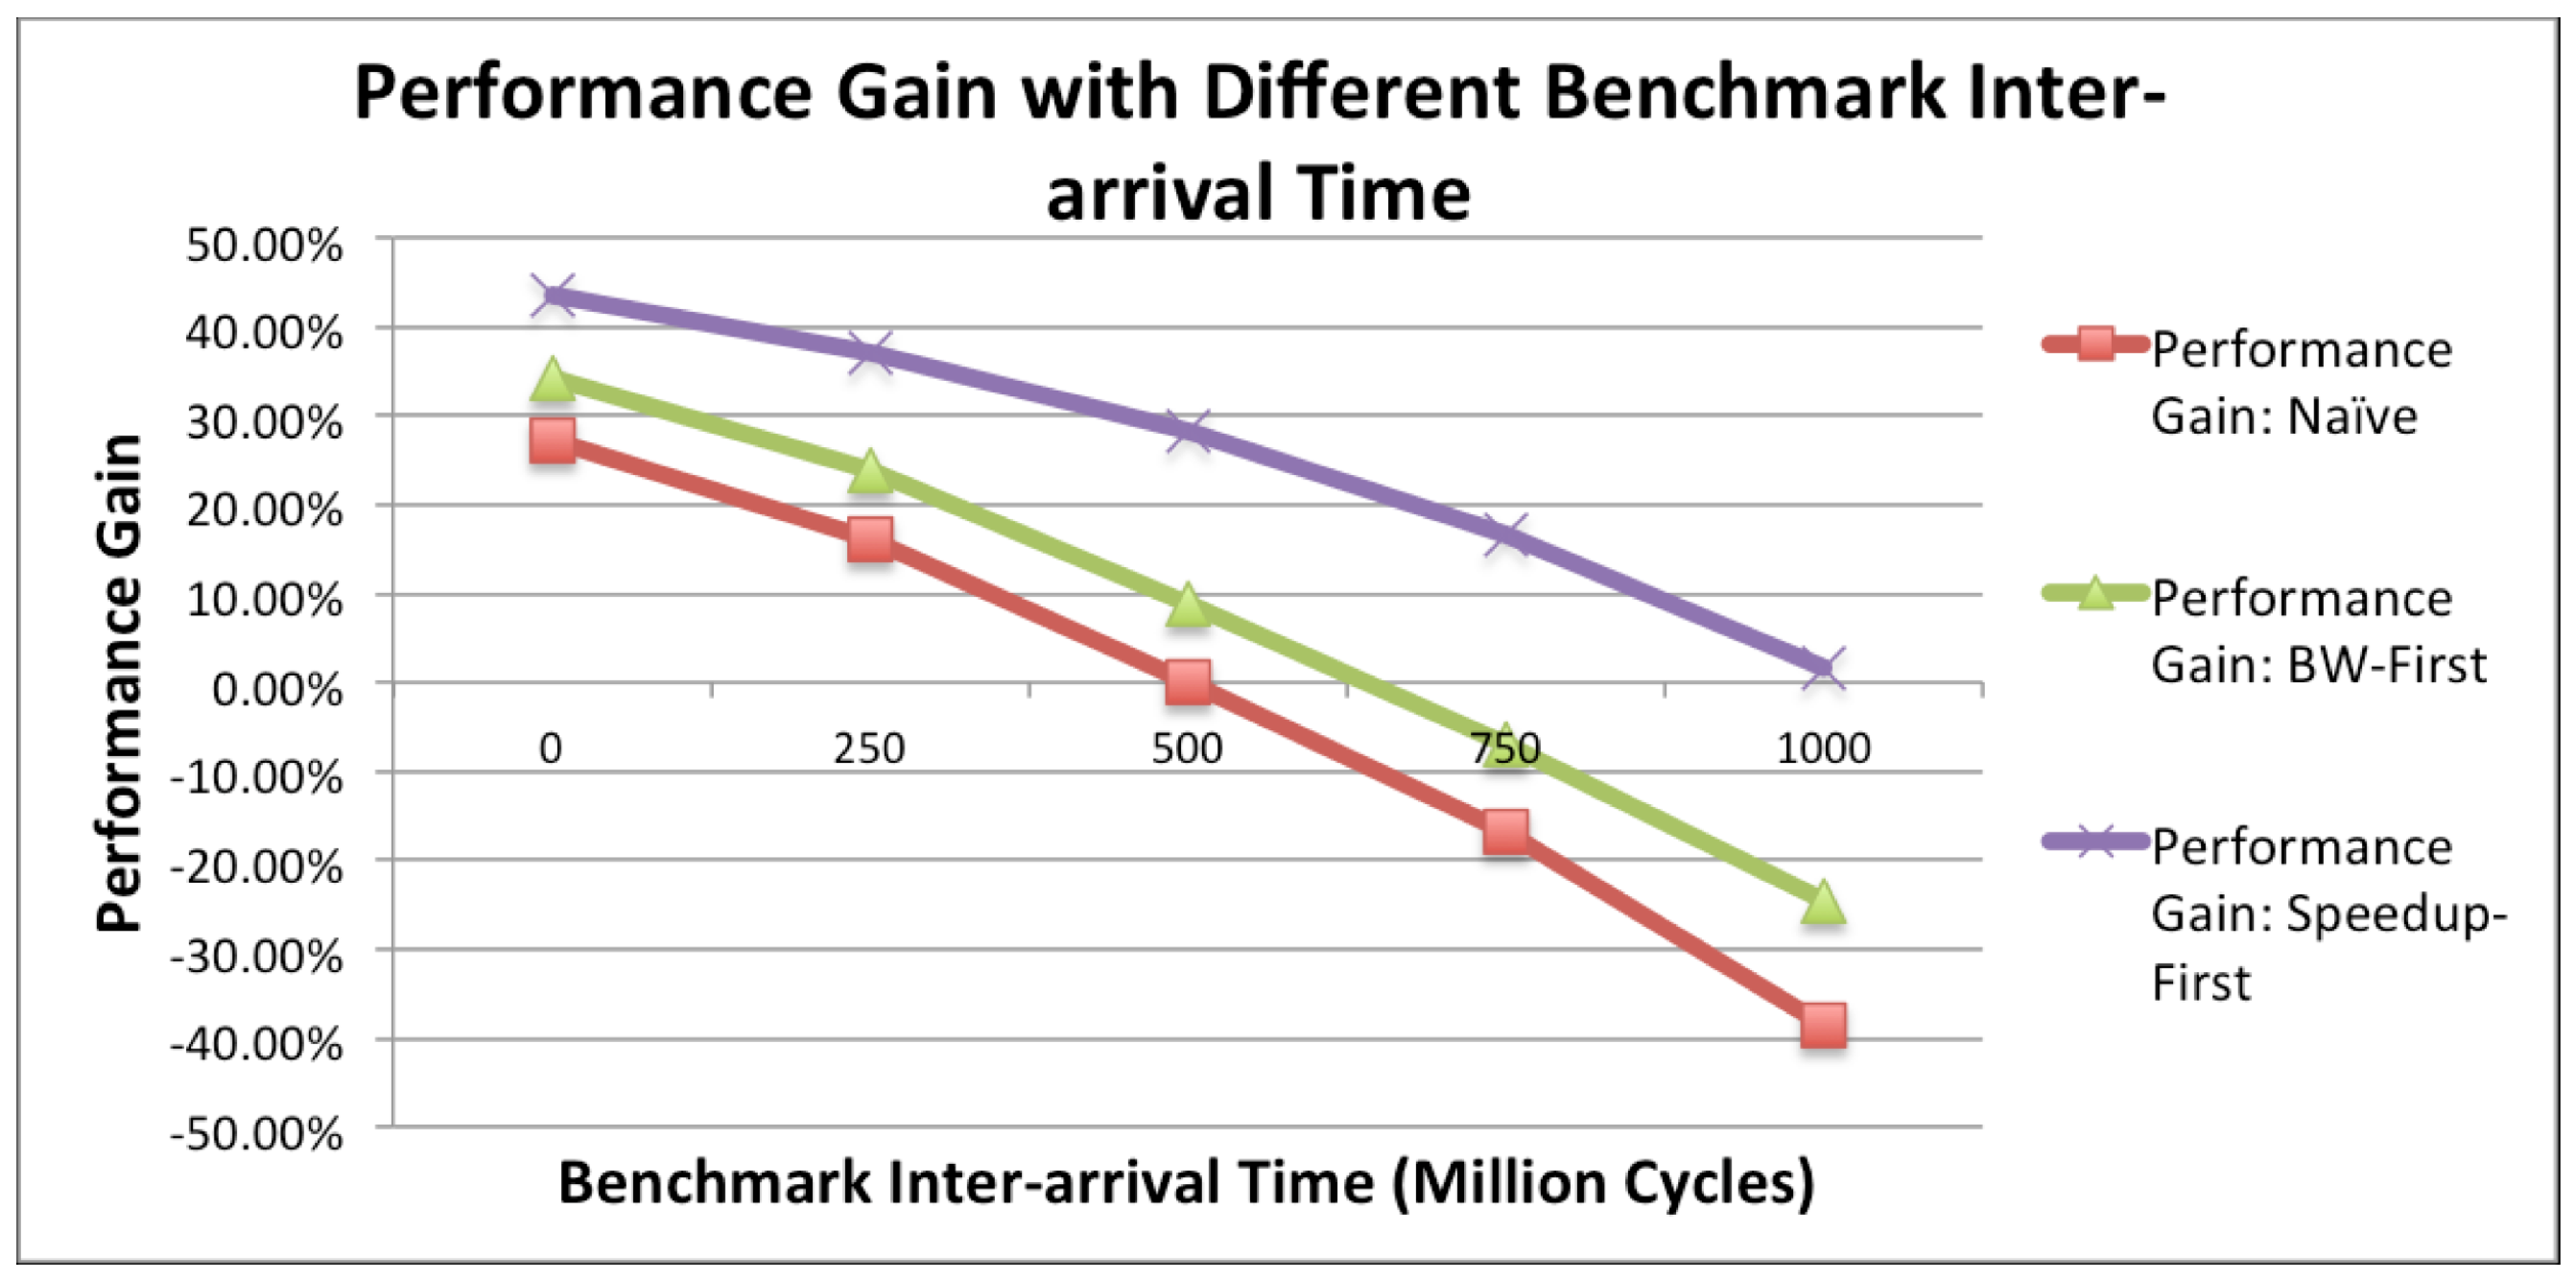
\includegraphics[width=4.5in]{Benchmark-Switching-Time}
    \caption{Performance Gain with Various Benchmark Inter-arrival Time}
    \label{fig_benchmark-switching}
\end{figure}

\subsubsection{Utilization of Reconfigurable Resources}

Figure \ref{fig_acc_timeline} shows a sample of the run-time
reconfiguration process on the {\em Transformer}. The x axis displays the
scheduling time window, while the y axis displays the number of acceleration
functions instantiated on the SoC. Figure \ref{fig_acc_timeline}
reveals the dynamics of the workload and how the {\em Transformer} adapts its
resources to the demanding functions. Figure \ref{fig_logic_timeline}
illustrates how the utilization of various resources within the
reconfigurable logic changes over time.

In addition, Figure \ref{fig_acc_timeline} validates the advantages of using run-time
configuration over fixed accelerators. We make the following observations regarding the maximum number of accelerators. 
The 3DES, SURF, Segmentation, and Smith-waterman functions all resulted in one
instantiation. The IDSI as well as the SLAM-J functions resulted in two instantiations. The SLAM-C as well as Jacobi functions resulted in 
three instantiations. To achieve the same performance relying on the fixed on-chip accelerators, 
the total amount of logic we would need includes: 17,848 SLICE elements, 14,511 FF elements, 13,192 LUT elements, and 255 BRAM elements. 
Specifically, we would need at least 3.8 times
more SLICE elements and 12.75 times more BRAM elements in order to perform comparably with the {\em Transformer}. 
The aforementioned findings serve as an example of the inefficient use of reconfigurable resources.


\begin{figure}[ht]
    \centering
    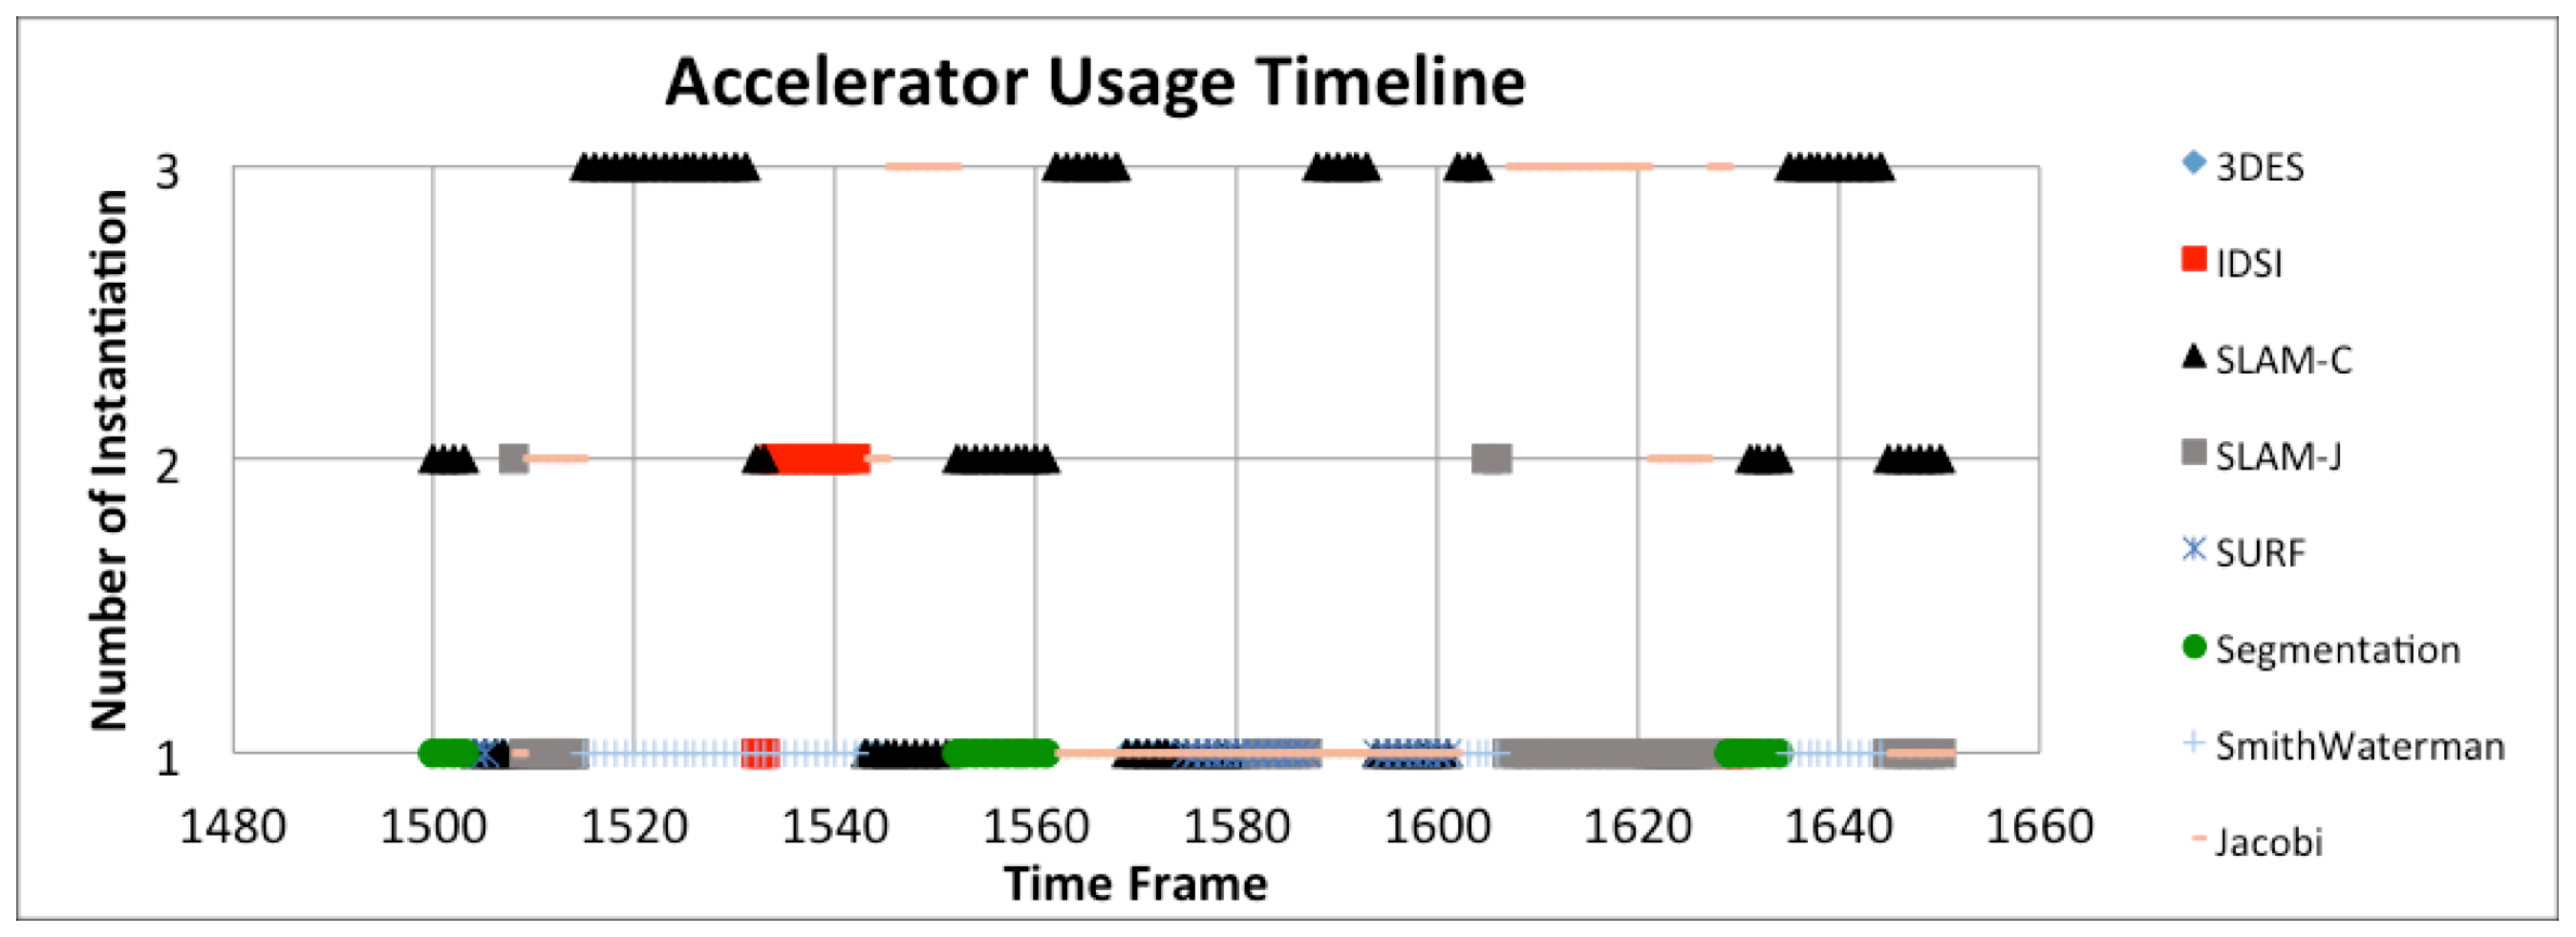
\includegraphics[width=6.0in]{Acc_timeline}
    \caption{Accelerator Usage Timeline}
    \label{fig_acc_timeline}
\end{figure}

\begin{figure}[ht]
    \centering
    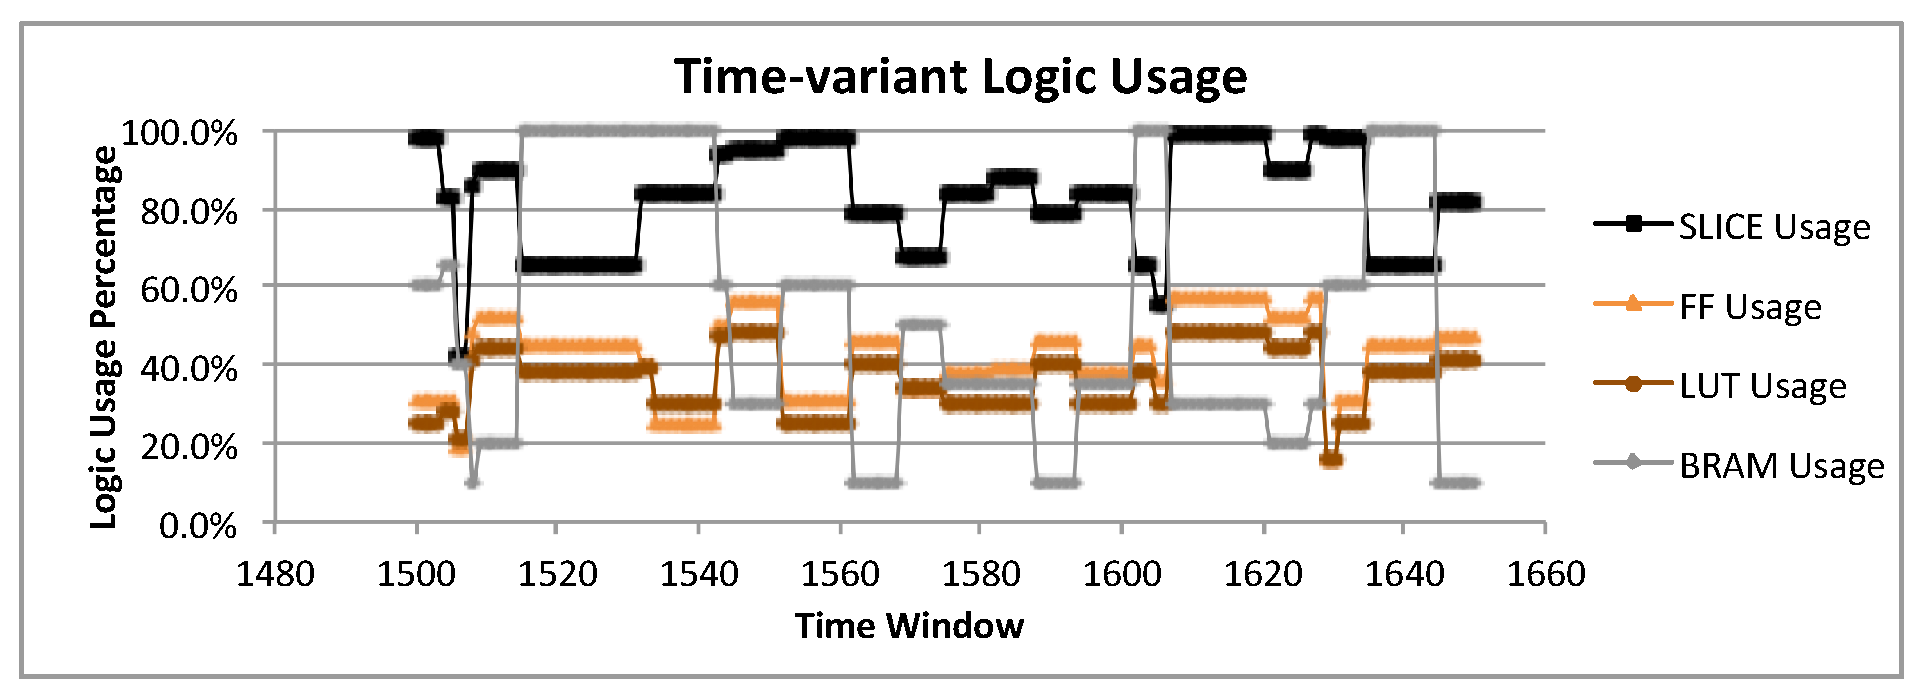
\includegraphics[width=6.0in]{Logic-Usage-Timeline}
    \caption{Total Logic Usage Timeline}
    \label{fig_logic_timeline}
\end{figure}


\section{Conclusion}
\label{sec_concl}

In this paper, we propose a heterogeneous architecture, the {\em
  Transformer}, consisting of on-chip, partially reconfigurable logic in order to
transparently accelerate dynamic, unpredictable workloads.
Middleware as well as the reconfiguration controller are introduced in order to trace the
run-time demands of the accelerator functions and invoke the acceleration
path. We derive two scheduling algorithms based on solving the Knapsack
problem in order to combine accelerators. We model the details of the
accelerators in a modified Multi2sim simulator and evaluate the
performance and the power efficiency of the {\em Transformer} with synthetic
workloads from a wide range of domains. The resulting performance and power
efficiency gains are shown to be significant. We study how the 
architectural parameters impact system performance and power. We
investigate the issues of chip area allocation with respect to the cores as well as the accelerators, and make notable observations 
regarding the optimal partitioning of the resources. 

In the near future, we plan to explore finer granularity
reconfigurable resources and accelerator-aware NoC to maximize the
performance of the {\em Transformer}. We also plan to compare the {\em Transformer}
with ASIC-based accelerators, which have significantly greater demands in terms of their VLSI
implementations. Furthermore, an FPGA-based prototype running real-world workloads obtained from cloud
servers is currently in development.

%In this paper, we propose a hybrid architecture with both general
%purpose cores and reconfigurable logic accelerators for power
%efficient computing, which is critical in both cloud computing and
%mobile devices. We also outline a control scheme to reconfigure the
%accelerator at run time in response to the dynamics of the
%workloads. We simulate such architecture with Simics based full system
%simulator by porting benchmarks and designing a device driver for
%accessing the accelerator from user-level threads. Our experimentation
%results show the effectiveness of the reconfigurable logic based
%accelerator and the run-time reconfiguration. This 
%preliminary study encourages us to investigate the performance of the proposed hybrid
%architecture in virtualization environments. 
%%We also plan to optimize the run-time
%%reconfiguration schemes for higher speedup, for example, considering
%%not only the demand of a function, but also the speedup of
%%the accelerated functions.


\section{Acknowledgment}
\label{sec_ack}

This work is supported in part by Intel Embedded University Program.


%-------------------------------------------------------------------------
\bibliographystyle{elsarticle-num}

\bibliography{reference}

\end{document}

